\chapter{DeepGeo: Deep Geometric Mapping for Shape Parameterization}
\label{ch5}

This chapter is based on the conference paper \cite{aa.Wei2024b} and the journal paper \cite{aa.Wei2025}.

\textbf{Zhen Wei}, Aobo Yang, Jichao Li, Michaël Bauerheim, Rhea P. Liem, and Pascal Fua, "DeepGeo: Deep Geometric Mapping for Automated and Effective Parameterization in Aerodynamic Shape Optimization,” in AIAA Aviation Forum, 2024. https://doi.org/10.2514/6.2024-3839. 

\textbf{Zhen Wei}, Aobo Yang, Jichao Li, Michaël Bauerheim, Rhea P. Liem, and Pascal Fua, “Automated Parameterization for Aerodynamic Shape Optimization via Deep Geometric Learning,” AIAA Journal, 2025. https://doi.org/10.2514/1.J065203.

\section{Nomenclature}

{\renewcommand\arraystretch{1.0}
\noindent\begin{longtable*}{@{}l @{\quad=\quad} p{0.8\textwidth}@{}}
$\alpha$            &  the angle of attack \\
$C_D,\;C_L,\;C_{M}$&  drag, lift and pitching moment coefficients\\
$\mathfrak{C}$       &  the subset of DeepGeo's input coordinate space that defines the CFD computational domain \\
$f_\Theta,\;\Theta$ &  the Deep Geometric Mapping model and its weights \\
$g$                 &  the adjoint solver \\
$L$                 &  the loss function and the soft constraint \\
$M, V, E$           &  the CFD mesh and its vertices, edges \\
$O$                 &  the optimization objective \\
$P$                 &  FFD control points \\
$S$                 &  the initial object geometry for optimization \\
$t,A,Vol$             &  the geometry's thickness, area and volume \\
$V^S,\;V^F,\;V^V$   &  CFD mesh vertices on the objects surface, fixed patches and in the volumetric grids
\end{longtable*}}

\section{Introduction}

Aerodynamic Shape Optimization (ASO) is a process aimed at refining an object’s shape design to enhance its aerodynamic performance, achieving objectives such as reducing fuel consumption, increasing operating efficiency or improving maneuverability, under specified design constraints. ASO holds significant importance across various fields where it facilitates designs for applications like aerospace, automotive, and marine engineering. As shown in Fig.~\ref{ch5:fig:aso_pipeline}(a), ASO typically involves iterative cycles of computational fluid dynamics (CFD) simulations, visualization and expert analysis, shape modeling and modification, and mesh deformation or remeshing. Traditional ASO can be both slow and costly, with shape parameterization and its associated geometric processing being especially labor-intensive.

Shape parameterization is central to ASO. It provides the mathematical framework through which object geometries are represented and manipulated. Its influence on ASO performance is both profound and multifaceted. The choice of parameterization approach defines the optimization boundaries, determining the maximum geometric complexity that can be handled, the allowable range of shape modifications, and the achievable level of surface smoothness. Then a key challenge lies in balancing the dimensionality of the parameter space with optimization effectiveness: a high-dimensional parameter space enables detailed geometric modeling but may hinder convergence, while a lower-dimensional space facilitates faster optimization but can restrict the search within the design space. Furthermore, the parameterization method directly impacts ASO’s implementation costs due to the level of human intervention required: from initial surface modeling and design variable configuration to the management of CFD mesh deformation. Consequently, selecting an effective parameterization approach is critical for achieving cost-effective and efficient ASO.

Given its critical importance, shape parameterization has been the focus of extensive research. Traditional approaches include Hicks-Henne bump functions~\cite{aa.Hicks1978}, non-uniform rational B-spline (NURBS) curves, and class-shape function transformation (CST)\cite{aa.Kulfan2008} for two-dimensional applications, while free-form deformation (FFD)~\cite{aa.Sederberg1986, aa.Lamousin1994, aa.Kenway2010} is preferred for three-dimensional problems. Despite their success, these traditional methods face notable challenges. The performance and computational efficiency of ASO are highly sensitive to how the parameterization is implemented, including the choice of algorithm and hyperparameters~\cite{aa.Masters2017,aa.Vuruskan2019,aa.Song2004}, with no formal methodology to identify optimal configurations. This leads practitioners to rely on trial-and-error approaches, empirical knowledge, or adaptation of methods from similar cases, followed by extensive manual tuning. This reliance on manual processes makes traditional methods impractical for rapid prototyping and iterative design, where efficiency and adaptability are crucial. Moreover, designers must balance trade-offs between deformation freedom, optimization effectiveness, and global surface smoothness. While high-dimensional design variables provide greater design flexibility, they complicate optimization and increase the risk of poor convergence. Ensuring global surface smoothness is also challenging with large deformation freedom, where even minor surface inconsistencies can cause glitches in simulation, disrupting the optimization process.
Furthermore, traditional parameterizations solely focus on the surface geometry, necessitating separate processing of volumetric CFD meshes through deformation or re-meshing, which adds substantial implementation complexity. While AI-based parameterization models have emerged as alternatives~\cite{aa.Bamford2024,aa.Swannet2024,aa.Secchi2024}, their data-driven nature requires a large-scale training dataset and introduces new challenges on data engineering, particularly in aerospace applications where training data is scarce and computationally expensive to generate. The geometric priors learned by these models are inherently limited by the dataset available, making any newly generated shape an interpolation of existing data rather than a truly novel design. Consequently, AI-based models lack the innovation potential of free-form parameterization methods, which offer greater design space exploration.

To address these limitations, we aim at building an AI-assisted ASO pipeline and introduce the Deep Geometric Mapping (DeepGeo) model, a novel neural network-based approach that unifies shape representation and mesh deformation within a single framework, as shown in Fig.~\ref{ch5:fig:aso_pipeline}(b). DeepGeo uses a Multi-Layer Perceptron (MLP) to parameterize both the surface geometry and the surrounding CFD computational volumetric mesh, the latter being necessary for aerodynamic performance evaluation through CFD simulations. 
As illustrated in Fig.\ref{ch5:fig:pipeline}(a), DeepGeo's initialization phase involves training the MLP to deform the surface vertices from a template shape to align with the target geometry, the starting configuration for optimization.
The surrounding volumetric mesh is simultaneously deformed to ensure consistency with the surface geometry. By accurately reconstructing the target geometry, this initialization process encodes the geometric information within the network weights. 
Shape optimization is then performed by applying an adjoint-based method~\cite{aa.Jameson1995} to minimize aerodynamic objective functions and enforce geometric constraints with respect to these weights, as shown in Fig.\ref{ch5:fig:pipeline}(b). 
The updated weights enable DeepGeo to output a CFD mesh that defines a new geometry, thus manipulating the shape design iteratively. The optimization process continues until convergence is reached.
This formulation establishes the network weights as the parameterization for both the surface shape and the volumetric mesh, enabling automated regeneration of the necessary CFD mesh as the geometry evolves with every optimization iteration. By unifying shape parameterization and mesh deformation within a single framework, DeepGeo significantly reduces traditional ASO implementation complexities and streamlines the optimization pipeline, by removing the need for a separate CFD mesh deformation or remeshing module and the associated time-consuming manual hyperparameter tuning. This simplification accelerates the ASO process.

% !TEX root = ../main.tex
% !TEX spellcheck = en-US

\begin{figure}[tbh]
    \begin{center}
        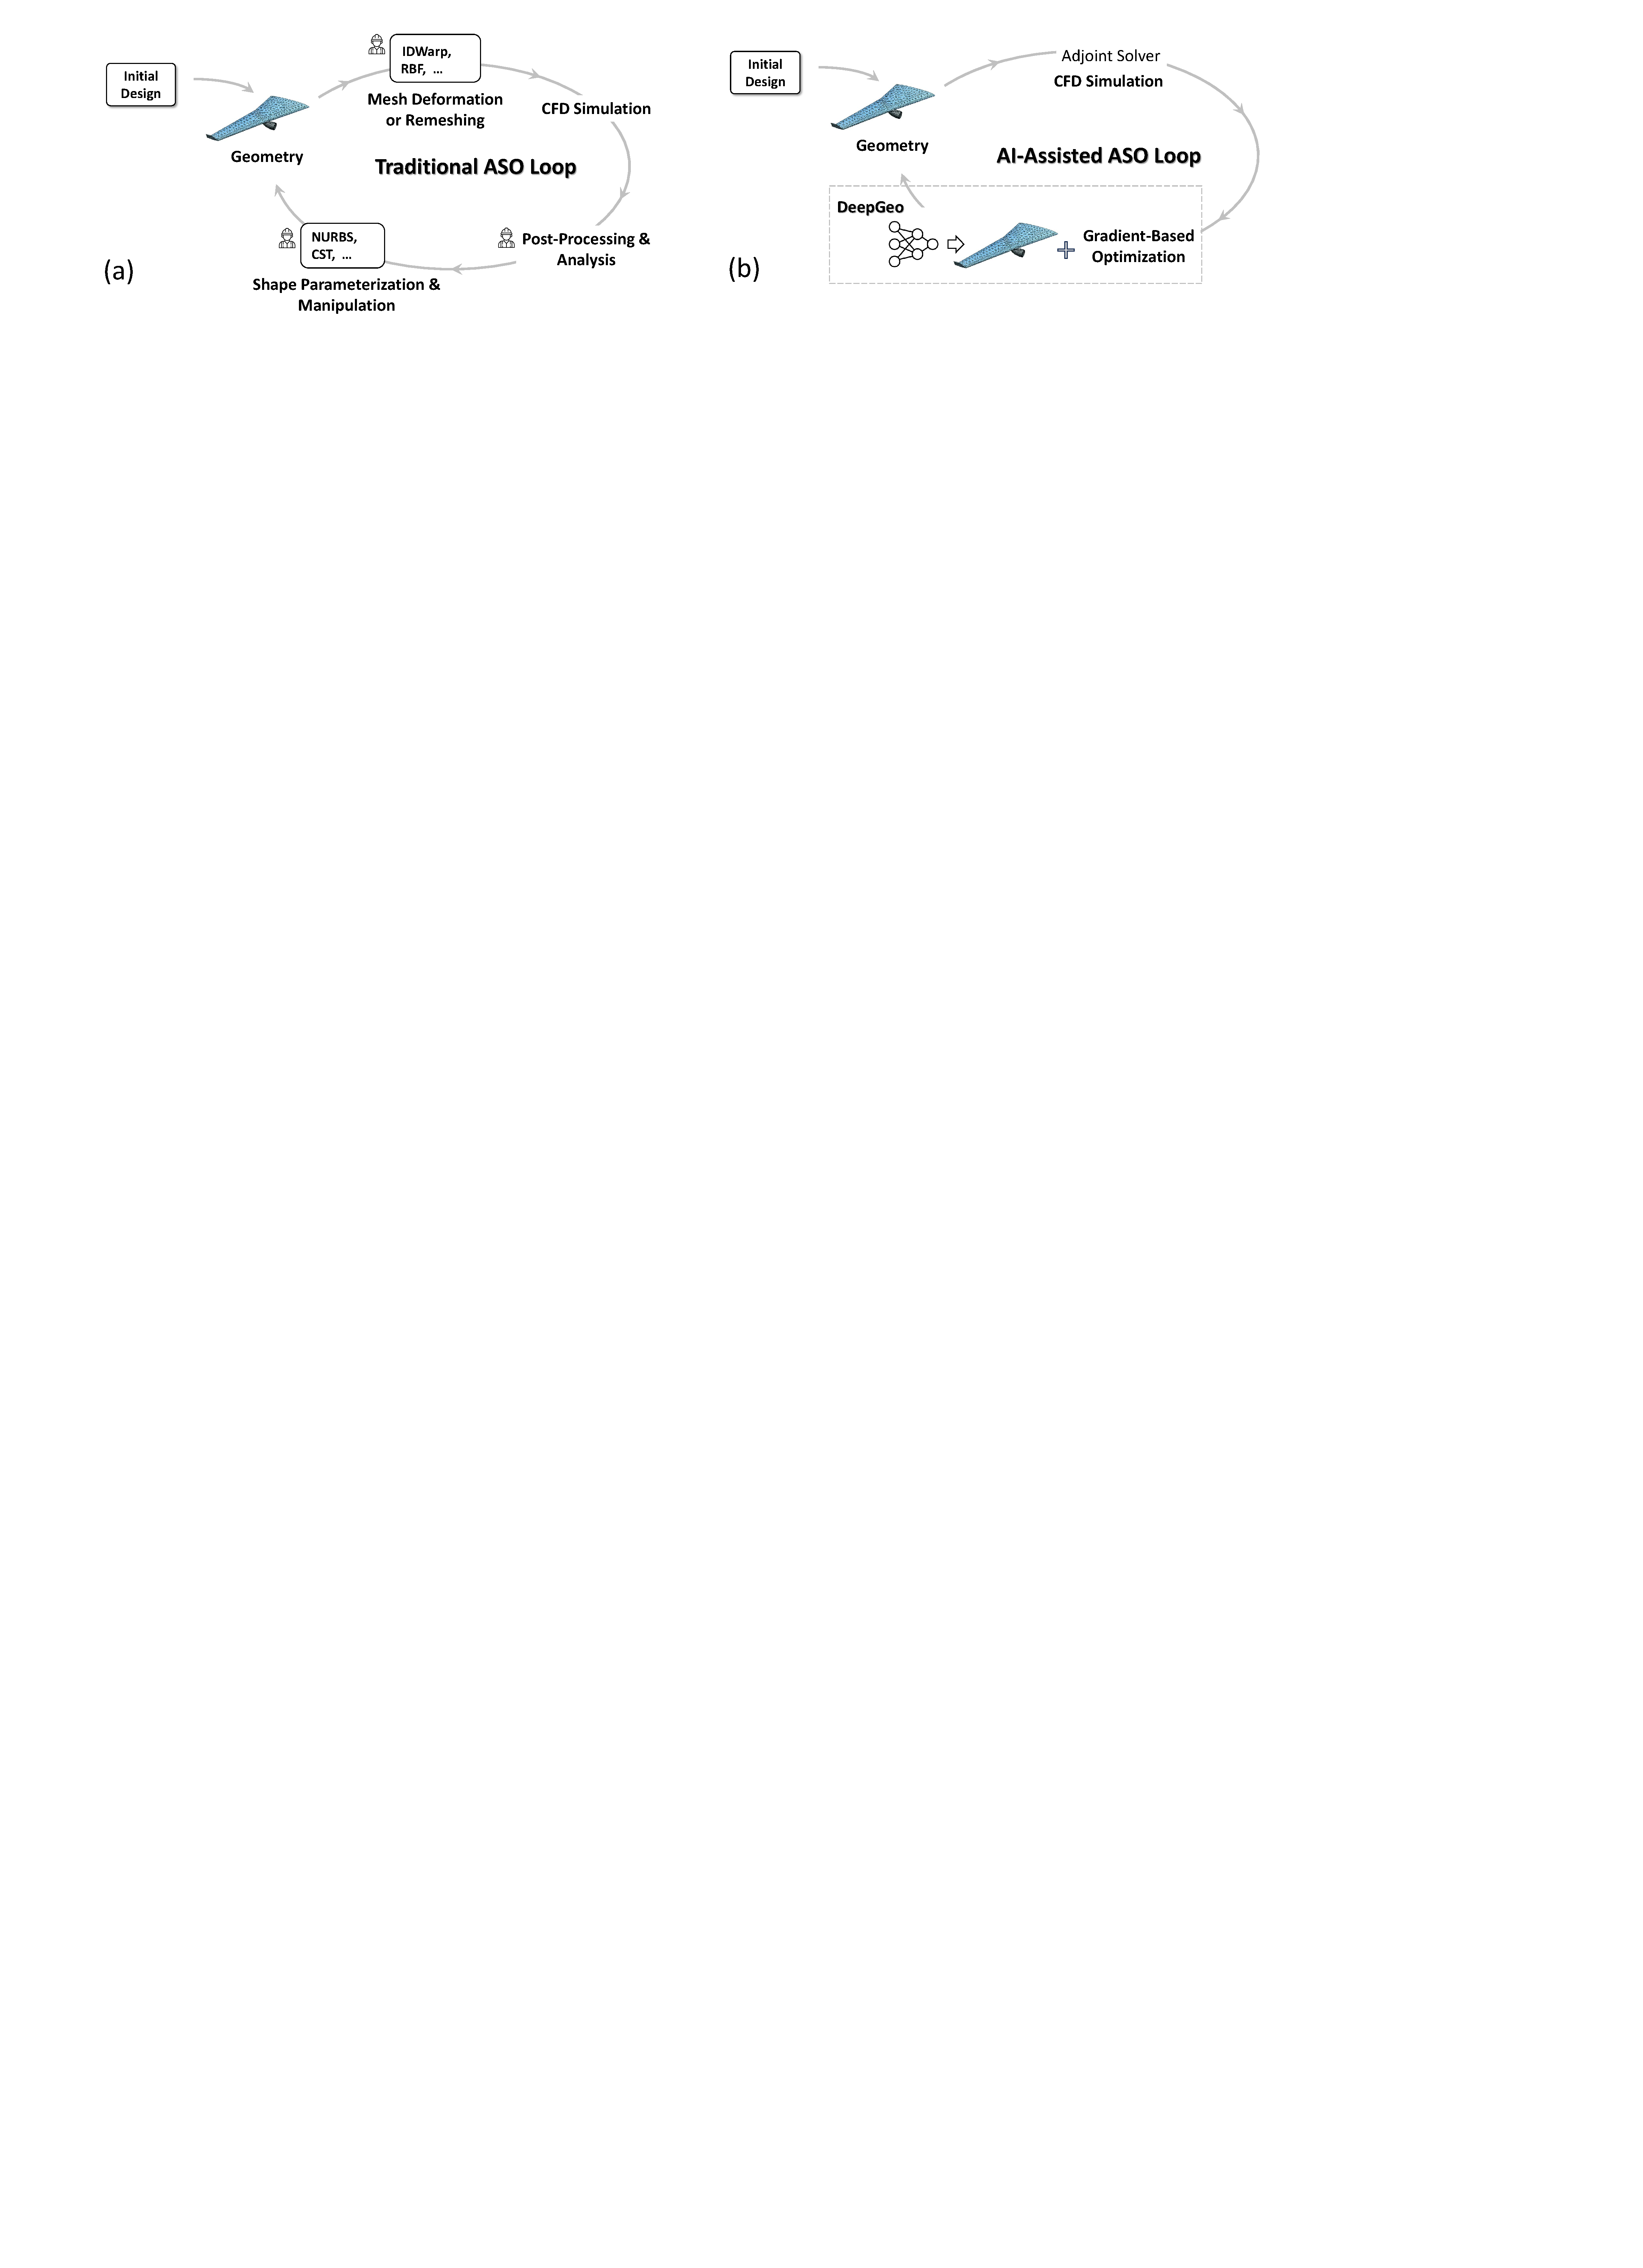
\includegraphics[width=1\linewidth]{chapter5/fig/aso_pipeline.pdf}
    \end{center}
    \vspace{-3mm}
    \caption{
        \small The pipelines of (a) traditional ASO and (b) ASO that employs DeepGeo.
    }
    \label{ch5:fig:aso_pipeline}
\end{figure}
% !TEX root = ../main.tex
% !TEX spellcheck = en-US

\begin{figure}[tbh]
    \begin{center}
        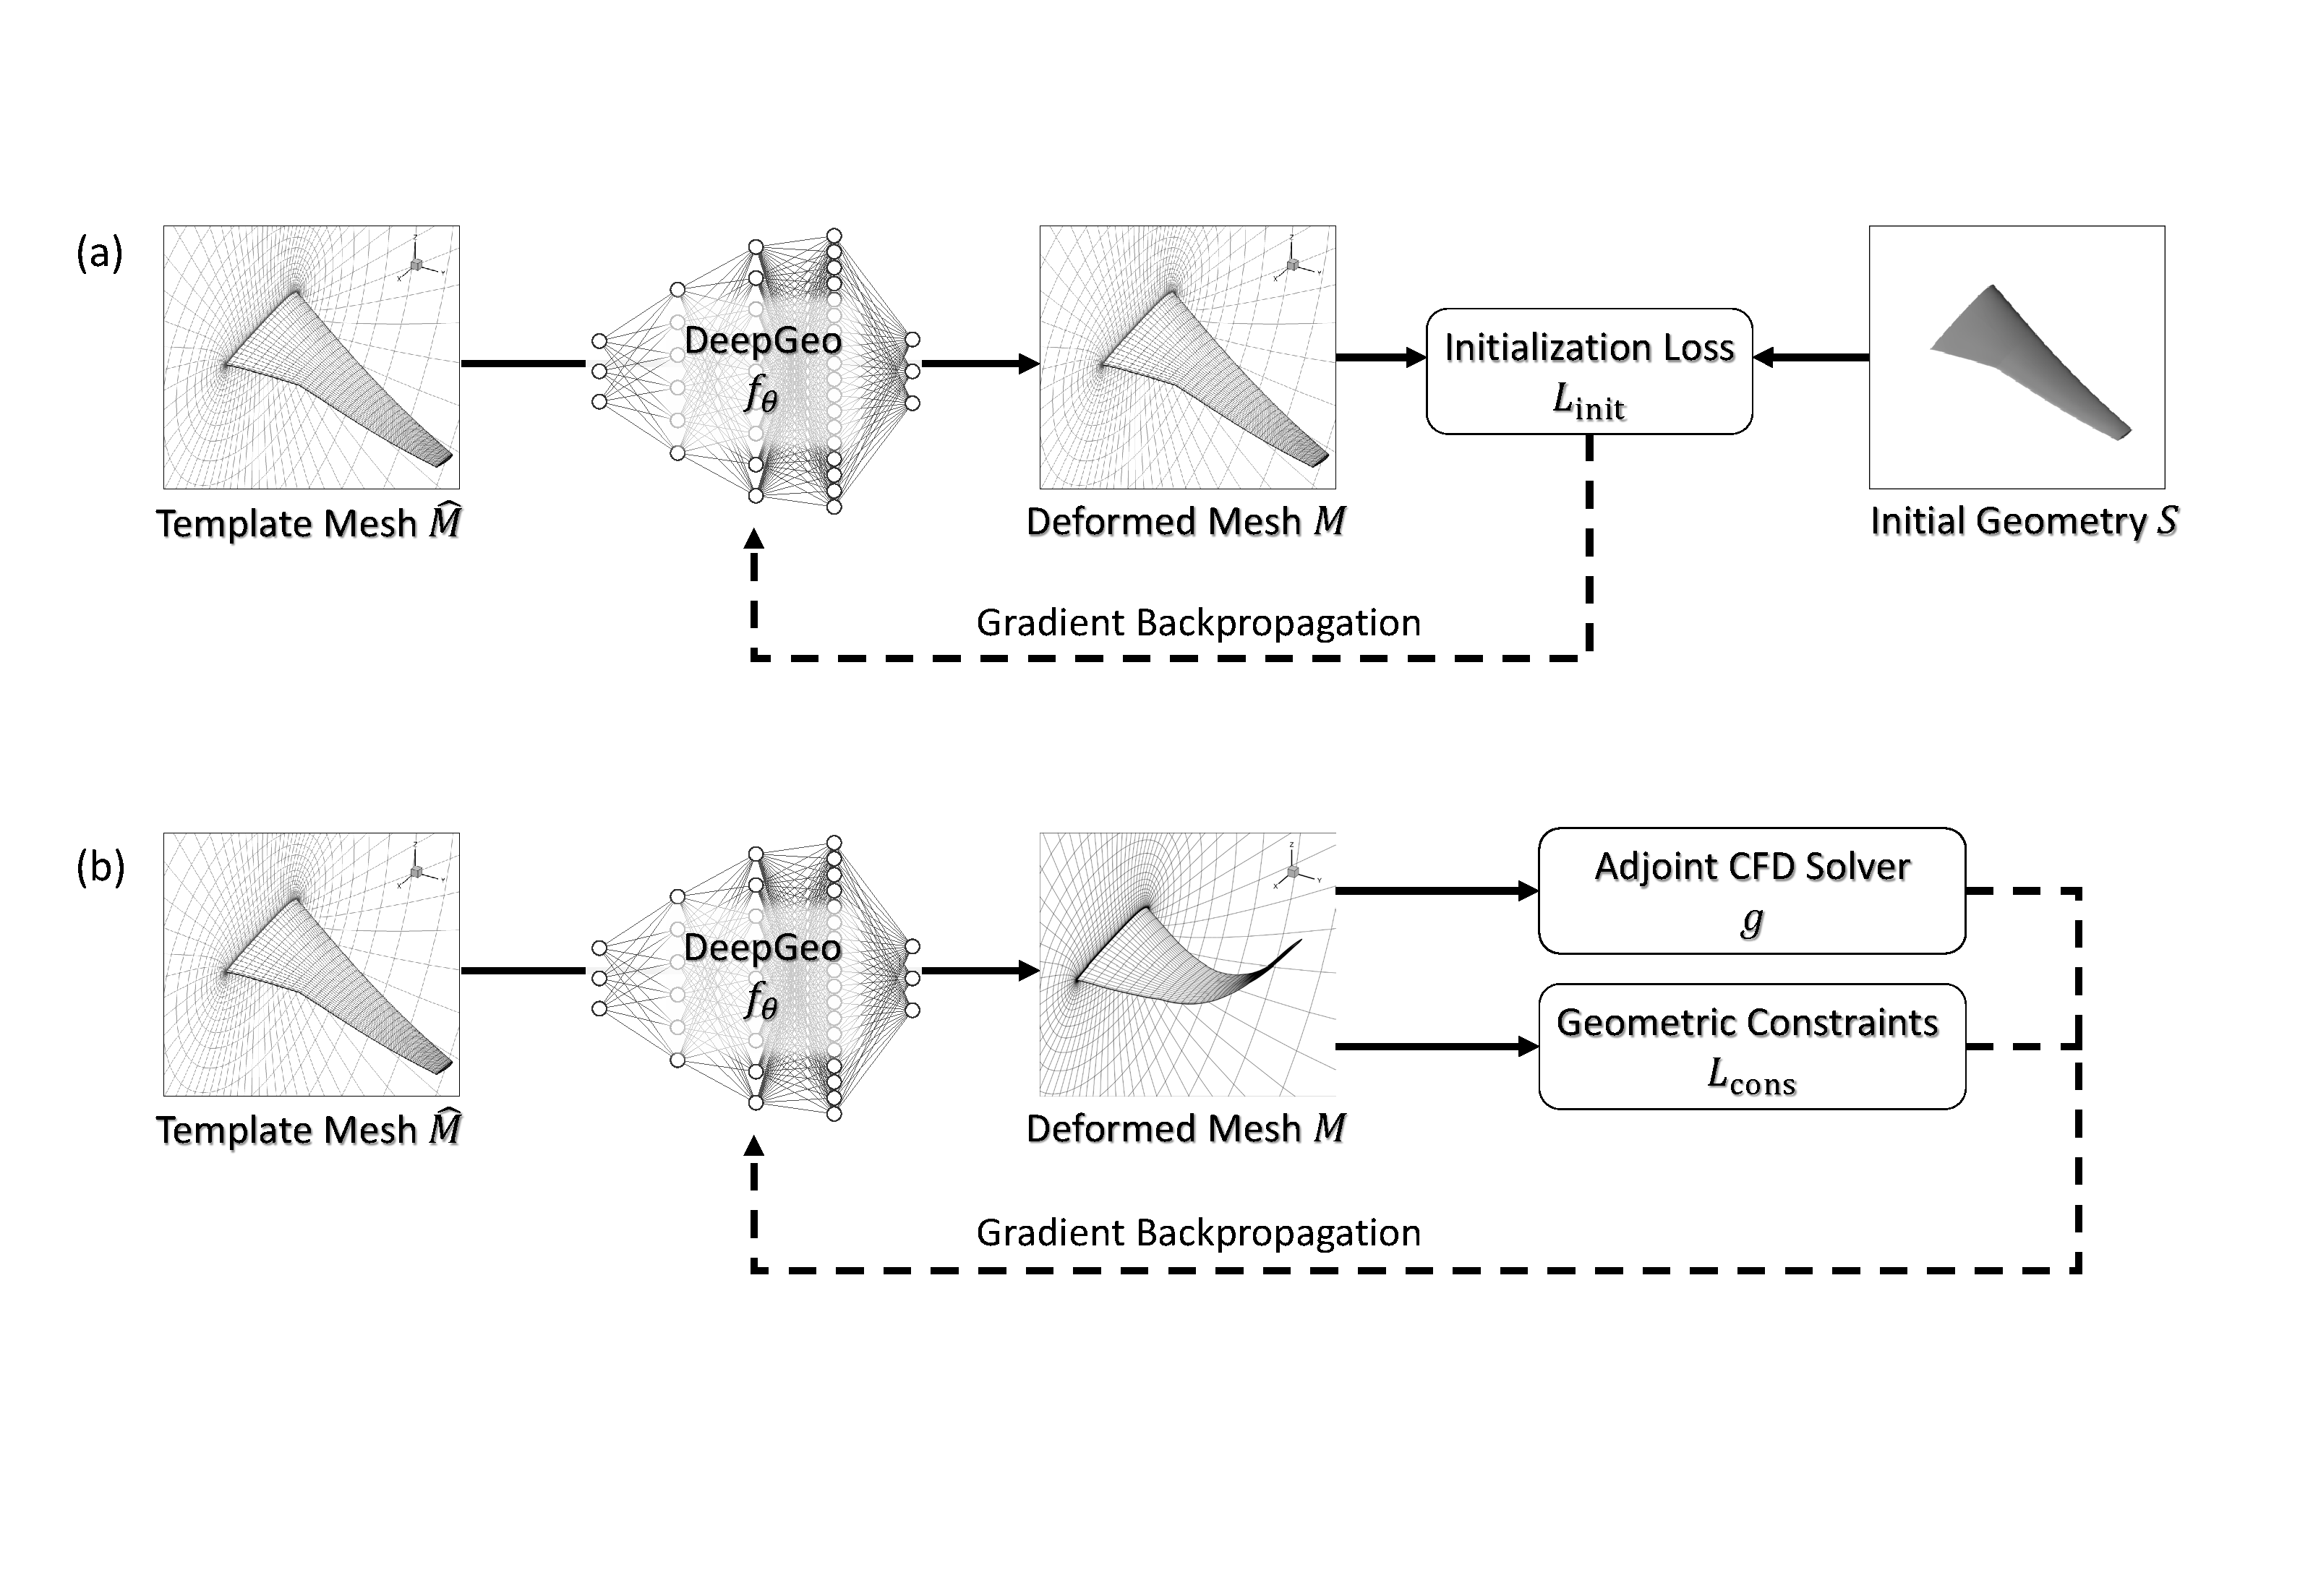
\includegraphics[width=1\linewidth]{chapter5/fig/pipeline.pdf}
    \end{center}
    \vspace{-3mm}
    \caption{
        \small The pipeline that employs DeepGeo in ASO, including (a) the initialization and (b) shape optimization stages.
    }
    \label{ch5:fig:pipeline}
\end{figure}
\begin{figure}[!htb]
    \begin{center}
        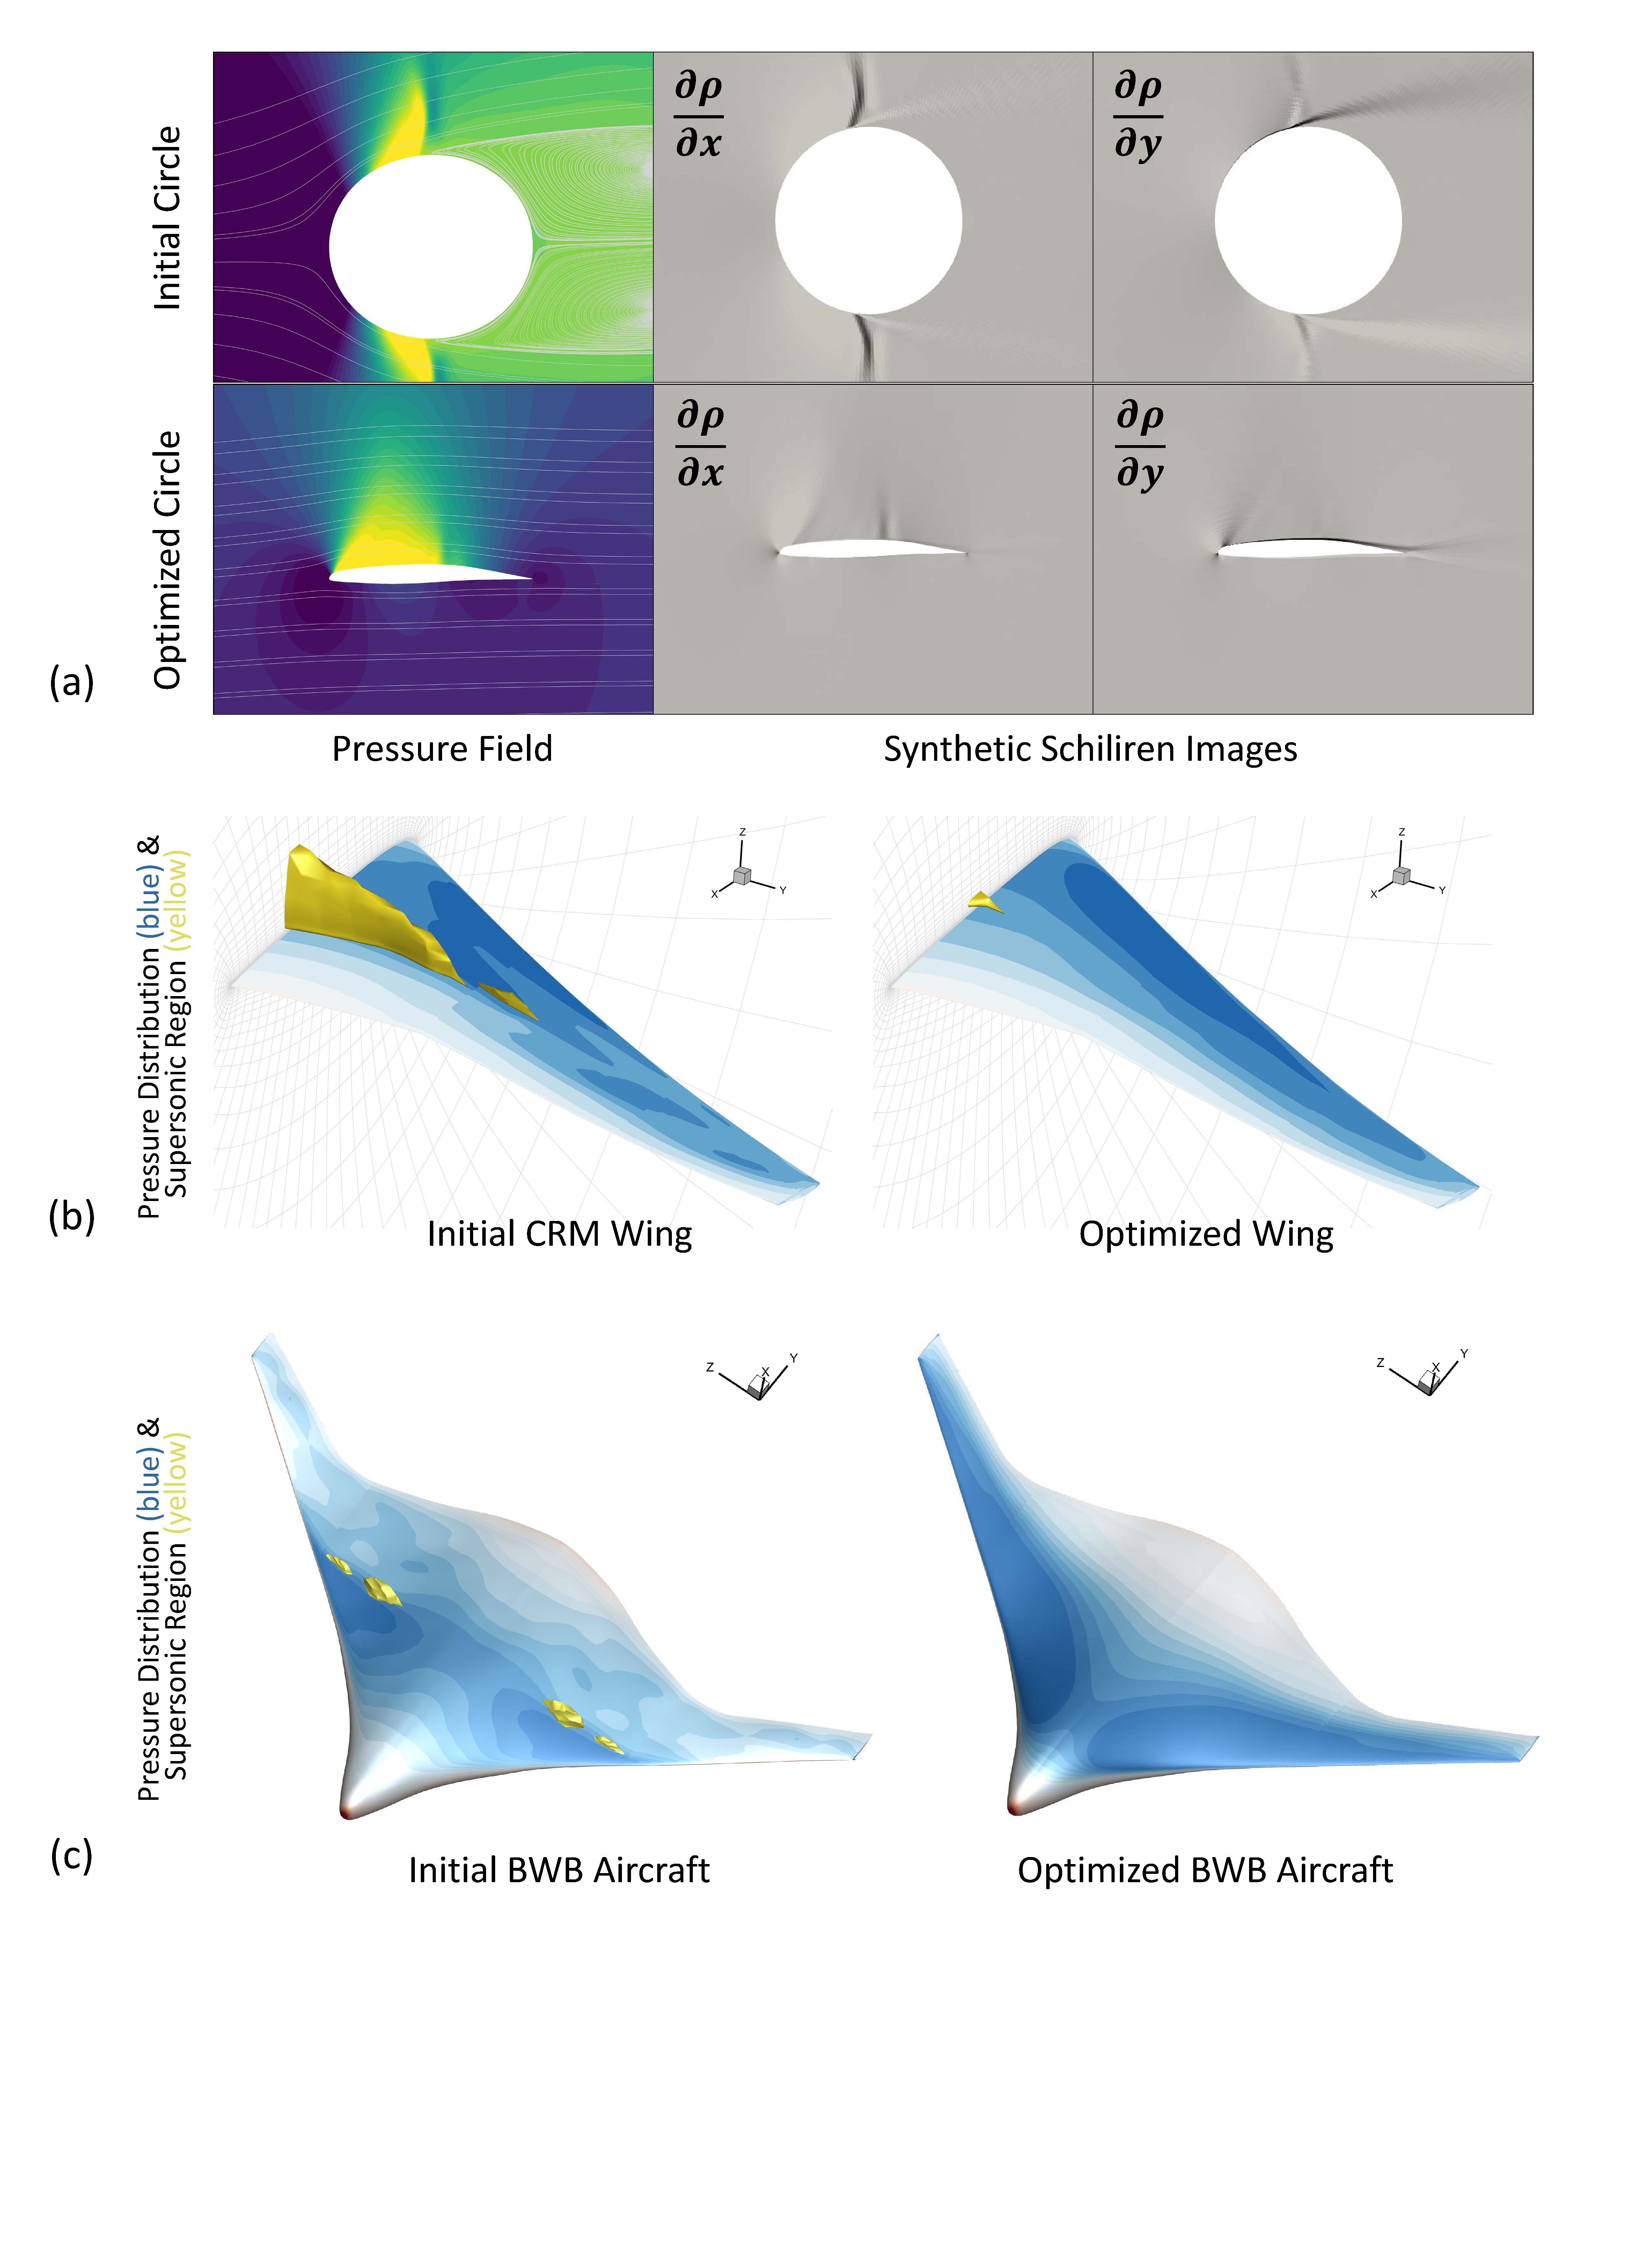
\includegraphics[width=0.9\linewidth]{chapter5/fig/teaser.pdf}
    \end{center}
    \vspace{-3mm}
    \caption{
        \small The three ASO case studies implemented by DeepGeo, including optimization from (a) 2D circle, (b) CRM wing and (c) BWB aircraft.
    }
    \label{ch5:fig:teaser}
\end{figure}

DeepGeo leverages the expressive capacity of MLPs, which comes from their ability to represent complex nonlinear mappings as layered compositions of simple functions. Thus, DeepGeo can capture rich geometric transformations and handle large deformations, while maintaining global surface smoothness. This expressiveness is key to achieving smooth, continuous transformations across complex geometries, a critical ability in high-fidelity shape optimization. DeepGeo's MLP backbone makes it possible to explore high-dimensional design spaces using a gradient-based approach by mitigating the curse of dimensionality or issues with over-parameterization~\cite{ai.Barron1993,ai.Poggio2017}. DeepGeo directly addresses the dimensionality challenges that limit traditional optimization methods, such as CMAES~\cite{ai.Hansen2016}, which become impractical beyond approximately 100 design parameters. 
Furthermore, DeepGeo’s initialization requires only a target shape and a single template mesh to set its initial weights, in contrast to data-driven approaches that rely on extensive training datasets. This minimal data requirement significantly reduces implementation complexity, decreasing dependency on large datasets and making DeepGeo especially suitable for practical aerospace applications where geometric data is often scarce.

In earlier work~\cite{aa.Wei2023b}, we introduced the Direct Mapping Model, an initial version of DeepGeo developed to handle 2D airfoil optimization. In this paper, we extend the model to address more complex optimization tasks and 3D shapes, including 2D circle optimization, 3D wing optimization, and the optimization of a 3D Blended-Wing-Body aircraft. DeepGeo achieves optimization results comparable with the state-of-the-arts, without any case-specific adaptation and requiring training dataset, as shown in Fig.~\ref{ch5:fig:teaser}.
\section{Related Work}
\label{ch5:sec:related_work}

DeepGeo spans across multiple research domains, including the shape parameterization algorithms in computer graphics and aerodynamic shape optimization studies, as well as self-prior models in deep learning research. Each part will be briefly reviewed, and the DeepGeo's technical prominence will be discussed afterward.

\subsection{Shape Parameterization in Aerodynamic Shape Optimization}
Shape parameterization in ASO refers to the mapping of explicit design variables to the object's surface mesh, a fundamental module for effectively solving ASO problems. \citet{aa.Jameson1988} introduced a direct conformal mapping from a circle to optimize airfoils, which provided the maximal design freedom in design space but lacked sufficient smoothness for CFD solvers~\cite{aa.Braibant1984}. Therefore, shape parameterization is necessary to reduce the design space dimensionality and introduce smoothness control. It can be broadly categorized as non-data-driven and data-driven approaches. 

\subsubsection{Non-Data-Driven Approaches}

Non-data-driven algorithms include both constructive and deformative methods~\cite{aa.Masters2017}. Constructive methods, such as polynomial/spline based methods~\cite{aa.Kulfan2008,aa.Braibant1984,aa.Farin1995} and partial differential equation methods~\cite{aa.Bloor1995,aa.Smith1995}, represent the airfoil surface based on specified parameters. Deformative methods deform an existing shape, including analytical methods~\cite{aa.Hicks1978,aa.Pickett1973,aa.Hager1992} and the free-form deformation (FFD)~\cite{aa.Sederberg1986, aa.Lamousin1994, aa.Kenway2010}. Early analytical approaches, like the Hicks-Henne bump function~\cite{aa.Hicks1978} and others~\cite{aa.Pickett1973,aa.Hager1992}, optimized the shape through linear combinations of basis functions. B-splines~\cite{aa.Braibant1984} and its variants, like the Bezier curve and nonuniform rational B-spline (NURBS)~\cite{aa.Farin1995}, use control points and piece-wise polynomials to define the geometry. Polynomial-based methods like parameterised sections (PARSEC)~\cite{aa.Sobieczky1999} and CST~\cite{aa.Kulfan2008} approximate surfaces with weighted sums of polynomials with different orders. While effective, these methods are suited for 2D curves. The FFD, originating from soft object animation in computer graphics~\cite{aa.Sederberg1986,ai.Barr1984,aa.Lamousin1994}, enables smooth continuous volume transformations based on control point movements. It is widely used in optimizing 3D objects like the CRM wing~\cite{aa.Lyu2015,aa.Wu2022} and the overall aircraft~\cite{aa.Secco2021}.

When applied to infinite-dimensional problems with finite-dimensional design variables, non-data-driven methods require compromising between the dimensionality for effective parameterization and the optimization complexity~\cite{aa.Ceze2009}. Additionally, the lack of self-adaptation leads to heavy reliance on expert knowledge and manual tuning for hyperparamters. As such, different settings can significantly impact optimization results. To address these limitations, DeepGeo bases on the neural network which provides universal approximation ability~\cite{ai.Barron1993} and mitigates the curse of dimensionality~\cite{ai.Barron1993,ai.Poggio2017}.

\subsubsection{Data-Driven Approaches}

Data-driven methods aim to reduce the dimension of design variables using existing geometry datasets, facilitating effective optimization for challenging problems or extracting patterns to reduce human intervention~\cite{aa.Li2022b}. Linear dimension reduction methods use proper orthogonal decomposition (POD) to derive a set of orthogonal modes. This can be done by Gram-Schmitt orthogonalization~\cite{aa.Robinson2001} or applying a singular value decomposition (SVD) to find orthogonal shape modes from a dataset~\cite{aa.Poole2015,aa.Li2019,aa.Kedward2020}. However, reconstructing the geometry from a latent vector remains challenging and requires dedicated manual designs for specific tasks. The active subspace model (ASM)~\cite{aa.Constantine2014,aa.Li2019b,aa.Lukaczyk2014,aa.Namura2017,aa.Grey2018} and active subspace identification (ASI)~\cite{aa.Bauerheim2016} reduce the dimensionality by analyzing the gradient from surrogate models for surrogate-based optimization or uncertainty quantification. Random sampling methods were used to estimate the real active subspace. However, generating valid samples requires handcrafted rules, and the approximation error is upper bounded by the Poincar\'{e} constant, which increases with dimensionality given a limited number of samples~\cite{ai.Payne1960,ai.Beyer1999}. Among the non-linear approaches, \citet{aa.Viswanath2011} proposed the generative topographic mapping (GTM) that projects a 30-dimensional design variable into a 2D latent vector. GTM's Bayesian generative model makes it challenging to integrate its latent representation into a gradient-based pipeline. More recently, generative models has been used for novel geometry generation \cite{aa.Achour2020,aa.Chen2020,aa.Li2020,aa.Li2021,aa.Wei2024,aa.Yang2024} to improve the quality of dimension reduction~\cite{aa.Li2020,aa.Li2021} or serve as a parameterization model directly~\cite{aa.Achour2020,aa.Chen2020}.

Data-driven methods typically demand large datasets for training~\cite{aa.Li2022b,aa.Wei2023,aa.Li2019}. DeepGeo stands out for its high data-efficiency as it requires only a single initial geometry for training, without requiring any additional user input comparing to the traditional ASO pipeline. This characteristic makes it a feasible solution for complex 3D geometries with limited data availability.

\subsection{Shape Parameterization in Computer Graphics}
Shape parameterization in computer graphics aims to create bijective mappings between two surfaces or volumes, with one domain represented as a mesh~\cite{ai.Sheffer2006}. This long-standing and active research field has diverse applications, like in mesh morphing, smoothing, remeshing, and so on. Creating one-to-one mappings between coordinate spaces inevitably introduces distortions that need to be minimized to retain desired mesh properties. Research has focused on surface mesh parameterization using cost functions that include distortion metrics, leading to the development of angle-preserving/conformal mappings, area-preserving/authalic mappings~\cite{ai.Floater2005,ai.Sheffer2006}, as-rigid-as-possible transformation~\cite{ai.Sumner2004,ai.Sorkine2007}, least squares conformal mapping~\cite{ai.Levy2002} and Dirichlet energy minimization methods~\cite{ai.Schreiner2004,ai.Smith2015,ai.Terzopoulos1987b}. DeepGeo extends the previous research focus to surface and triangulated meshes so that it works with complicated volumetric and unstructured CFD meshes. DeepGeo aligns more closely with the concept of a computer graphics parameterization model, as it establishes a mapping between volumetric CFD meshes instead of generating a design variable vector.

While early ASO shape parameterization methods were inspired by computer graphics, they are not directly applicable to volumetric CFD meshes.  DeepGeo’s key contribution lies in its regularization loss, which efficiently implements constrained volumetric mesh parameterization. Specifically, DeepGeo's regularization loss is derived from the continuous manifold learning theory, eliminating the need for mesh topology and allowing for flexible and highly sparse sampling for loss calculation, thus avoiding unaffordable time and memory consumption on large-scale CFD meshes. Then, DeepGeo uses a neural network, replacing finite difference and finite element approximations with analytical auto-differentiation. Additionally, it uses adjoint gradient descent optimization, which is more effective and computationally efficient than computer graphics parameterization models. Third, DeepGeo’s approach is independent of mesh topology, which avoids complex mesh processing, especially in cases of extreme cell irregularity where the simple triangulation/tetrahedralization assumption do not hold for CFD meshes.

\subsection{Deep Learning Model with Self-Prior}

Self-prior is an emerging research topic in the field of deep learning, where deep neural networks are trained to acquire domain-specific prior knowledge from a single data sample. The deep image prior~\cite{ai.Ulyanov2018} and its follow-ups have shown strong capabilities in multiple low-level vision tasks with self-supervision, such as image super-resolution, denoising, inpainting, dehazing and deblur. In 3D domain, the deep geometric prior~\cite{ai.Williams2019} introduced MLP models to reconstruct partial geometry of a point cloud, while Point2Mesh~\cite{ai.Hanocka2020} proposed to reconstruct the entire surface mesh from a point cloud.

DeepGeo uses a similar learning technique, but it is the first model that demonstrates how the self-prior can be effectively harnessed and manipulated with the mesh representation under the guidance of an external adjoint CFD solver.
\section{Method}
\subsection{Deep Geometric Mapping Model}
\label{ch5:sec:dmm}

Optimizing a shape for performance requires parameterizing it in terms of variables that facilitate effective optimization. The Deep Geometric Mapping (DeepGeo) model achieves this by using its neural network parameters directly for optimization. At the core of DeepGeo is a neural network $f_{\Theta}$ with weights $\Theta$, which serve as the shape’s parameterization. To initialize, DeepGeo learns to reconstruct the initial geometry $S$ to be optimized by deforming a template CFD mesh $\hat{M}$, as shown in Fig.~\ref{ch5:fig:pipeline}(a). By adjusting DeepGeo’s weights, the model produces corresponding variations in both the shape and its surrounding CFD mesh, resulting in a deformed output mesh $M$. The accurate reconstruction of $S$ with $M$ means that the geometric information is embedded within DeepGeo's network weights. 

During optimization, as shown in Fig.~\ref{ch5:fig:pipeline}(b), the deformed mesh $M$ is sent to an adjoint CFD solver (denoted as $g$), where the fluid field is simulated and the sensitivity of the aerodynamic objectives to the surface vertices is calculated.  Gradients of any geometric constraints are computed simultaneously. DeepGeo then backpropagates these surface sensitivities to the network weights $\Theta$ via auto-differentiation, updating the weights using a gradient-based optimization algorithm, such as Adam~\cite{ai.Kingma2015b}. With each update to the weights, the deformed surface adjusts accordingly, which is how the shape design is manipulated during optimization. This iterative process of simulation, gradient computation and weight updating continues until the geometry converges to an optimal design. Through this integrated pipeline, DeepGeo effectively automates shape parameterization and optimization.

\subsubsection{Formalization} 
\label{ch5:sec:formalization}

Let $\hat{M}=\{\hat{V}, E\}$ represent a template CFD mesh, where $\hat{V}=\{\hat{\bv}_1, \hat{\bv}_2, ..., \hat{\bv}_N\}$ are the vertices and $E$ denotes its edges. 
The vertices in $\hat{V}$ are grouped into three separate sets: $\hat{V}^S$, the vertices on the object surface; $\hat{V}^F$, the vertices from fixed patches if any; and $\hat{V}^V$, the remaining vertices defining the volumetric computational cells. 
Let $S=\{\bs_1, \bs_2,...,\bs_N\}$ be the vertices defining the surface of the initial geometry to be optimized, and $S$ is matched with $\hat{V}^S$. 

We implement DeepGeo as a feed-forward network $f_{\Theta}$ that acts as a continuous mapping between coordinates spaces, defined as:
%
\begin{align}
    f_{\Theta} : \mathbb{R}^3 \rightarrow \mathbb{R}^3 \; , \;\;   \delta \bv = f_{\Theta}(\hat{\bv})     \; ,  \label{ch5:eq:map_dmm} 
\end{align}
%
where $\delta \bv$ is the translation of the input vertex. For brevity, we denote $F_{\Theta}(\hat{V}) \in \mathbb{R}^{N\times3}$ as the translation matrix of all $N$ vertices. The resulting deformed mesh is represented as $M=\{\hat{V}+F_{\Theta}(\hat{V}), E\}$.

DeepGeo initializes and embeds the geometric information of the initial shape $S$ into $\Theta$ by finding
%
\begin{equation}
    \Theta^* = \argmin_{\Theta} \cL_{\rm init}(\Theta, F_\Theta(\hat{V}^S), F_\Theta(\hat{V}^V), S) \; , \label{ch5:eq:weightInit}
\end{equation}
%
where $\cL_{\rm {init}}$ is a loss function that should be minimized when the surface vertices of the deformed template mesh $V^S=\hat{V}^S + F_{\Theta}(\hat{V}^S)$ accurately reconstruct the target geometry $S$, while preserving mesh quality and keeping fixed patches not moved.
The initialization loss $\cL_{\rm {init}}$ is defined as:
%
\begin{align}
    \cL_{\rm init}  &  =  \cL_{\rm dst}(\Theta)  + \lambda_{\rm fix} \cL_{\rm fix}(\Theta) +   \lambda_{\rm reg} \cL_{\rm reg}(\Theta) \; , \label{ch5:eq:losses} \\
    \text{where}\; \cL_{\rm dst}(\Theta)  & = \frac{1}{N} \| \hat{V}^S + F_\Theta(\hat{V}^S) - S \|^2_F\; ,  \nonumber  \\
    \cL_{\rm fix} (\Theta)    & = \frac{1}{\left|\hat{V}^F\right|} \left|\left| F_\Theta(\hat{V}^F) \right|\right|^2_F \; ,  \nonumber   \\
    \cL_{\rm reg} (\Theta)  & = \| \bH \left( F_{\Theta}(\hat{V}^V) \right) \|^2_F\;.  \nonumber 
    \label{ch5:eq:weight_init_expanded}
\end{align}
%
$\cL_{\rm dst}$, $\cL_{\rm fix}$, and $\cL_{\rm reg}$ represent, the {\it Distance Loss}, {\it Fixed Loss}, and {\it Regularization Loss}, respectively. $\lambda_{\rm fix}$  and $\lambda_{\rm reg}$ are balancing weights that control their respective influence. $\bH$ represents the Hessian operator of DeepGeo with respect to the input vertices. 

The {\it Distance Loss}  $\cL_{\rm dst}$ is the Euclidean distance between $V^S$ and $S$. The {\it Fixed Loss} $\cL_{\rm fix}$ constrains movement of fixed patches, such as mesh boundaries or areas specified by the optimization problem. The {\it Regularization Loss} $\cL_{\rm reg}$ preserves CFD mesh quality for simulation by minimizing non-rigid volumetric deformations, maintaining cell properties like skewness, orthogonality, and aspect ratio.

The {\it Regularization Loss} $\cL_{\rm {reg}}$ is inspired by the Hessian-based Locally Linear Embedding (HLLE) model~\cite{ai.Donoho2003} and minimizes the Frobenius norm of the Hessian of deformation over a specified input volumetric space. This approach is based on the property that a vanishing Hessian guarantees locally isometric deformations, preserving the local geometric structure and effectively implementing the deformation as a rigid transformation, thus maintaining mesh quality.
In practice, we treat the input template CFD mesh a discretization of an isotropic Euclidean coordinate space, where its tangent space is identical to the input coordinate space itself. DeepGeo's Hessian at an arbitrary position $\bv$ can be calculated with the Cartesian coordinate system as:
%
\begin{small}
\begin{align}
       \bH \left( \bv \right) 
      = \begin{bmatrix}
            \frac{\partial^2 \bv}{\partial x^2} & \frac{\partial^2 \bv}{\partial xy} &  \frac{\partial^2 \bv}{\partial xz} \\
            \frac{\partial^2 \bv}{\partial xy} & \frac{\partial^2 \bv}{\partial y^2} &  \frac{\partial^2 \bv}{\partial yz} \\
            \frac{\partial^2 \bv}{\partial xz} & \frac{\partial^2 \bv}{\partial yz} &  \frac{\partial^2 \bv}{\partial z^2} \\
        \end{bmatrix} \; .
\end{align}
\label{ch5:eq:L_reg} 
\end{small}
%
DeepGeo relies on a loss term that minimizes the quadratic form of Hessian as $\int_{\mathfrak{C}} \left\| \bH(\mathit{c})) \right\|^2_F d\mathit{c}$, where $\mathfrak{C}$ is the subset of input coordinate space bounded by $\hat{V}^V$ that defines the CFD computational domain.
This quadratic term measures DeepGeo's average ‘curviness’ over $\mathfrak{C}$.
To further speed up the computation and due to the inherent generalization ability of neural networks, $\cL_{\rm reg}$ can estimated by evaluating the Hessian only on a finite and small number of vertices sampled from $\hat{V}^V$, enabling efficient computation via auto-differentiation.
Minimizing $\cL_{\rm reg}$ directly provides an adjoint approach for optimization, and is considerably simpler than finding the Hessian’s null space and corresponding basis vectors as required in the original HLLE.

Fig.~\ref{ch5:fig:w_loss_reg_ablation} illustrates the effectiveness of the $\cL_{\rm reg}$ regularization. In this example, the template mesh $\hat{M}$ is a RAE-2822 airfoil while the target shape $S$ is the same airfoil rotated by 45 degrees, imitating a large spanwise twist for 3D wing design. Without regularization, the deformed CFD mesh $M$ exhibits severe defects, such as overlapping cells and high non-orthogonality, as shown in Figure~\ref{ch5:fig:w_loss_reg_ablation}(b). As the regularization weight $\lambda_{\text{reg}}$ is progressively increased, these issues are resolved and the quality of $M$ closely eventually matches that of $\hat{M}$, as shown in Figure~\ref{ch5:fig:w_loss_reg_ablation}(c-d).

\begin{figure}[ht]
    \begin{center}
        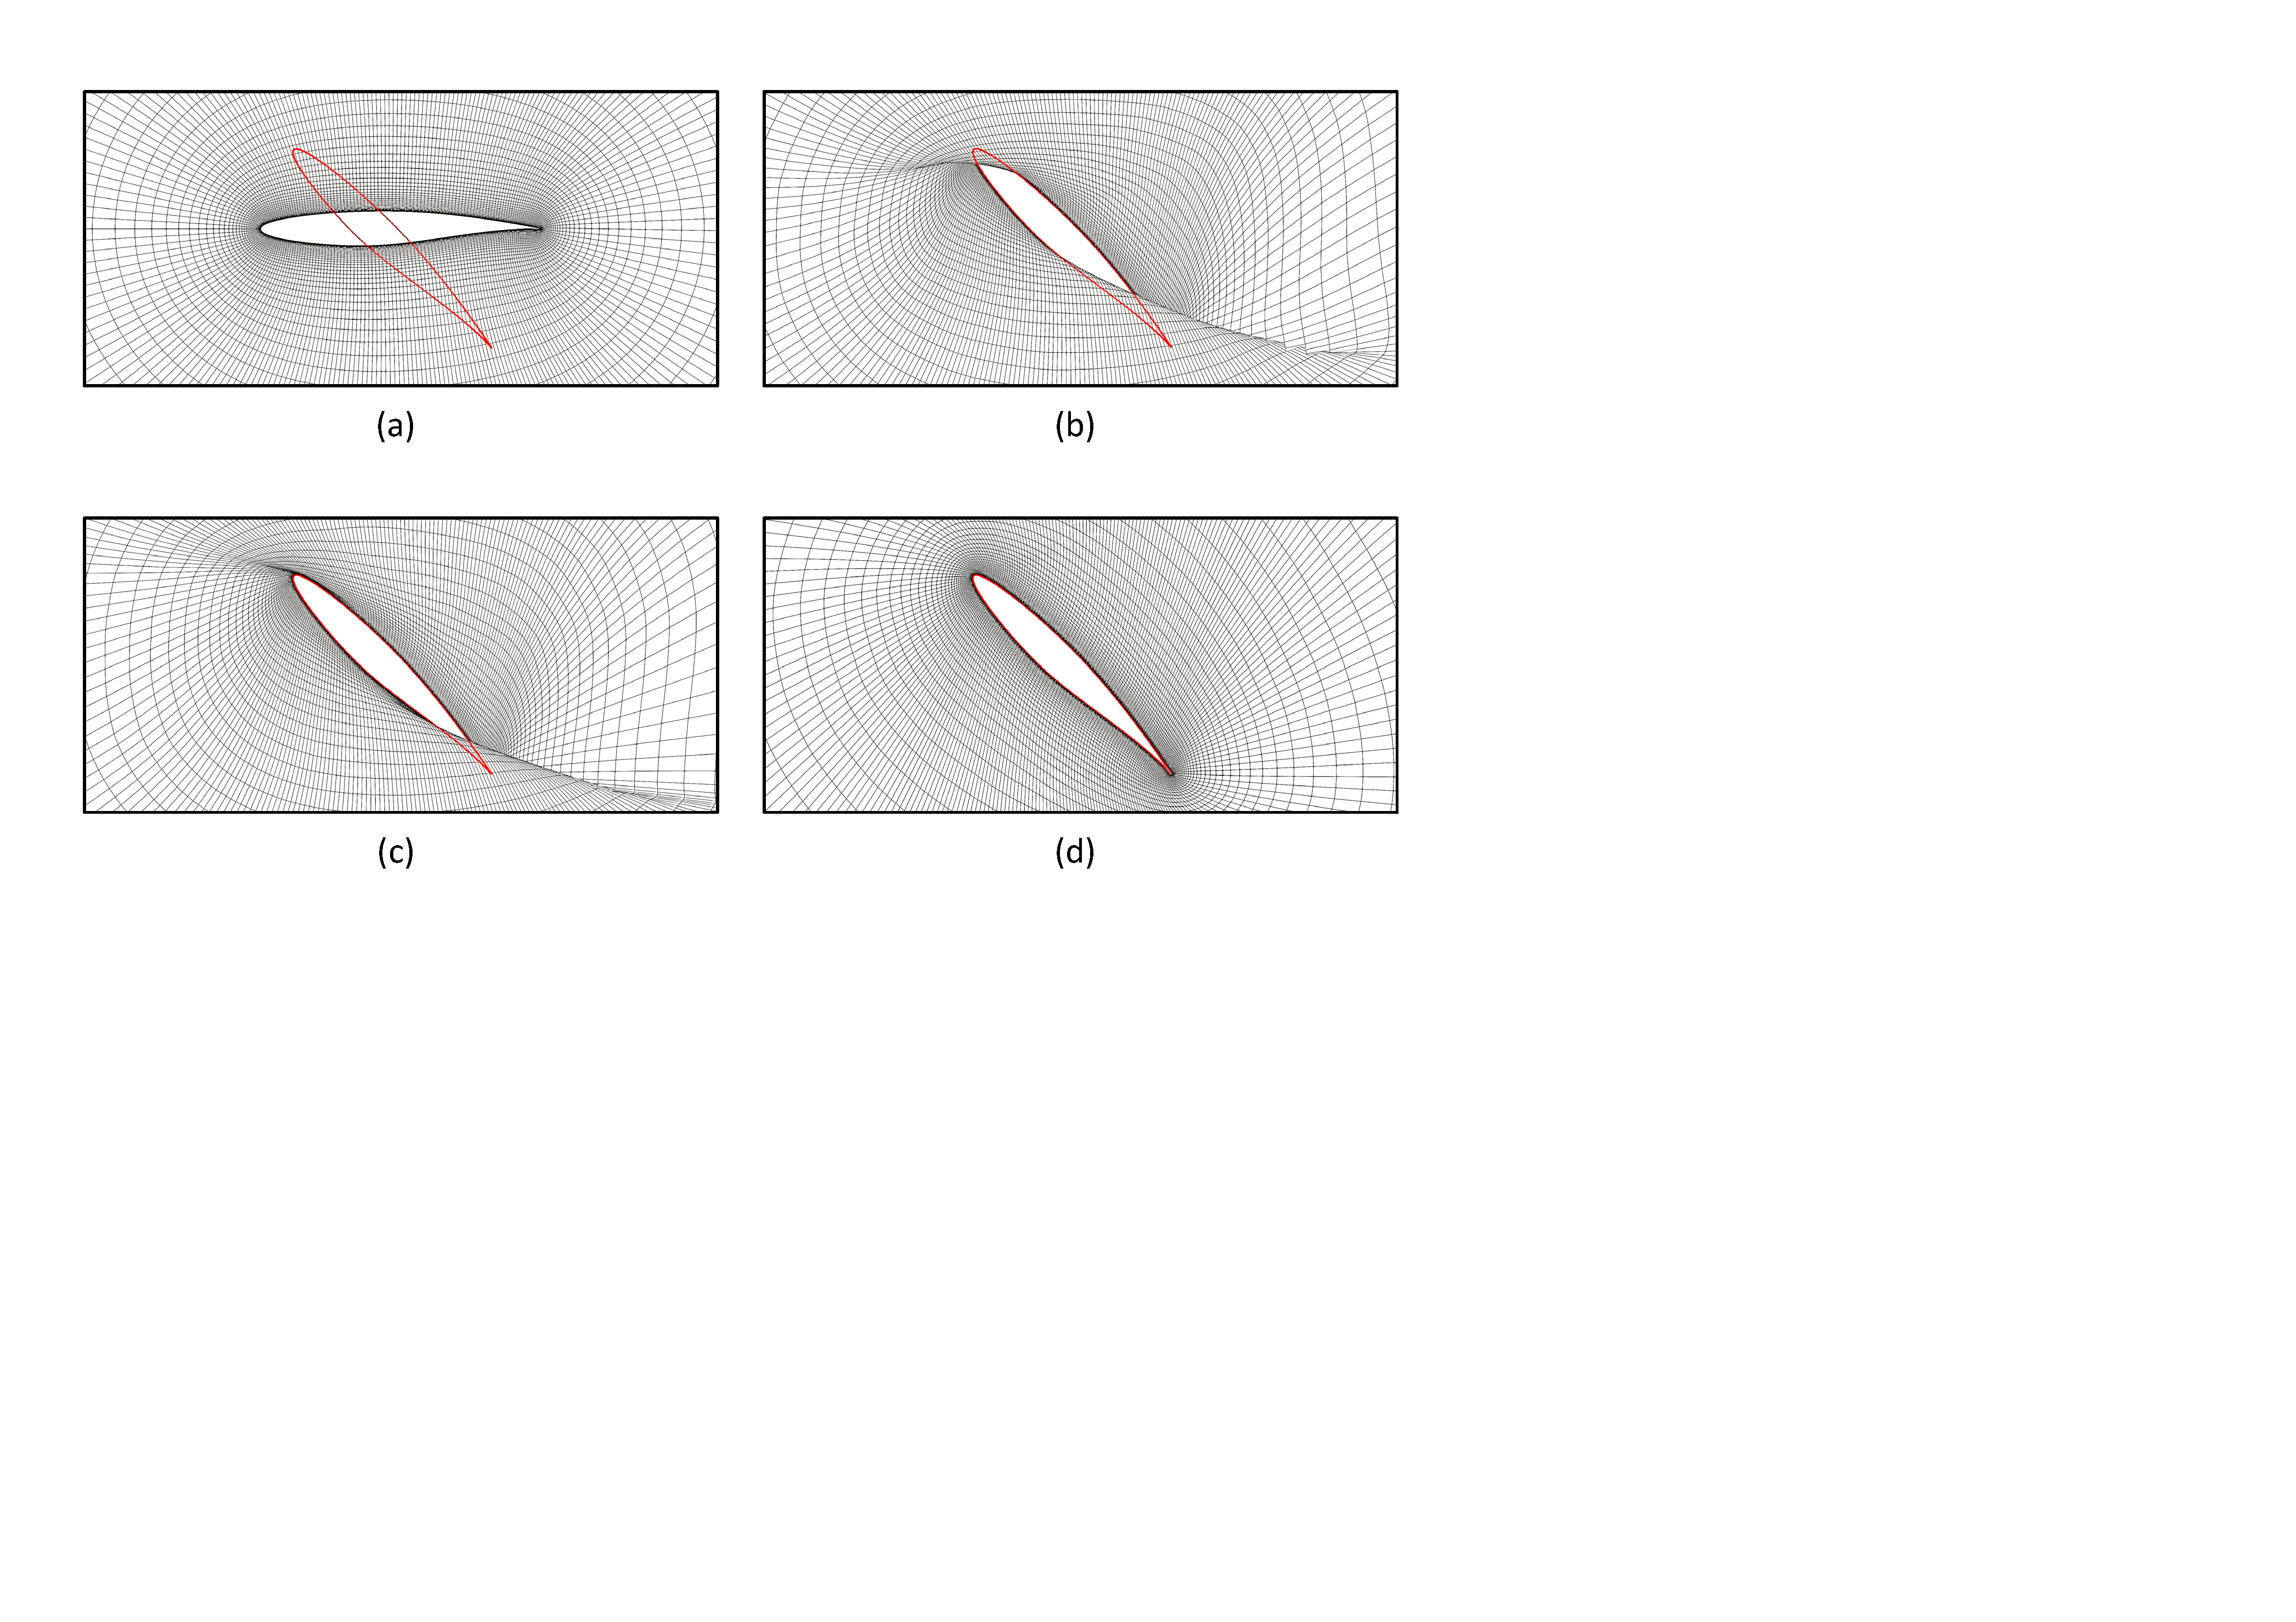
\includegraphics[width=1\linewidth]{chapter5/fig/journal_ablation_studies_w_loss_reg.pdf} 
    \end{center}
    \caption{
        \small \textbf{ Investigation of $\cL_{\rm reg}$ by deforming the mesh in black to fit the shape in red, as shown in (a), with (b) $\lambda_{reg}$=0, (c) $\lambda_{reg}$=10 and (d) $\lambda_{reg}$=100.}
        %Effectiveness of the regularization}  $\cL_{\rm reg}$. 
        %(a) The investigation starts with the template mesh $\hat{M}$ in black and the target shape $S$ in red. 
        %(b) It shows deformation without regularization ($\lambda_{reg}$=0). Severe mesh issues such as overlapped cells and high nonorthognality appear.
        %(c) With $\lambda_{reg}=10$, the mesh quality improves.
        %(d) With $\lambda_{reg}=100$, the mesh issues are removed and the deformed mesh has comparable quality for simulation as that of the original template mesh.
    }
    \label{ch5:fig:w_loss_reg_ablation}
\end{figure}

%-------
% OLD
%--------

\iffalse

The $\cL_{\rm reg}$ implements an isometric mapping of $\mathbb{R}^3 \rightarrow \mathbb{R}^3$ by developing from the 
The goal of HLLE model is to reconstruct a mapping such that the Hessian vanishes at the input coordinates. 
This vanishing Hessian guarantees the mapping outputs the isometric coordinates in the deformed space, preserving the local geometric structure of the manifold.
To this end, we regard the input template CFD mesh as a discretization of an isotropic Euclidean coordinate space.
The tangent space is identical to the input coordinate space itself.
DeepGeo's Hessian at an arbitrery position $\bv$ can be efficiently calculated with the Cartesian coordinate system, defined as
\begin{small}
\begin{align}
       \bH \left( \bv \right) 
      = \begin{bmatrix}
            \frac{\partial^2 \bv}{\partial x^2} & \frac{\partial^2 \bv}{\partial xy} &  \frac{\partial^2 \bv}{\partial xz} \\
            \frac{\partial^2 \bv}{\partial xy} & \frac{\partial^2 \bv}{\partial y^2} &  \frac{\partial^2 \bv}{\partial yz} \\
            \frac{\partial^2 \bv}{\partial xz} & \frac{\partial^2 \bv}{\partial yz} &  \frac{\partial^2 \bv}{\partial y^2} \\
        \end{bmatrix}
\label{ch5:eq:L_reg} 
\end{align}
\end{small}
, DeepGeo relies on a loss term that minimizes the quadratic form of Hessian as $\int_{\mathfrak{C}} \left\| \bH(\mathit{c})) \right\|^2_F d\mathit{c}$, where $\mathfrak{C}$ is the subset of input coordinate space bounded by $\hat{V}^V$ that defines the CFD computational domain.
This quadratic term measures DeepGeo's average ‘curviness’ over $\mathfrak{C}$.
Thanks to neural network's generalization ability, $\cL_{\rm reg}$ can effectively implement the quadratic form of Hessian by only sampling a finite and small number of vertices from $\hat{V}^V$, resulting in the form as in Eq.\ref{ch5:eq:losses}.
\WZ{Let me know if a small ablation study is still needed.}

\fi

\subsubsection{Implementation Details}
\label{ch5:sec:implement}

DeepGeo is implemented as a multi-layer perceptron (MLP) model, with three-dimensional input and output layers.
For 2D ASO cases, the $z$ coordinate is simply set to zero.
The default configuration of DeepGeo for all case studies includes three hidden layers with dimensions of 64, 256, and 512 from input to output, respectively.
Each layer includes a bias terms and uses weight normalization~\cite{ai.Salimans2016b}, resulting in a total of $151,686$ parameters. 
While this amount of weights appears large, it does not directly reflect DeepGeo’s actual model complexity, which is much smaller than what the raw number of weights might indicate. We provide a detailed discussion in Sec.~\ref{ch5:sec:complexity}.
The activation function is a sum of ReLU~\cite{ai.Fukushima1969} and sine functions, which ensures fast convergence and allows for the computation of higher-order derivatives required by $L_\text{reg}$.
During DeepGeo's initialization stage, $\lambda_{fix}=1$ and $\lambda_{reg}=100$ as in Eq.~\ref{ch5:eq:weight_init_expanded}.
DeepGeo employs the same configuration across all cases discussed in Section~\ref{ch5:sec:cases}, without any further tuning.

When a computational mesh associated with the target surface $S$ is available, it can be used as the template CFD mesh $\hat{M}$. 
In this case, the minimization of Eq.~\ref{ch5:eq:weightInit} reduces to learning zero deformations, a process we name the self-initialization. 
A straightforward approach might be to initialize all network weights to zero, but this would prevent further optimization since all gradients would also be zero. Instead, we initialize the network randomly and train it to approximate zero deformations. Experience shows that this does not result in a trivial solution and allows further optimization.



\subsection{Adjoint-Based Shape Optimization with Deep Geometric Mapping Model}
\label{ch5:sec:adj}

For all ASO case studies discussed in this paper, the DeepGeo model is coupled with the finite-volume CFD solver ADflow~\cite{aa.Mader2020} for Reynolds-Averaged Navier-Stokes (RANS) simulation using the Spalart–Allmaras (SA) turbulence model, based on the generated CFD mesh $M$ from DeepGeo.
Sensitivities of optimization objectives with respect to the object surface $V^S$ are obtained with ADflow's discrete adjoint solver.
Meanwhile, the deformed object surface is evaluated according to the geometric constraints, denoted as $L_\text{cons}$.
The value of $L_\text{cons}$ corresponds to the optimization infeasibility.
These constraints are implemented as differentiable soft constraints, and their gradients with respect to $V^S$ are calculated via auto-differentiation.
The gradients of $\Theta$ are then computed by applying the chain rule that begins with the ADflow's surface sensitivities and the gradients of geometric constraints. The RAdam~\cite{ai.Liu2020h} optimizer is used to update $\Theta$.

The overall objective function is formulated as:
%
\begin{equation}
    \cO = \cO_{\rm CFD} + \lambda_{\text{cons}}L_{\rm cons} + \lambda_{\text{reg}}\cL_{\rm reg} + \lambda_{\text{fix}}\cL_{\rm fix}\;, \label{ch5:eq:asoObj}
\end{equation}
%
where $\lambda_{fix}=1$ and $\lambda_{reg}=0.1$. $\lambda_{\text{cons}}$ is a balancing weight that depends on the number, dimension, and unit of different geometric constraints. 
The regularization loss $\cL_{\rm reg}$ and the fixed loss $\cL_{\rm fix}$ are as defined in  Eq.~\ref{ch5:eq:losses}, and the loss weights $ \lambda_{\text{reg}}$ and  $\lambda_{\text{fix}}$ remain constant. 
These losses help preserve CFD mesh quality and ensure fixed patches remain unchanged during optimization.
$O_{\text{CFD}}$ represents physical objectives, such as minimizing drag or maximizing lift. 
It is defined precisely, along with $L_\text{cons}$, in each case study below. 
ASO then involves finding the solution to:
%
\begin{align}
    \Theta^* &=  \argmin_{\Theta} \left(
        \cO\left(F_{\Theta}(\ Vassberg08{V}), \Theta\right)
    \right) \nonumber \\
    &= \argmin_{\Theta} \left(
        \cO_{CFD}\left(\left\{\hat{V} + F_{\Theta}(\hat{V}), E\right\}\right) 
        + w_{cons}L_{\rm cons} \left( \Theta \right)
        + \lambda_{\rm reg} \cL_{\rm reg} \left(\Theta \right)
        + \lambda_{\rm fix}  \cL_{\rm fix} \left(\Theta \right)
    \right)
    \; ,
\end{align}
%
where $\left\{ \hat{V} + F_{\Theta}(\hat{V}) \right\}$ denotes the set of vertices displaced by the translations predicted by $f_{\Theta}$. This iterative process is terminated using an early stopping strategy, a common approach in gradient-descent-based neural network training~\cite{ai.Morgan1989}, which stops the process when $O$ reaches a user-defined threshold or shows no significant improvement after a certain number of iterations.

DeepGeo's configuration remain fixed across different ASO applications, making it a tuning-free and fully automatic parameterization. In the following sections, the effectiveness of DeepGeo-based ASO framework is verified through three different case studies, including optimizing a 2D circle, a 3D business jet wing, and a 3D Blended-Wing-Body aircraft.
\section{Case Studies of Aerodynamic Shape Optimization}
\label{ch5:sec:cases}

In this section, we demonstrate the versatility of our approach in three distinct cases: minimizing drag from a 2D circle, optimizing the NASA's Common Research Model Wing~\cite{aa.Vassberg2008}, and optimizing a Blended-Wing-Body aircraft~\cite{aa.Liebeck2004}. Despite the substantial differences between these cases, we apply the same configuration for all 2D and 3D cases without any fine-tuning. This fixed configuration highlights the ease of using DeepGeo compared to the state-of-the-art FFD-based method, which we use as a baseline for comparison. Unlike FFD, our approach requires no careful configuration of control points across cases, eliminating the need to determine their number and positions, constrain the value ranges of design variables, or develop global design functions. Configuring FFD for different tasks and geometries is time-consuming, demands extensive expertise, and often relies on trial-and-error.
\subsection{Optimization Starting from a Circle}
\label{ch5:sec:cs1}

We first study the case of a 2D circle , which we aim to optimize to minimize drag, with the expectation that it will naturally converge toward the shape of a supercritical airfoil. This case involves significant geometric deformations, testing DeepGeo’s ability to maintain global shape smoothness while allowing large deformation freedom and ensuring robust mesh deformation under challenging conditions.

\subsubsection{Problem Formulation}

We begin with a 2D circle of diameter one and apply the same experimental setup as in the ADODG-2 transonic airfoil optimization benchmark~\footnote{\url{https://sites.google.com/view/mcgill-computational-aerogroup/adodg}}. The objective is to minimize the drag coefficient $C_D$ while maintaining the lift coefficient $C_L$ at $0.824$ and constraining the pitching moment coefficient to $C_M \geq -0.092$. The optimization is performed in a transonic turbulent flow with a Mach number of $0.734$, a Reynolds number of $5\times 10^6$ and an initial angle of attack of $2.0^{\circ}$. 
We used pyHyp~\cite{aa.Secco2021} to compute the CFD template mesh shown in Fig.~\ref{ch5:fig:cs1_template_mesh}(a), which comprises $20,331$ cells.

\begin{table}[htb]
  \centering
  \caption{\small Aerodynamic shape optimization task specifications for the Case Study I.}
  \resizebox{0.95\columnwidth}{!} {
        \begin{tabular}{lllrr}
        \hline
        \multicolumn{1}{l}{\textbf{Objectives}} & \textbf{Functions/Variables} & \textbf{Description} & \multicolumn{1}{l}{\textbf{DeepGeo Quantity}} & \multicolumn{1}{l}{\textbf{FFD Quantity}} \\
        \hline
        \multicolumn{1}{l}{\textbf{Minimize}} & $C_D$  & Drag coefficient &        &  \\
        \hline
        \multicolumn{1}{l}{\multirow{3}[2]{*}{\textbf{With respect to}}} & $\Theta$ & Weights of DeepGeo & \num{151585} &         \\
        \multicolumn{1}{l}{} & $P_z$  & Control points' $z$ coordinates &        & 30 \\
        \multicolumn{1}{l}{} & $\alpha$ & Angle of attack & 1      & 1 \\
        \hline
        \multicolumn{3}{l}{\textbf{Total design variables}} & \num{151586} & 31 \\
        \hline
        \multicolumn{1}{l}{\multirow{6}[2]{*}{\textbf{Subject to}}} & $C_L=0.824$ & Lift coefficient constraint & 1      & 1 \\
        \multicolumn{1}{r}{} & $C_M\leq0.092$ & Moment coefficient constraint & 1      & 1 \\
        \multicolumn{1}{r}{} & $t \ge 0.2\,t_\text{RAE2822}$ & Minimum thickness constraints &        & 30 \\
        \multicolumn{1}{r}{} & $A \ge 0.0654$ & Minimum area constraints &   1    &  1 \\
        \multicolumn{1}{r}{} & $\delta \bv^\text{TE}=0$ & Trailing edge constraint & 1      &  \\
        \multicolumn{1}{r}{} & $\delta \bv^\text{LE}=0$ & Leading edge constraint & 1      &  \\
        \multicolumn{1}{r}{} & $0.5 \leq \alpha \leq 4.0$ & Angle of attack constraint & 1      &  1 \\
        \hline
        \multicolumn{3}{l}{\textbf{Total constraints}} & 6      & 34 \\
        \hline
        \multicolumn{3}{l}{\textbf{Need value range limits for each DV?}} & NO     & YES \\
        \hline
        \end{tabular}%
    }
  \label{ch5:tab:circle_2_airfoil_DV_cons}%
\end{table}%

\begin{figure}[htb]
    \begin{center}
        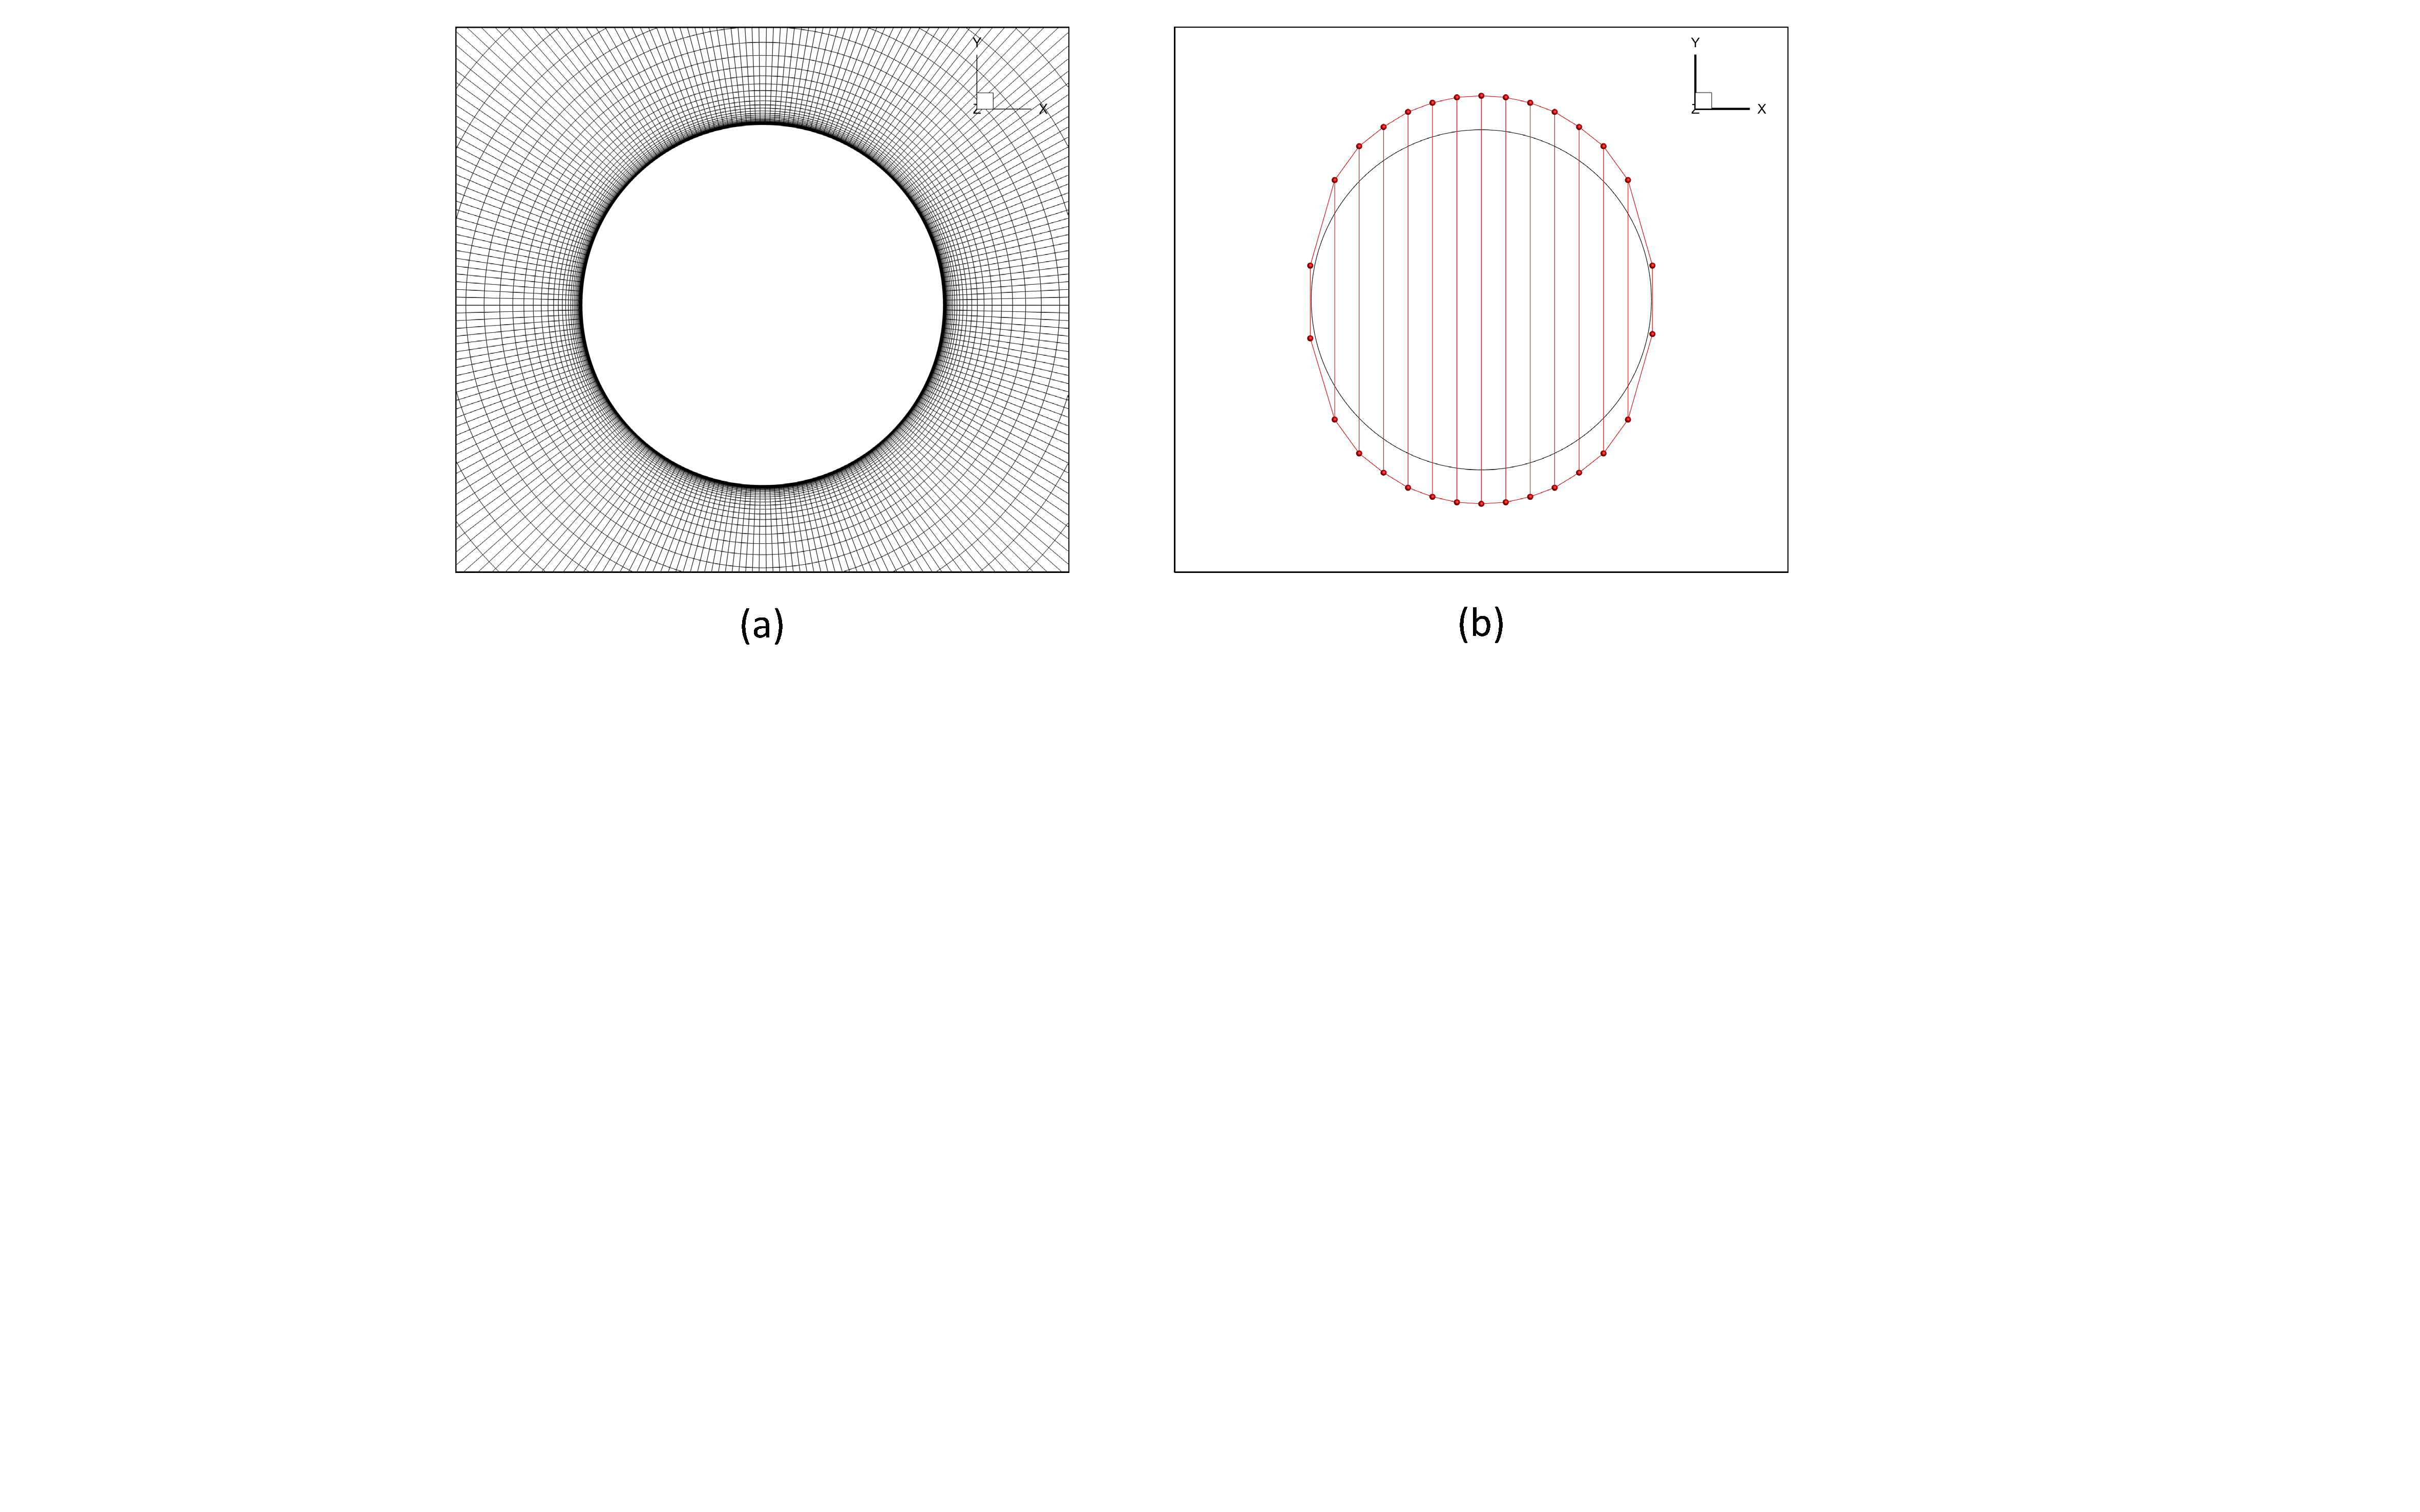
\includegraphics[width=0.8\linewidth]{chapter5/fig/circle2airfoil_template_mesh_initial_geometry.pdf}
    \end{center}
     \vspace{-7mm}
    \caption{
        \small Geometric setup in the 2D airfoil case. (a) DeepGeo template mesh $\hat{M}$. (b) Control points for the FFD baseline.
    }
    \label{ch5:fig:cs1_template_mesh}
\end{figure}

\begin{figure}[htb]
     \begin{center}
         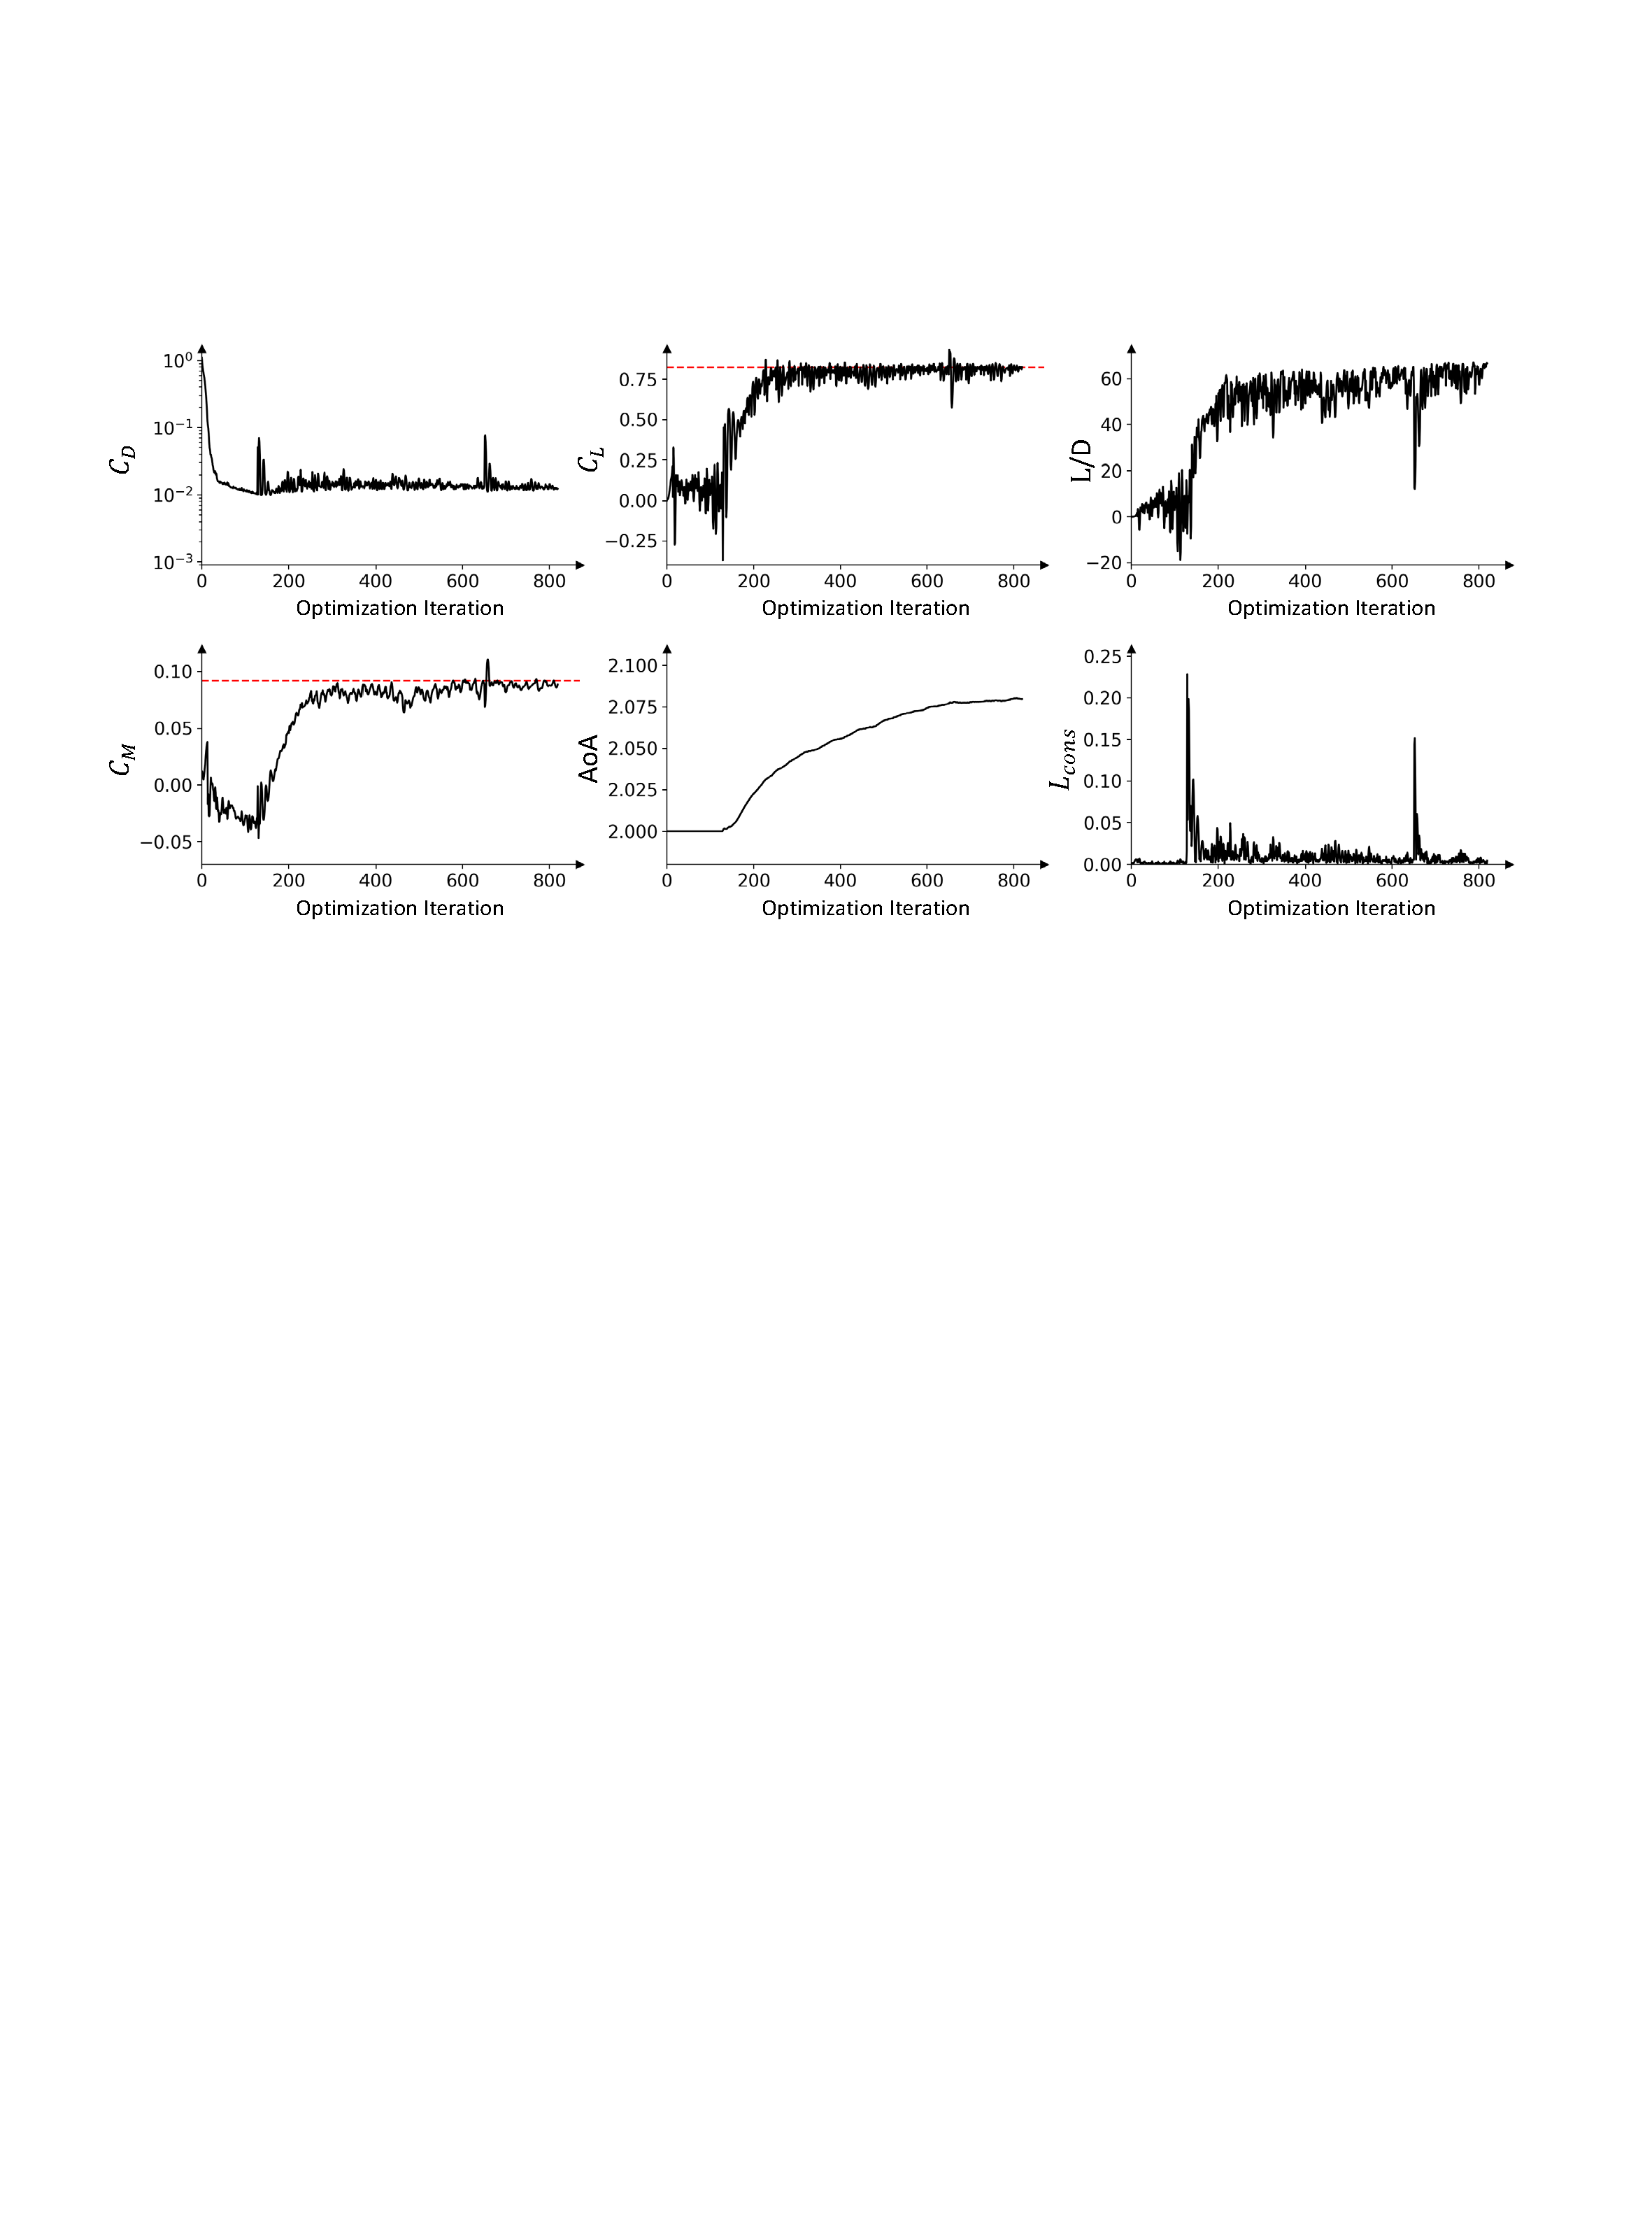
\includegraphics[width=1\linewidth]{chapter5/fig/circle2airfoil_optim_history.pdf}
     \end{center}
      \vspace{-7mm}
     \caption{
         \small Evolution of important quantities during optimization for the 2D airfoil case. The dashed lines in the $C_L$ and $C_M$ plots indicate the target values for these quantities, which are closely approached by the end of the optimization, demonstrating the precision and effectiveness of the DeepGeo model in reaching aerodynamic targets.
     }
     \label{ch5:fig:cs1_history}
 \end{figure}

\begin{figure}[!htb]
    \begin{center}
        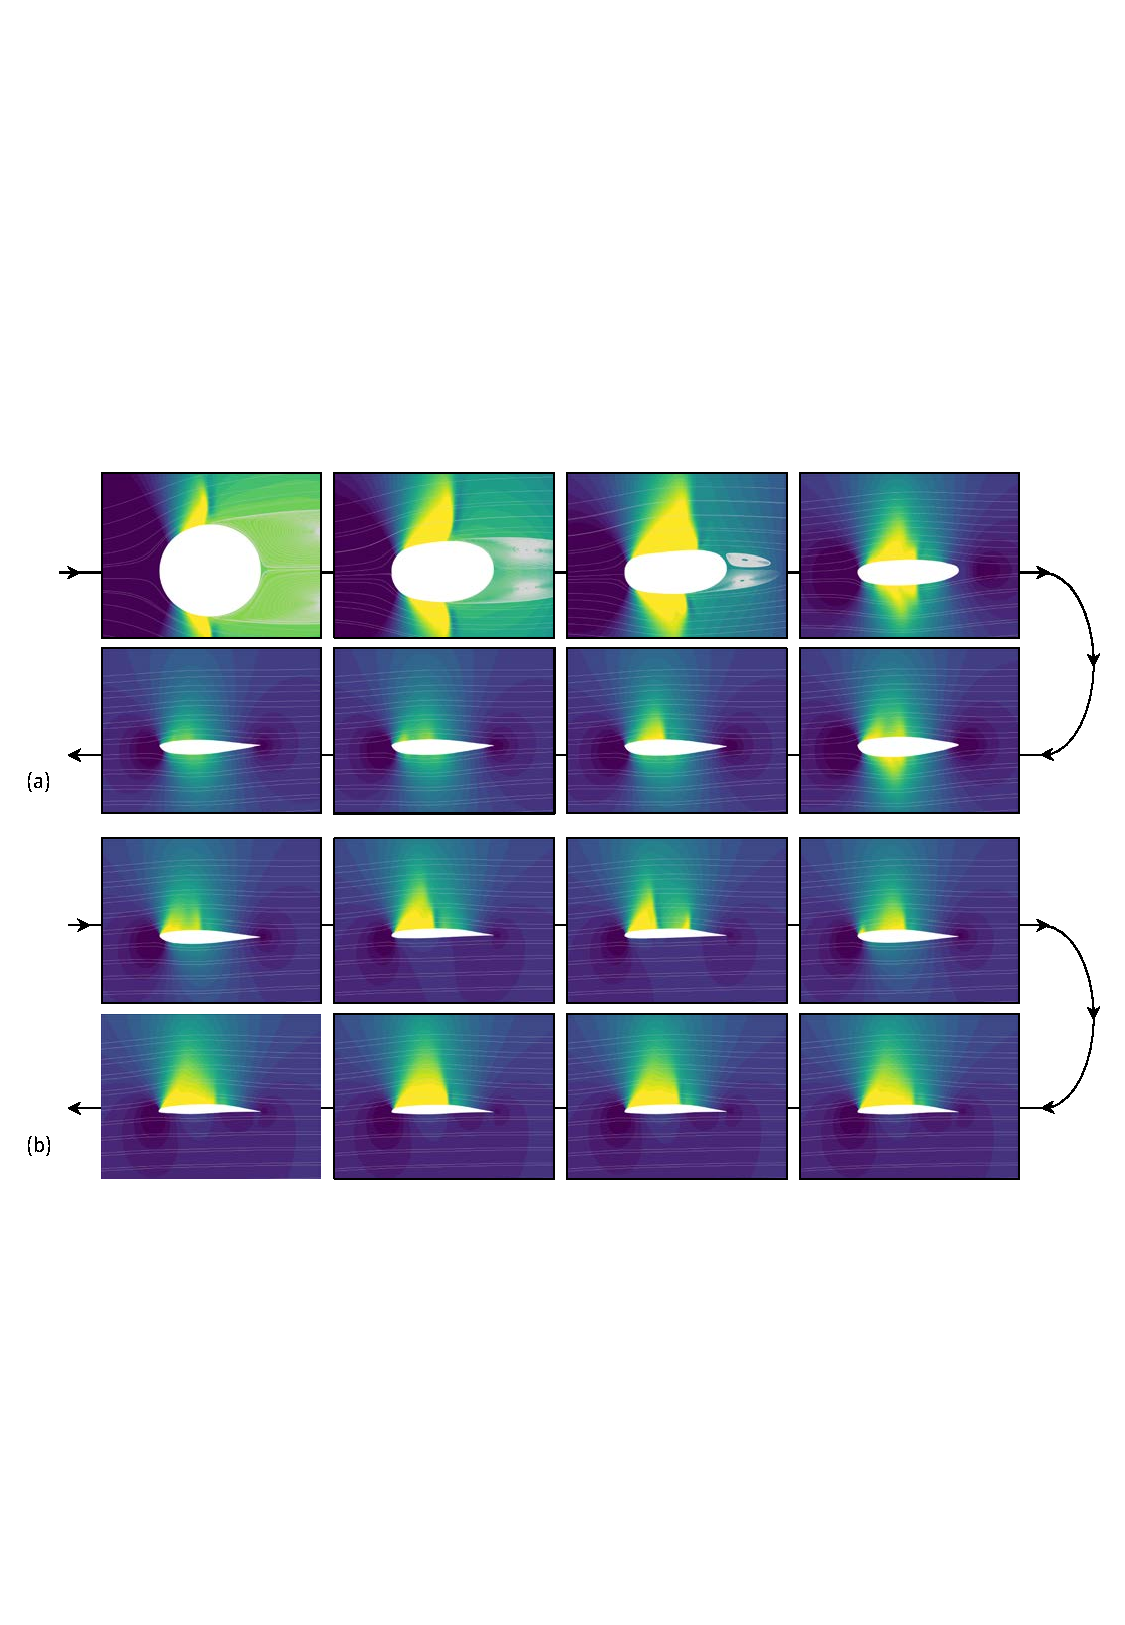
\includegraphics[width=1\linewidth]{chapter5/fig/circle2airfoil_optim_field_visualization.pdf}
    \end{center}
      \vspace{-7mm}
    \caption{
        \small  Evolution of the pressure coefficient field in the 2D airfoil case.  (a) Minimizing $C_D$ alone. (b) Minimizing $C_D$ while setting a target for $C_L$ and $C_M$.
    }
    \label{ch5:fig:cs1_cp}
\end{figure}

\subsubsection{Configuring DeepGeo}

Following the same optimization strategy proposed in~\citet{aa.Li2021}, we perform a two-step optimization. First, the drag coefficient $C_D$ is minimized. Then, terms are added to the objective function to address the lift and moment coefficients, $C_L$ and $C_M$, and the optimization continues. For this purpose, two versions of the function $ \cO_{CFD}$ from Eq.~\ref{ch5:eq:asoObj} are defined to represent the physical objectives as:
%
\begin{align}
    &\cO_{CFD,1} = \left| C_D \right|\;, \\
    &\cO_{CFD,2} = \left| C_D \right| + \left| C_L-0.824 \right| + \max \left( -0.092 - C_M, 0 \right) \;, \nonumber 
\end{align}
%
where the coefficients are obtained with the adjoint solver (denoted as $g$) as $(C_D,C_L,C_M)=g\left(\{\hat{V}+F_\Theta(\hat{V}),E\}\right)$. 
We use the Shoelace formula to compute deformed airfoil's area $A(V^S)$. The geometric loss $\cL_{cons}$ includes a term that constrains the area from falling below the RAE 2822 profile area (\num{0.0654}), along with two additional terms that fix the leading and trailing edge vertices (LE and TE), respectively. This is expressed as:
 %
\begin{equation}
    \cL_{cons} = 
    \underbrace{\max {(0.0654-A(V^S),0)}^2}_\text{area constraint} + 
    \underbrace{\left|\left| \delta\bv^\text{LE} \right|\right|^2}_\text{LE constraint} + 
    \underbrace{\left|\left| \delta\bv^\text{TE} \right|\right|^2}_\text{TE constraint}\;.
\end{equation}
%
As discussed in Section~\ref{ch5:sec:implement}, we use the initial mesh as the template mesh $\hat{M}$.  Tab.~\ref{ch5:tab:circle_2_airfoil_DV_cons} summarizes our experimental setup. 

\begin{figure}[ht]
    \begin{center}
        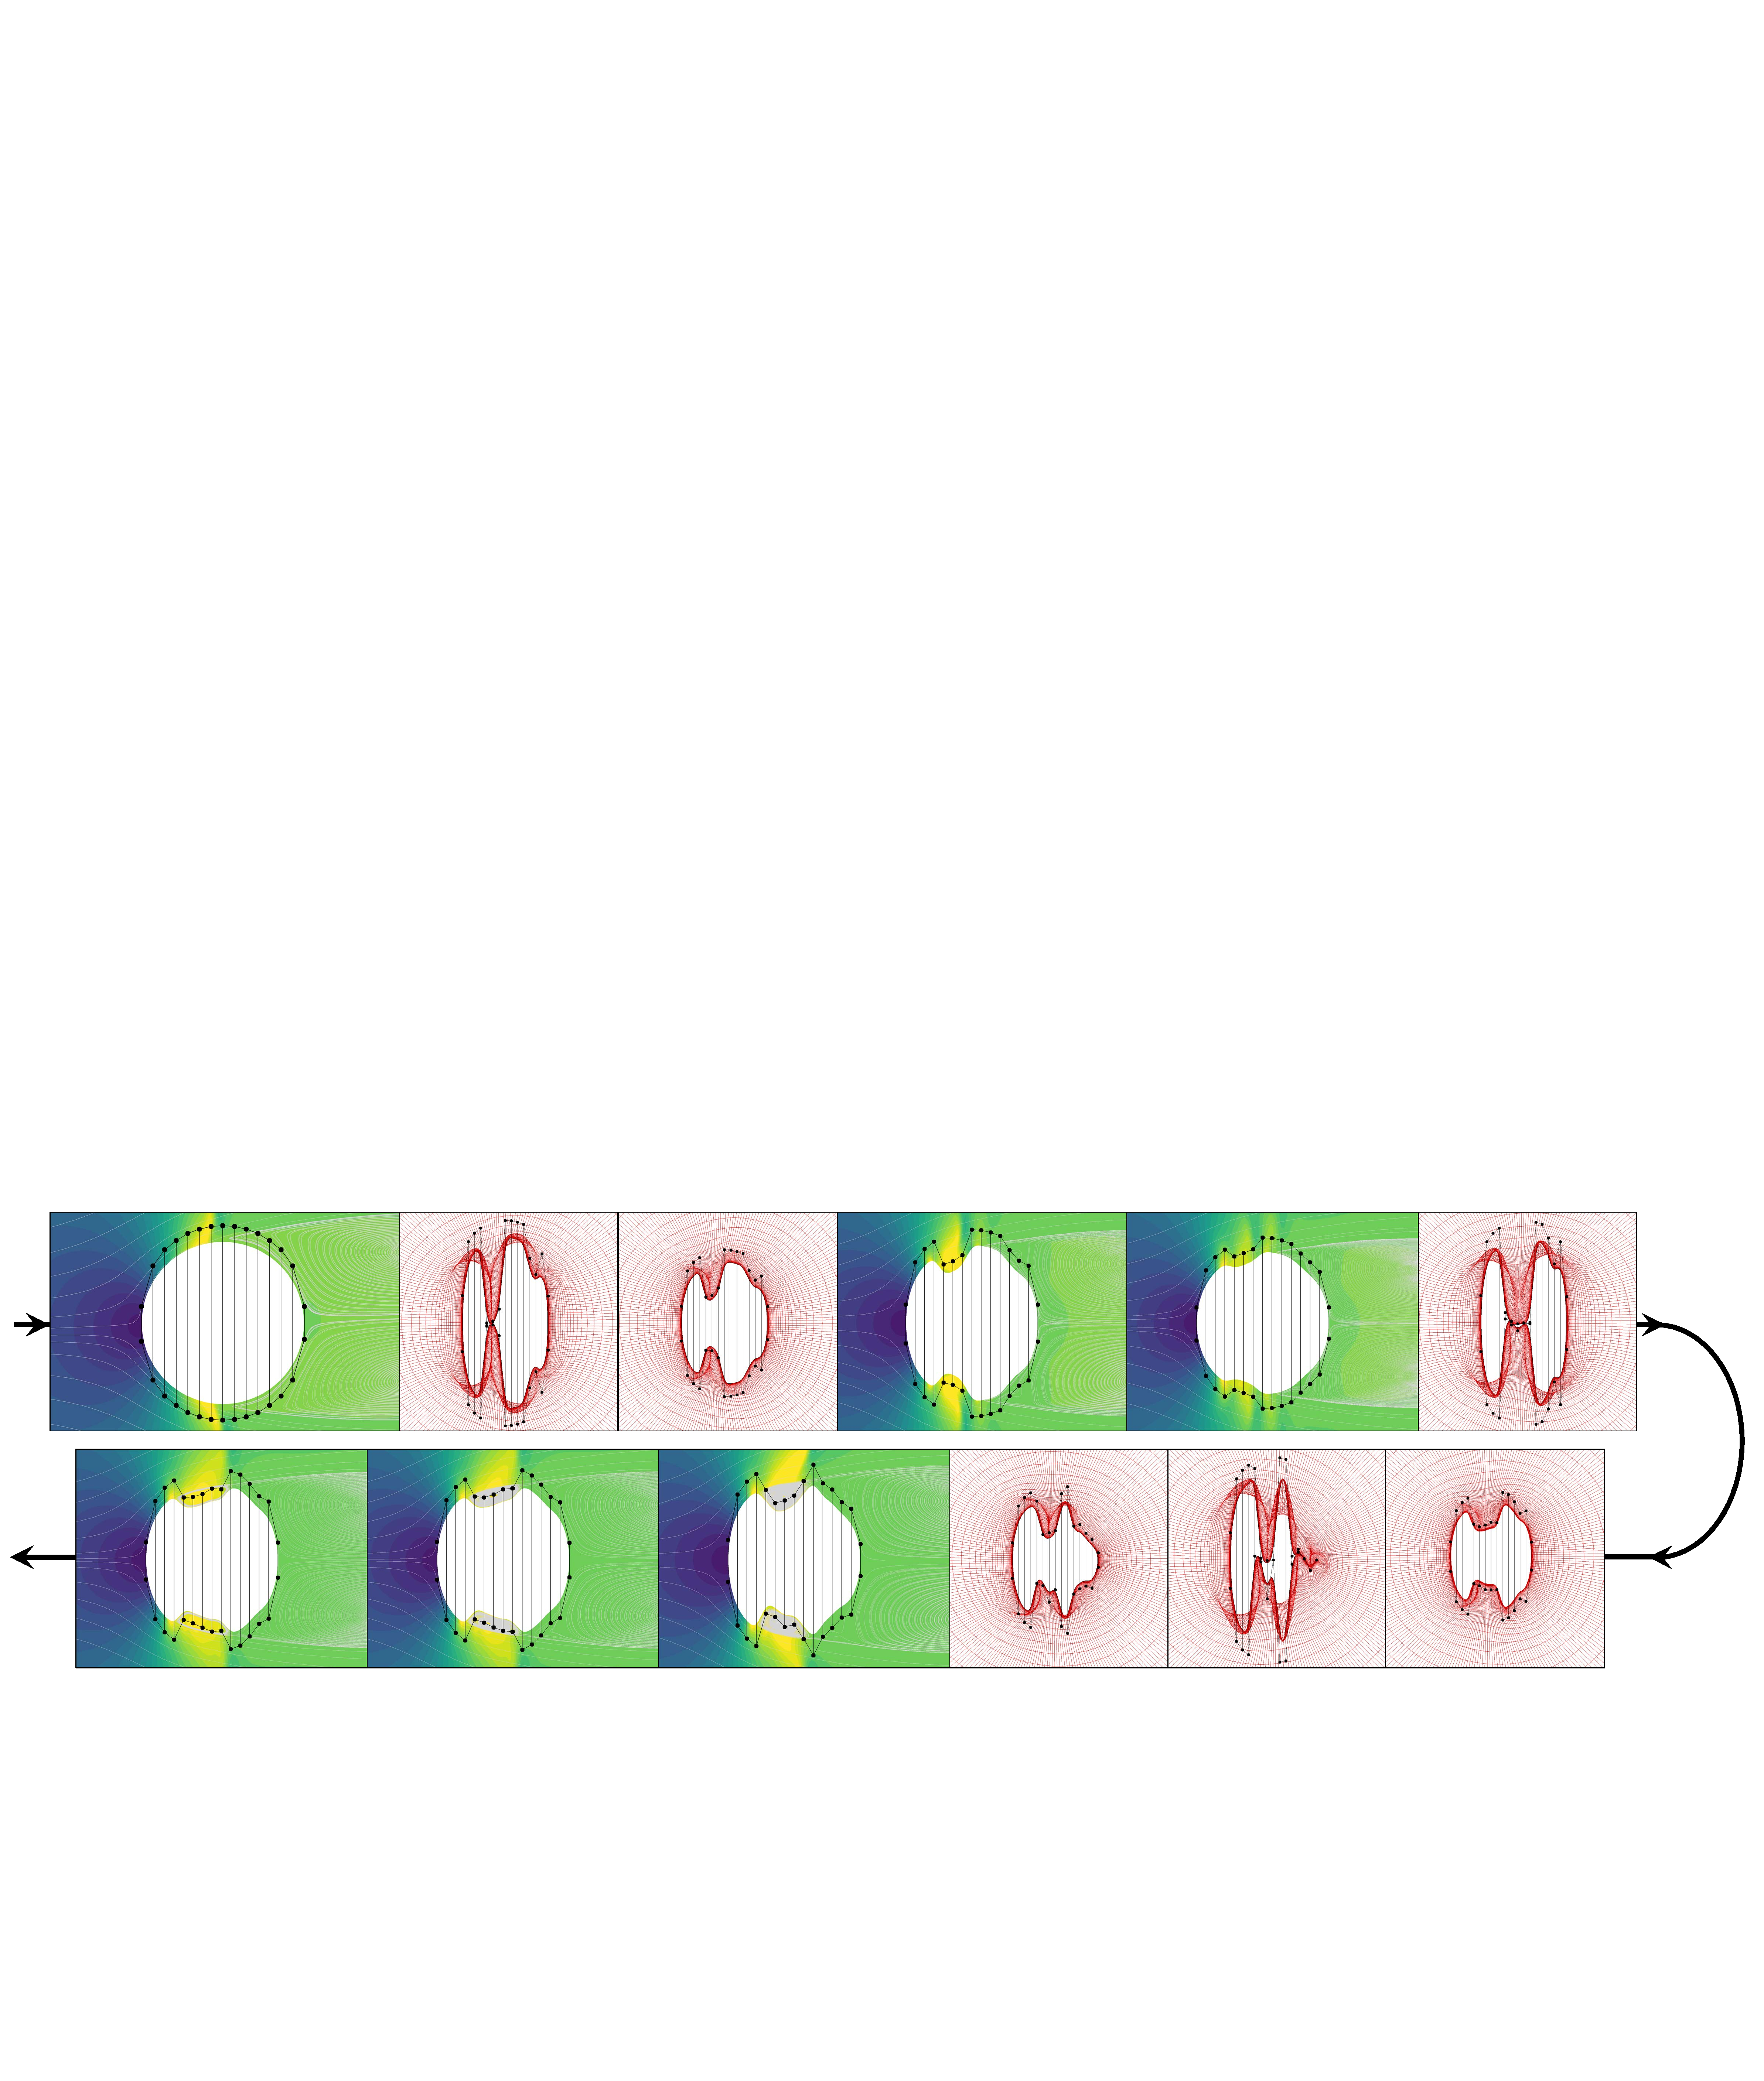
\includegraphics[width=1\linewidth]{chapter5/fig/circle2airfoil_ffd_optim_field_visualization.pdf}
    \end{center}
     \vspace{-7mm}
    \caption{
        \small Failing FFD-based optimization in the 2D airfoil case. The absence of a colored fluid field denotes a simulation that did not converge.
    }
    \label{ch5:fig:cs1_ffd_cp}
\end{figure}

\subsubsection{Configuring the Free-Form Deformation Baseline}

For comparison purposes, we use the implementation of~\cite{aa.Li2021} with a 30-point configuration for FFD as shown in Fig.~\ref{ch5:fig:cs1_template_mesh}(b).
Let the airfoil thickness be $t$, and let $t_\text{RAE2822}$ represent the thickness of the RAE-2822 airfoil.
A set of thickness constraints $t \geq 0.2,t_\text{RAE2822}$ is applied to prevent negative volume errors at the beginning of the optimization. The optimization is conducted using the SLSQP optimizer available in pyOptSparse\cite{aa.Wu2020}.

\subsubsection{Results and Analysis}
\label{ch5:sec:circle_2_airfoil_result}

The optimization process is illustrated in Fig.~\ref{ch5:fig:cs1_history}, while the fluid field changes are visualized in Fig.~\ref{ch5:fig:cs1_cp}. When minimizing $\cO_{CFD,1}$, the drag coefficient $C_D$ is reduced significantly by $99.1\%$.
The shape gradually and smoothly becomes thinner, with the leading and trailing edges emerged and symmetry largely preserved. No singular shapes or simulation failures occur, demonstrating the robustness of DeepGeo to large mesh deformations.
In the second stage, symmetry is broken to achieve a streamlined profile commonly observed in high-lift transonic airfoils, effectively generating more lift.
A shock wave initially appears but is gradually diffused, and by the end of the optimization, it largely dissipates.
The final airfoil achieves  $C_D=\num{0.012195}$ (i.e. $121.95$ counts), and its lift-over-drag ratio ($L/D$) is significantly improved from \num{1e-3} to $67.22$, which makes it  comparable to that of modern supercritical airfoils designed for transonic flights. This result validates DeepGeo’s effectiveness in achieving high-performance designs.

In contrast, the FFD-based optimization fails after a small number of iterations due to singularities in the deformed shape, leading to severe meshing issues as shown in Fig.~\ref{ch5:fig:cs1_ffd_cp}. In some iterations, simulation failure occurs, represented by the mesh in red. 
Although FFD ensures local smoothness within a control cage, the free movement of control points can lead to global singularities and geometric abnormalities. These issues persist despite adjustments to the hyperparameters. Such failures do not occur with DeepGeo, highlighting its stability and reliability for complex shape optimizations that require high deformation freedom. 
\subsection{Optimizing the Common Research Model Wing}
\label{ch5:sec:cs2}

We now turn to NASA's Common Research Model Wing (CRM wing), which is extracted from the CRM wing-body configuration. As shown in Fig.~\ref{ch5:fig:cs2_template_mesh}(b), the initial geometry is a 3D wing with a blunt trailing edge. As in the previous case, results are compared to those obtained with the FFD baseline.

\subsubsection{Problem Formulation}

The objective is to minimize the drag coefficient $C_D$ while maintaining a lift coefficient $C_L$ of $0.5$ and ensuring that the pitching moment coefficient $C_M$ is at least $-0.17$. This single-point optimization problem is conducted under fully turbulent flow conditions, with a Mach number of $0.85$, a Reynolds number of $5 \times 10^6$, and an initial angle of attack of $2.2^{\circ}$. Additional constraints require the wing's volume to remain at least as large as its initial value, and its thickness to be no less than $25\%$ of the initial thickness. The trailing edge (TE) vertices and the leading edge (LE) vertex on the root section are fixed, while the remaining LE vertices are restricted to movement along the $z$ direction, preserving the projected area.
The optimization objectives and flow conditions follow the ADODG-4.1 single-point optimization benchmark~\footnote{\url{https://sites.google.com/view/mcgill-computational-aerogroup/adodg}}.

The optimization is performed on a grid with $450,560$ cells, as shown in Fig.~\ref{ch5:fig:cs1_template_mesh}(a), which corresponds to the L2 grid defined in~\citet{aa.Lyu2015}. In this setup, the DeepGeo weights affect only the wing’s surface shape, while the angle of attack is treated as a standalone design variable. Tab.~\ref{ch5:tab:crm_DV_cons} summarizes the experimental setup.

\begin{figure}[!tb]
    \begin{center}
        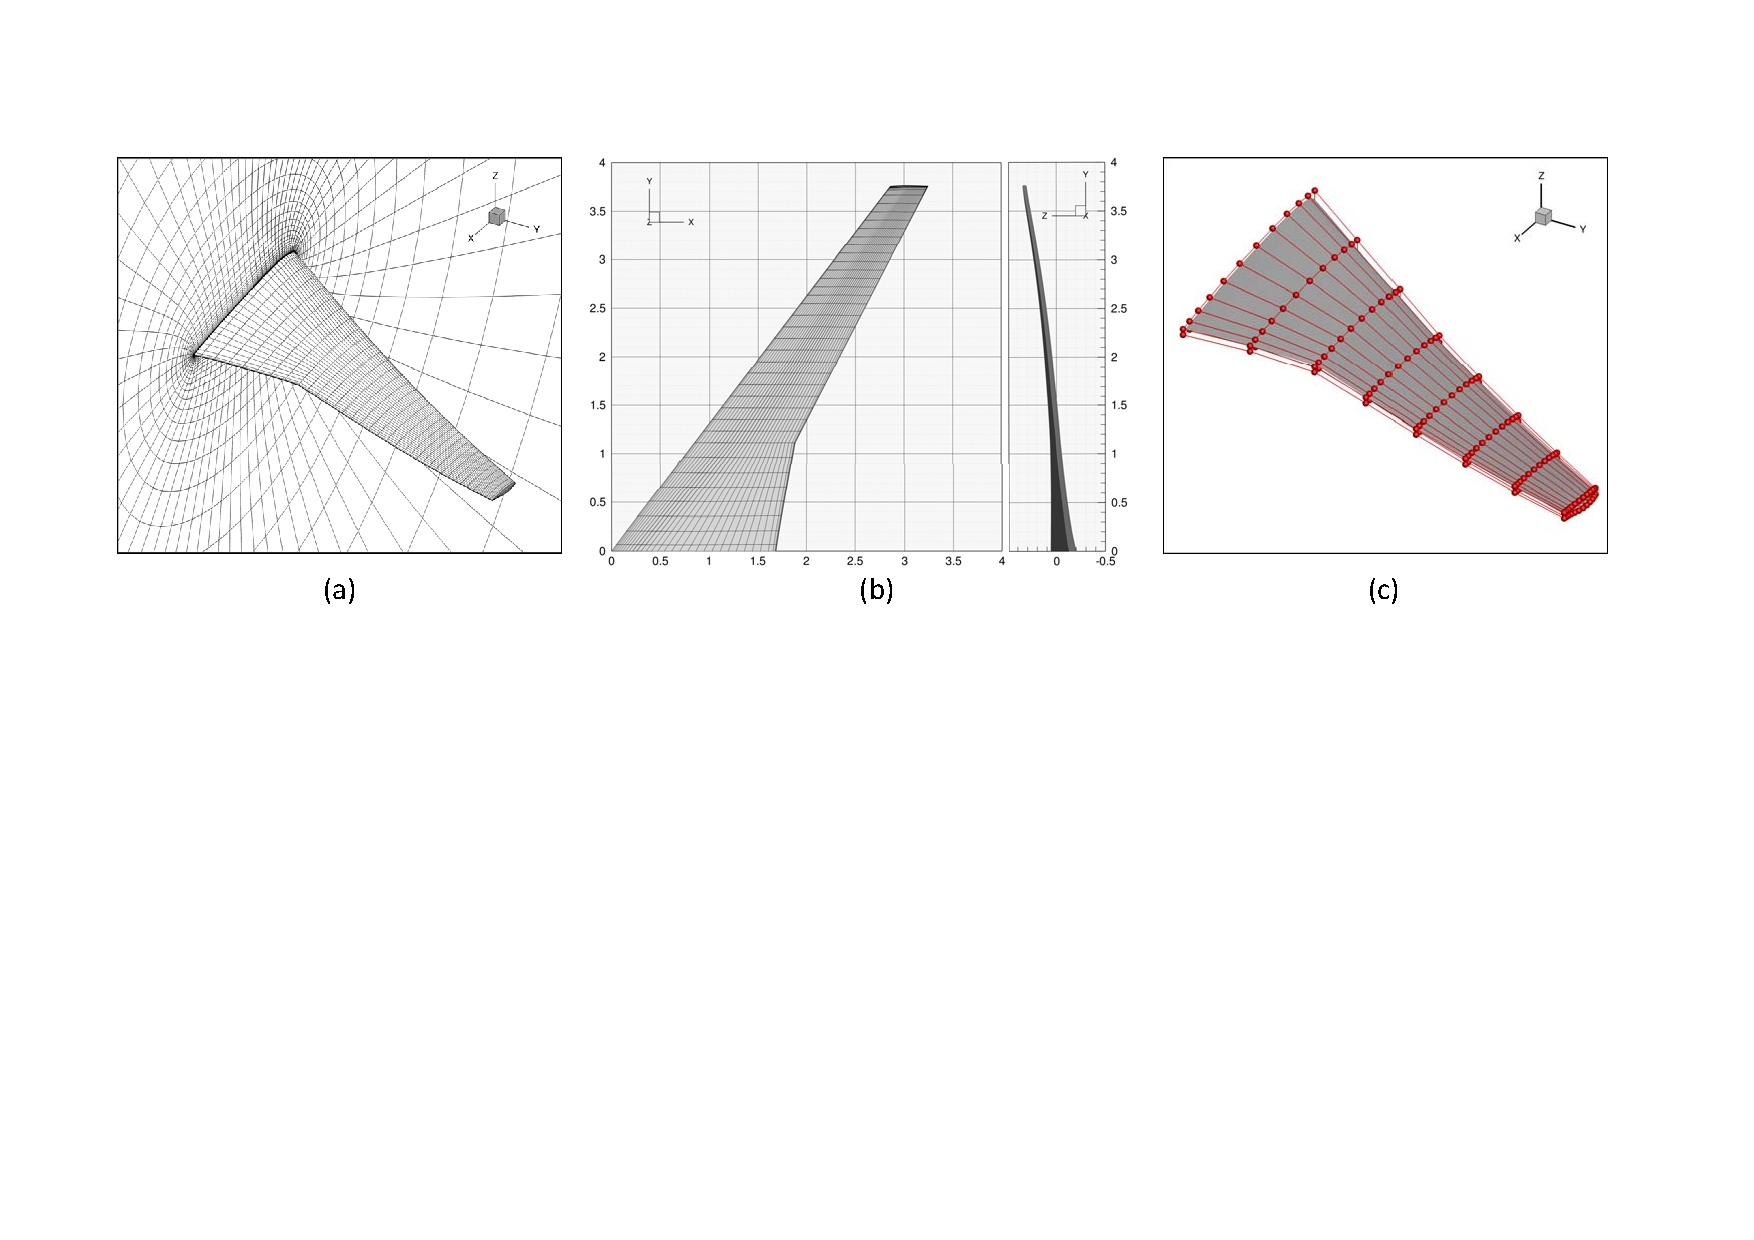
\includegraphics[width=1\linewidth]{chapter5/fig/crm_template_mesh_initial_geometry.pdf}
    \end{center}
    \caption{
        \small The geometric setups for Case Study II, including: (a) the template mesh for DeepGeo, (b) the initial CRM wing geometry and (c) the 192-point FFD setting.
    }
    \label{ch5:fig:cs2_template_mesh}
\end{figure}

\subsubsection{Configuring DeepGeo}

As in the previous case study, the L2 grid is used as the input template mesh $\hat{M}$.
The objective function $\cO_{CFD}$ and the loss function $\cL_{cons}$ from Eq.~\ref{ch5:eq:asoObj} are defined as:
%
\begin{align}
    \cO_\text{CFD} & = \left| C_D \right| + \left| C_L-0.5 \right| + \max \left( -0.17 - C_M, 0 \right) \;, \label{ch5:eq:cfdWing}  \\
    \cL_{cons} & = 
    \underbrace{{\max \left(Vol(V^S)-{Vol}_\text{original}(S), 0\right)} ^2}_\text{volume constraint} + 
    \underbrace{\left|\left|\Delta V^\text{TE}\right|\right|^2}_\text{TE constraint} +
    \underbrace{\left|\left|\Delta V^\text{LE}_x\right|\right|^2 + \left|\left|\Delta V^\text{LE}_y\right|\right|^2}_\text{LE constraint} +
    \underbrace{\left|\left|\delta \bv^\text{LE,root}\right|\right|^2}_{ \substack{\text{fixed-wing root}\\ \text{incidence constraint}} } \; . \nonumber
\end{align}
%
Minimizing $\cO_{CFD}$ aims to reduce $C_D$, bring $C_L$ close to 0.5, and ensure $C_M$ is greater than or equal to $-0.17$.  The extended Shoelace formula~\cite{aa.Zhang2001} is applied to compute the volume $Vol(V^S)$ of the deformed wing, with an arbitrary reference point on the root section plane. ${Vol}_\text{original}(S)$ represents wing's initial volume. The term $\bv^\text{LE,root}$ corresponds to the single leading-edge (LE) vertex on the root section, while $V_x$ and $V_y$ refer to the sets of $x$ and $y$ vertex coordinates, respectively. In practice, DeepGeo satisfies the thickness requirement without an explicit loss function term.

\begin{table}[!t]
  \centering
  \caption{\small Aerodynamic shape optimization task specifications for the Case Study II.}
  \resizebox{1\columnwidth}{!} {
        \begin{tabular}{lllrr}
        \hline
        \multicolumn{1}{l}{\textbf{Objectives}} & \textbf{Functions/Variables} & \textbf{Description} & \multicolumn{1}{l}{\textbf{DeepGeo Quantity}} & \multicolumn{1}{l}{\textbf{FFD Quantity}} \\
        \hline
        \multicolumn{1}{l}{\textbf{Minimize}} & $C_D$  & Drag coefficient &        &  \\
        \hline
        \multicolumn{1}{l}{\multirow{3}[2]{*}{\textbf{With respect to}}} & $\Theta$ & Weights of DeepGeo & \num{151585} &         \\
        \multicolumn{1}{l}{} & $P_z$  & Control points' $z$ coordinates &        & 720 \\
        \multicolumn{1}{l}{} &   & Twist function &        & 7 \\
        \multicolumn{1}{l}{} & $\alpha$ & Angle of attack & 1      & 1 \\
        \hline
        \multicolumn{3}{l}{\textbf{Total design variables}} & \num{151586} & 728 \\
        \hline
        \multicolumn{1}{l}{\multirow{9}[2]{*}{\textbf{Subject to}}} & $C_L=0.5$ & Lift coefficient constraint & 1      & 1 \\
        \multicolumn{1}{r}{} & $C_M\geq-0.17$ & Moment coefficient constraint & 1      & 1 \\
        \multicolumn{1}{r}{} & $t \ge 0.25 \; t_\text{original}$ & Minimum thickness constraints &        & 750 \\
        \multicolumn{1}{r}{} & $Vol \ge {Vol}_\text{original}$ & Minimum volume constraint & 1      & 1  \\
        \multicolumn{1}{r}{} & $\Delta V^\text{TE}=0$ & Trailing edge constraint & 1      &  \\
        \multicolumn{1}{r}{} & $\Delta V^\text{LE}_x=0,\;\Delta V^\text{LE}_y=0$ & Leading edge constraint & 1      &  \\
        \multicolumn{1}{r}{} & $\delta\bv^{\text{LE,root}}=0$ & Fixed-wing root incidence constraint & 1      &  \\
        \multicolumn{1}{r}{} & $\Delta P^{\text{TE,upper}}_z = -\Delta P^{\text{TE,lower}}_z$ & Fixed trailing-edge constraints &        & 15 \\
        \multicolumn{1}{l}{} & $\Delta P^{\text{LE,upper,root}}_z =$ & \multirow{2}[1]{*}{Fixed-wing root incidence constraint} & \multirow{2}[1]{*}{} & \multirow{2}[1]{*}{1} \\
        \multicolumn{1}{l}{} &  $\;\;\;-\Delta P^{\text{LE,lower,root}}_z$ &        &        &  \\
        \multicolumn{1}{r}{} & $2.0 \leq \alpha \leq 4.0$ & Angle of attack constraint & 1      &  1 \\
        \hline
        \multicolumn{3}{l}{\textbf{Total constraints}} & 7      & 770 \\
        \hline
        \multicolumn{3}{l}{\textbf{Need value range limits for each DV?}} & NO     & YES \\
        \hline
        \end{tabular}%
    }
  \label{ch5:tab:crm_DV_cons}%
\end{table}%

\subsubsection{Configuring the Free-Form Deformation Baseline}

For comparison, we use the FFD-based baseline with 192-control-point configuration of \citet{aa.Hwang2019,aa.Li2019}, as depicted in Fig.~\ref{ch5:fig:cs2_template_mesh}(c). Let the control points be $P=\{\bp_1, \bp_2,..., \bp_{192}\}$, where each $\bp=\{p_x, p_y, p_z\}$ and their displacements denoted as $\Delta P$. The positions of control points are optimized, and the wing's surface is interpolated within each control cages to enable localized shape changes. Additionally, a global function is implemented to introduce spanwise twisting, with seven rotation angles treated as additional design variables.
The 192 control points are grouped into seven sections along the wingspan and each section is rotated independently.
For this optimization, we use the MACH-Aero framework, where pyGeo~\cite{aa.Kenway2010} implements the FFD parameterization, IDWarp~\cite{aa.Secco2021} deforms the computational mesh and pyOptSparse~\cite{aa.Wu2020} for optimization.

\subsubsection{Results and Analysis}

\begin{table}[!b]
  \centering
  \caption{\small CRM wing optimization results of the Case Study II. One count for $C_D$ equals to $10^{-4}$.}
    \begin{tabular}{lcccc}
    \hline
    \textbf{Parameterization} &  \multicolumn{1}{l}{\textbf{Final} $C_D$ {\footnotesize(counts)}} & \multicolumn{1}{l}{\textbf{Final} $C_L$} & \multicolumn{1}{l}{\textbf{Final} $C_M$} & \multicolumn{1}{l}{\textbf{Final} $\alpha$}\\
    \hline
    \textbf{DeepGeo} & \num{200.05}  & \num{0.5000}  & -0.1717  & 2.08 \\
    \textbf{FFD} & \num{199.03}  & \num{0.5000}  & -0.1700  & 2.14 \\ 
    \hline
    \end{tabular}%
  \label{ch5:tab:crm_result}%
\end{table}%

\begin{figure}[!t]
    \begin{center}
        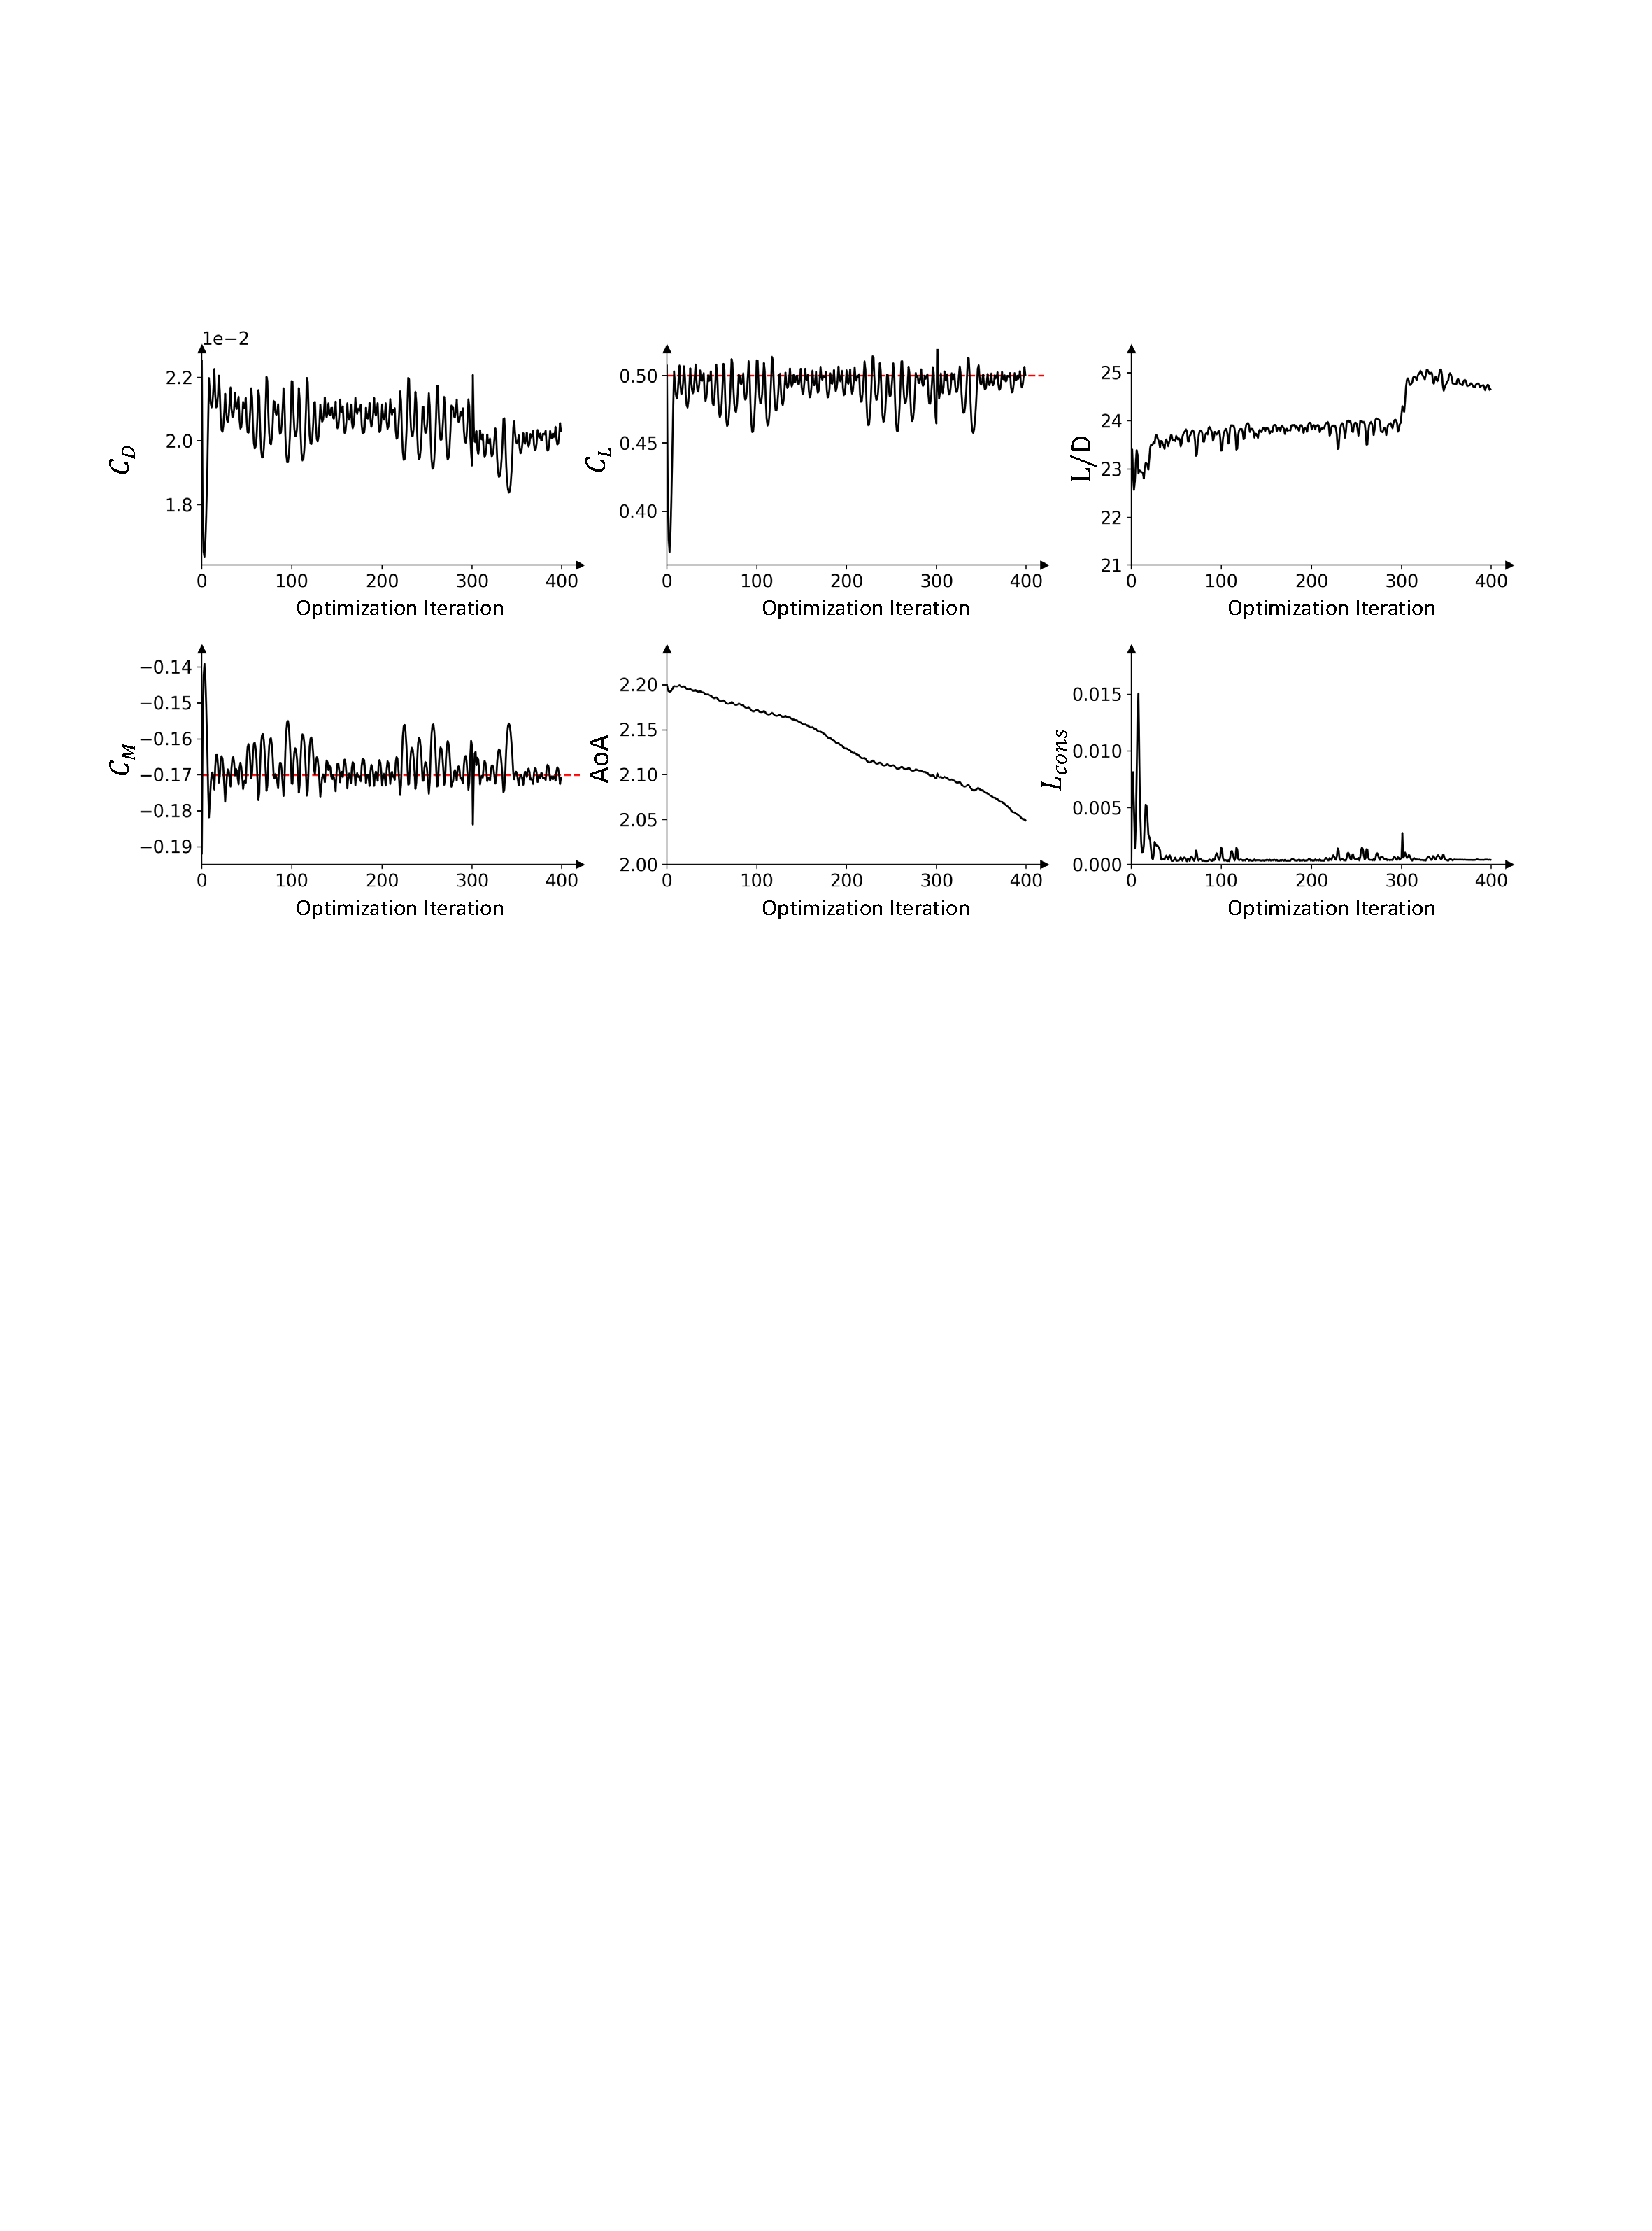
\includegraphics[width=1\linewidth]{chapter5/fig/crm_optim_history.pdf}
    \end{center}
    \caption{
        \small The optimization history of Case Study II. The dashed line in $C_L$ and $C_M$ figures demonstrates the optimization objectives.
    }
    \label{ch5:fig:cs2_history}
\end{figure}

\begin{figure}[!t]
    \begin{center}
        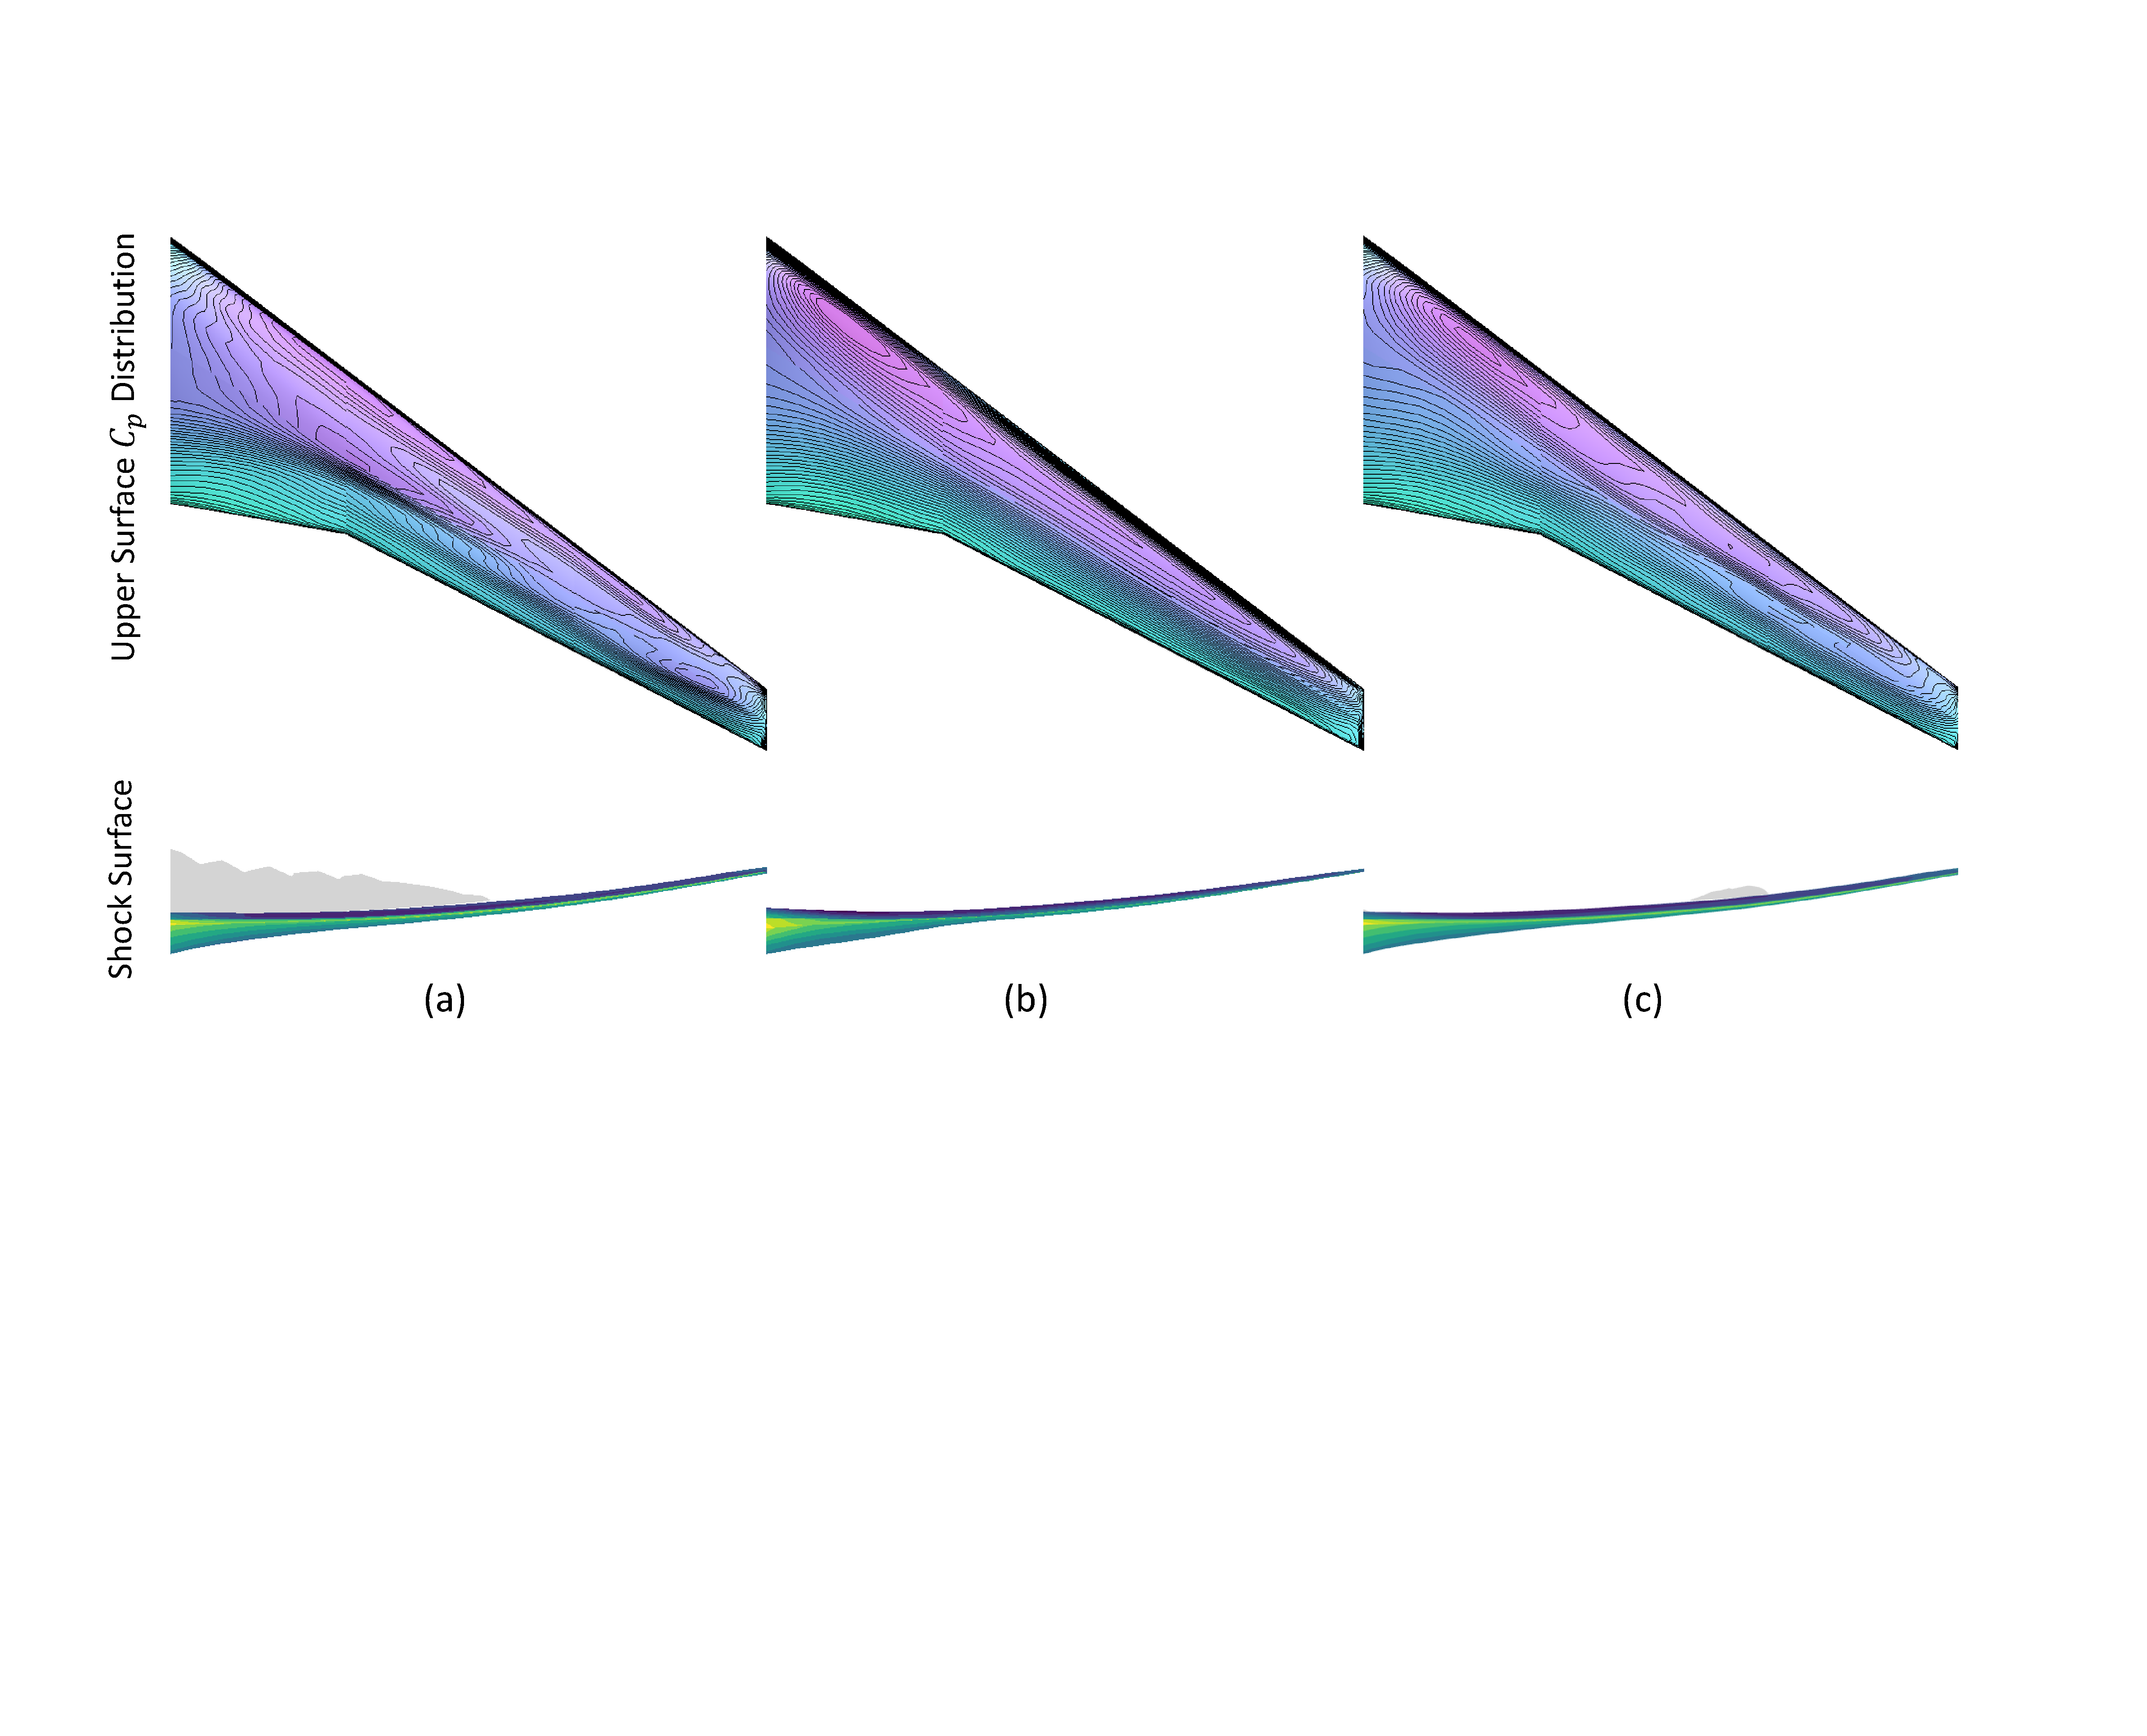
\includegraphics[width=1\linewidth]{chapter5/fig/crm_optim_cp.pdf}
    \end{center}
    \caption{
        \small A comparison of Case Study II on the pressure coefficient distributions and shock shapes of (a) the initial CRM wing, (b) the wing optimized with 192-point FFD, and (c) the wing optimized with DeepGeo.
    }
    \label{ch5:fig:cs2_cp}
\end{figure}

\begin{figure}[!h]
    \begin{center}
        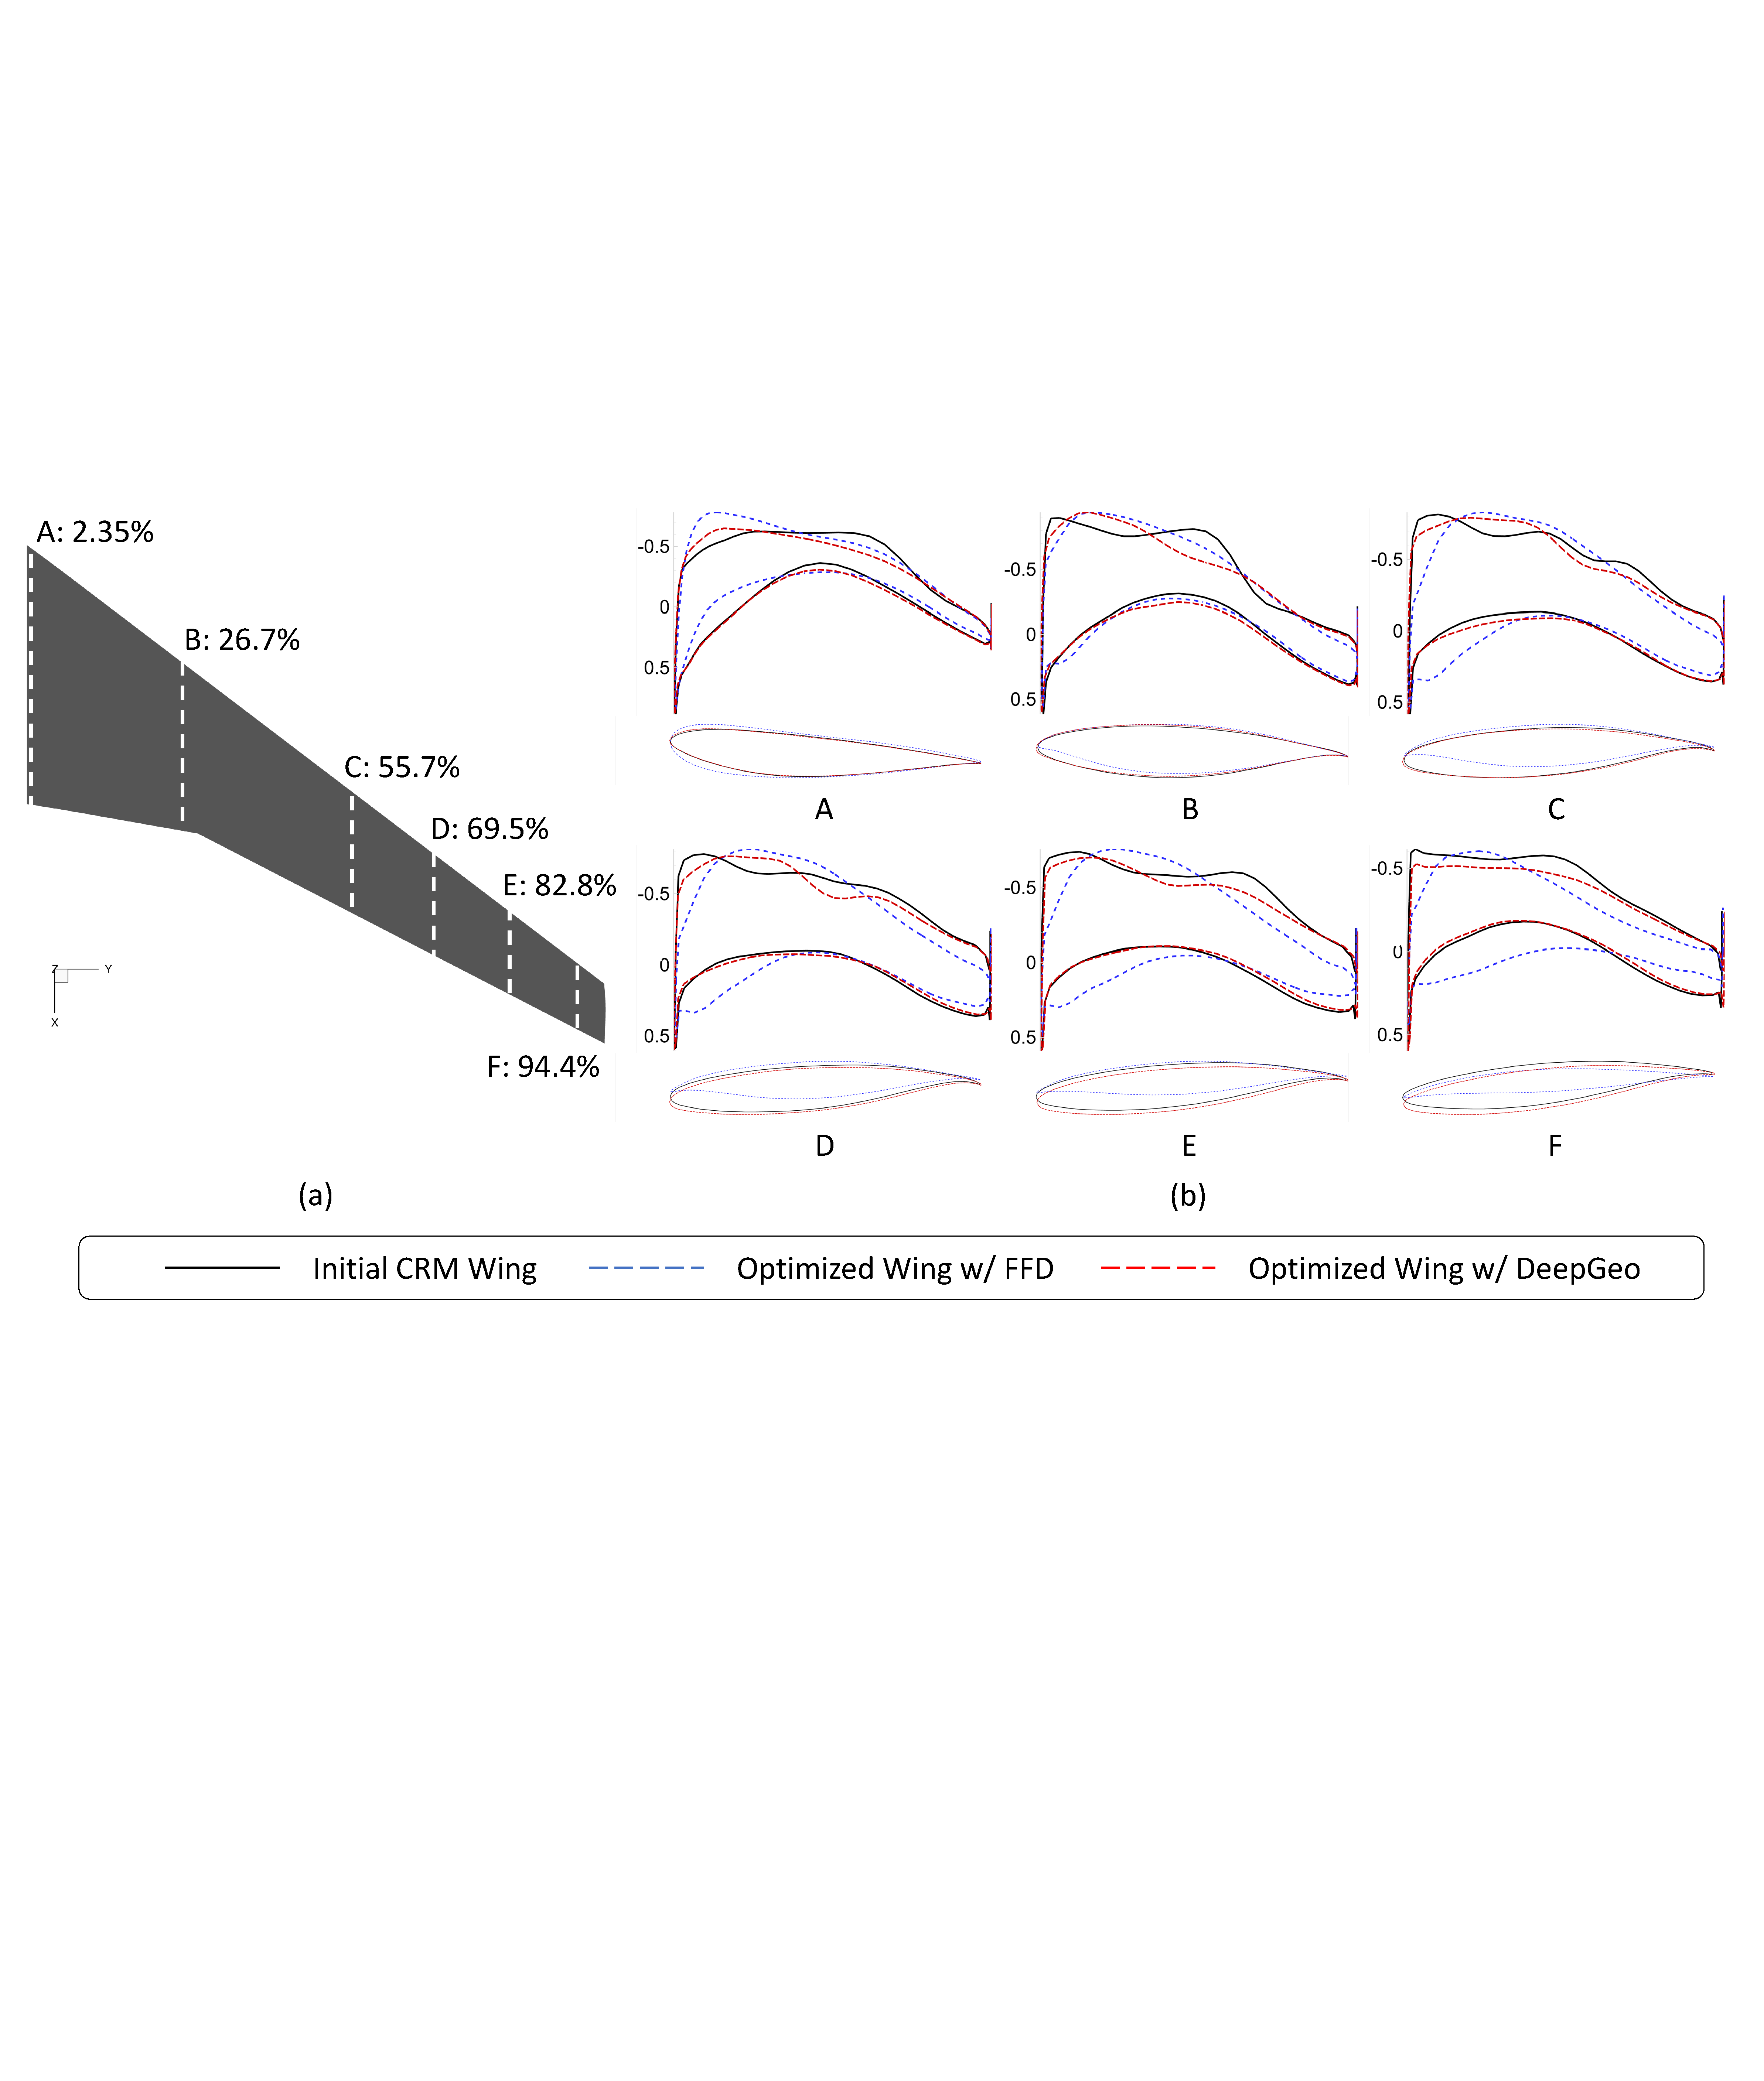
\includegraphics[width=1\linewidth]{chapter5/fig/crm_optim_slice.pdf}
    \end{center}
    \caption{
        \small A comparison of Case Study II on sliced geometries, including (a) the positions of slices, and (b) the shape variation and pressure coefficient distribution of each slice.
    }
    \label{ch5:fig:cs2_slice}
\end{figure}

Comparative quantitative results are presented in Tab.\ref{ch5:tab:crm_result}. The FFD results were obtained after extensive tuning, while DeepGeo achieved its results without requiring any parameter adjustments. 
The difference in the optimized drag coefficient $C_D$ is less than $0.5\%$. As noted by \citet{aa.Lyu2015}, even slight variations in FFD configuration can lead to increases of up to $2.4$ counts in the optimized drag coefficient.
Fig.~\ref{ch5:fig:cs2_history} shows the optimization history. The comparison with the history of the FFD-based optimization is provided in Appendix~\ref{ch5:sec:appendix_optim_history}.

Initially, DeepGeo parameterizes the CRM wing through self-initialization, similar to the approach used in the first case study on the 2D circle optimization. During the first 300 optimization iterations, the wing's lift-to-drag ratio ($L/D$) increases from $22.5$ to $23.8$.
Once the optimization converges, the partially optimized wing is reparameterized by self-initializing a new DeepGeo model.
The optimization continues after that.
The $L/D$ ratio reaches a maximum of $25.0$ before gradually decreasing, with the optimal result observed at the $320\text{th}$ iteration. The drag coefficient $C_D$ has been reduced by $10.9\%$.

In Fig.~\ref{ch5:fig:cs2_cp}, we compare the pressure distributions and shock wave patterns for both parameterization approaches. 
The shock waves are substantially reduced in both optimized results. The parallel alignment of pressure contour lines in both cases indicates improved aerodynamic performance, though they exhibit evident differences.
Fig.~\ref{ch5:fig:cs2_slice} compares 2D slices of the optimized wings at various locations along the wingspan. In terms of the constraint preservation, all six sectional slices across the span of DeepGeo's optimization result satisfy the $25\%$ original thickness constraint. FFD and DeepGeo yield distinct shapes: FFD results display very sharp leading edges and significant thickness variations along the span, while DeepGeo’s results show smaller deviations from the initial shape. The leading edges are less sharp, the trailing edges better adhere to geometric constraints, and the wing tips remain sufficiently thick so avoid extreme thinning.

The final design obtained with DeepGeo lies in a narrow design space close to the baseline geometry, which may be due to local convergence within the high-dimensional gradient-based optimization process under restrictive geometric constraints. 
The optimized shape tends to generate relatively smaller modifications of the initial design.
%However, this phenomenon is preferable for industry applications, as it preserves off-design performance with only minor modifications from the initial design, facilitating robust performance under different operating conditions. 
In contrast, the FFD-based optimization aggressively reduces the leading edge thickness to minimize on-design drag, potentially compromising low-speed aerodynamic performance~\cite{aa.Li2019} critical for landing and takeoff. Thus, DeepGeo’s approach is beneficial when starting from a good conceptual design, yielding a more controlled ASO pipeline with minimal adjustments.

In summary, DeepGeo achieves comparable aerodynamic performance to the best manually tuned FFD-based method with a simpler, less labor-intensive setup. Its ability to reduce the need for extensive tuning makes it an effective and practical choice for industrial aerodynamic optimization.
\subsection{Optimizing the Blended-Wing-Body Aircraft}
\label{ch5:sec:cs3}

We now demonstrate DeepGeo's capability to handle complex 3D geometries without tuning. To this end, we focus on optimizing the first-generation Boeing Blended-Wing-Body (BWB) design as shown in Fig.~\ref{ch5:fig:cs3_template_mesh}. The BWB aircraft configuration integrates the wing and fuselage into a single, seamless structure to enhance aerodynamic efficiency, reduce drag, and lower fuel consumption. The BWB used in this case study has a span of 280 feet, a total length of 144 feet and is designed to carry 800 passengers~\cite{aa.Liebeck2004}.
A notable challenge in this design is that the supersonic airflow creates significant shock waves, introducing strong drag forces. The key to optimization is refining the BWB shape to mitigate these drag-inducing effects.

\begin{table}[!b]
  \centering
  \caption{\small Aerodynamic shape optimization task specifications for the Case Study III.}
  \resizebox{1\columnwidth}{!} {
        \begin{tabular}{lllrr}
        \hline
        \multicolumn{1}{l}{\textbf{Objectives}} & \textbf{Functions/Variables} & \textbf{Description} & \multicolumn{1}{l}{\textbf{DeepGeo Quantity}} & \multicolumn{1}{l}{\textbf{FFD Quantity}} \\
        \hline
        \multicolumn{1}{l}{\textbf{Minimize}} & $C_D$  & Drag coefficient &        &  \\
        \hline
        \multicolumn{1}{l}{\multirow{3}[2]{*}{\textbf{With respect to}}} & $\Theta$ & Weights of DeepGeo & \num{151585} &         \\
        \multicolumn{1}{l}{} & $P_z$  & Control points' $z$ coordinates &        & 240 \\
        \multicolumn{1}{l}{} & $\alpha$ & Angle of attack & 1      & 1 \\
        \hline
        \multicolumn{3}{l}{\textbf{Total design variables}} & \num{151586} & 241 \\
        \hline
        \multicolumn{1}{l}{\multirow{5}[2]{*}{\textbf{Subject to}}} & $C_L=0.20056$ & Lift coefficient constraint & 1      & 1 \\
        \multicolumn{1}{r}{} & $C_M=0$ & Moment coefficient constraint & 1      & 1 \\
        \multicolumn{1}{r}{} & $t \ge 0.01 \; t_\text{original}$ & Minimum thickness constraints &        & 750 \\
        \multicolumn{1}{r}{} & $Vol \ge {Vol}_\text{original}$ & Minimum volume constraint & 1      &  1 \\
        \multicolumn{1}{r}{} & $0 \leq \alpha \leq 2.5$ & Angle of attack constraint & 1      &  1 \\
        \hline
        \multicolumn{3}{l}{\textbf{Total constraints}} & 7      & 754 \\
        \hline
        \multicolumn{3}{l}{\textbf{Need value range limits for each DV?}} & NO     & YES \\
        \hline
        \end{tabular}%
    }
  \label{ch5:tab:bwb_DV_cons}%
\end{table}%

\subsubsection{Problem Formulation}

The optimization objective is to minimize the drag coefficient $C_D$ while constraining the lift coefficient $C_L$ to $0.20056$ and ensuring a pitching moment coefficient $C_M$ of 0. This single-point optimization problem is performed under fully turbulent flow conditions at a Mach number of $0.85$, Reynolds number of $5\times10^6$ and an initial angle of attack of $0.58^{\circ}$. The optimization is performed on both the mesh that has $1,070,080$ cells, corresponding to the same setting as the L2 grid configuration in~\citet{aa.Lyu2014}. Shape modifications are allowed only along the $z$ axis to maintain a constant projected area, and the aircraft volume is constrained to remain above its initial value, preventing shrinkage that could reduce drag but compromise capacity. Compared to the optimization task of the CRM wing, the task for BWB aircraft is less constrained. Tab.~\ref{ch5:tab:bwb_DV_cons} summarizes the experimental setup. 

\begin{figure}[ht]
    \begin{center}
        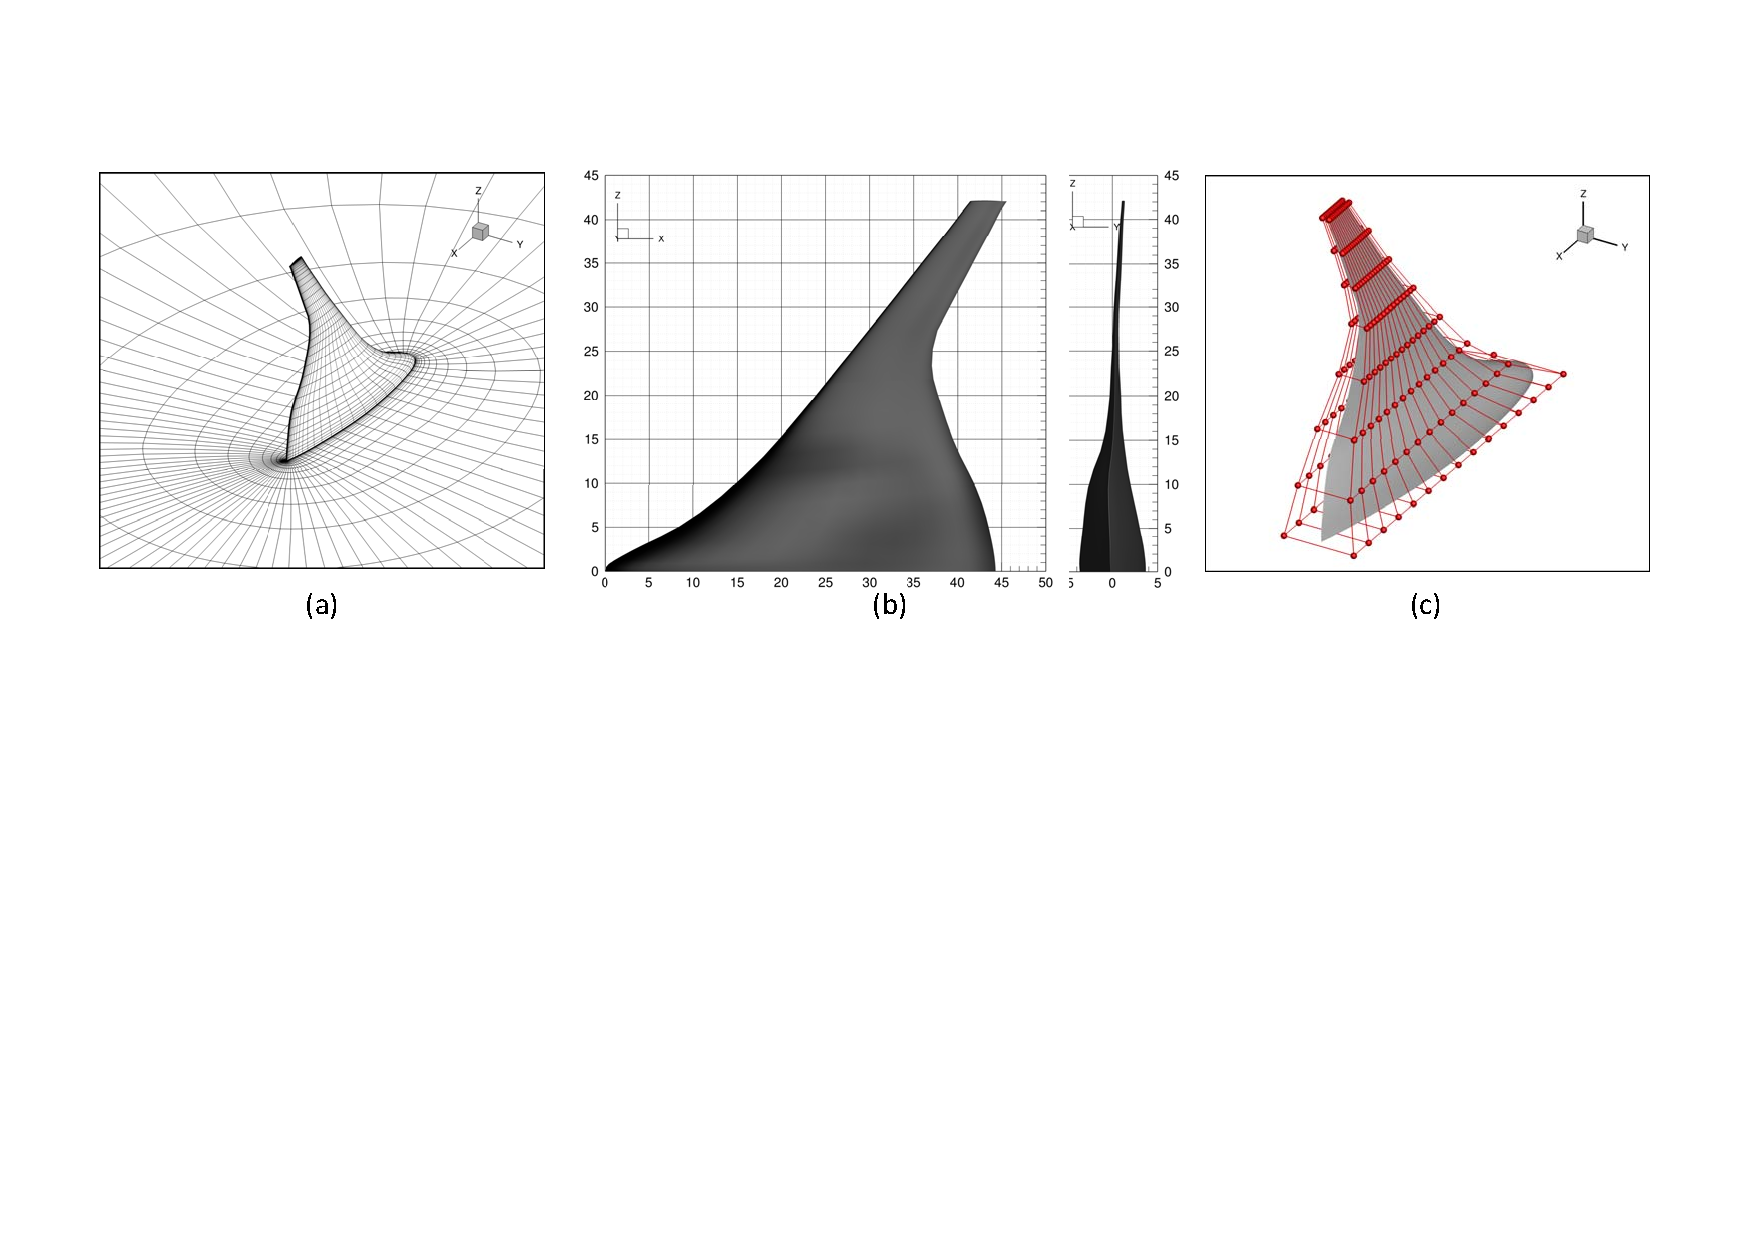
\includegraphics[width=1\linewidth]{chapter5/fig/bwb_template_mesh_initial_geometry.pdf}
    \end{center}
    \caption{
        \small Geometric setup for the BWB Case Study. (a) DeepGeo template mesh. (b) the initial BWB aircraft geometry and (c) the 240-point FFD setting.
    }
    \label{ch5:fig:cs3_template_mesh}
\end{figure}

\begin{figure}[htb]
    \begin{center}
        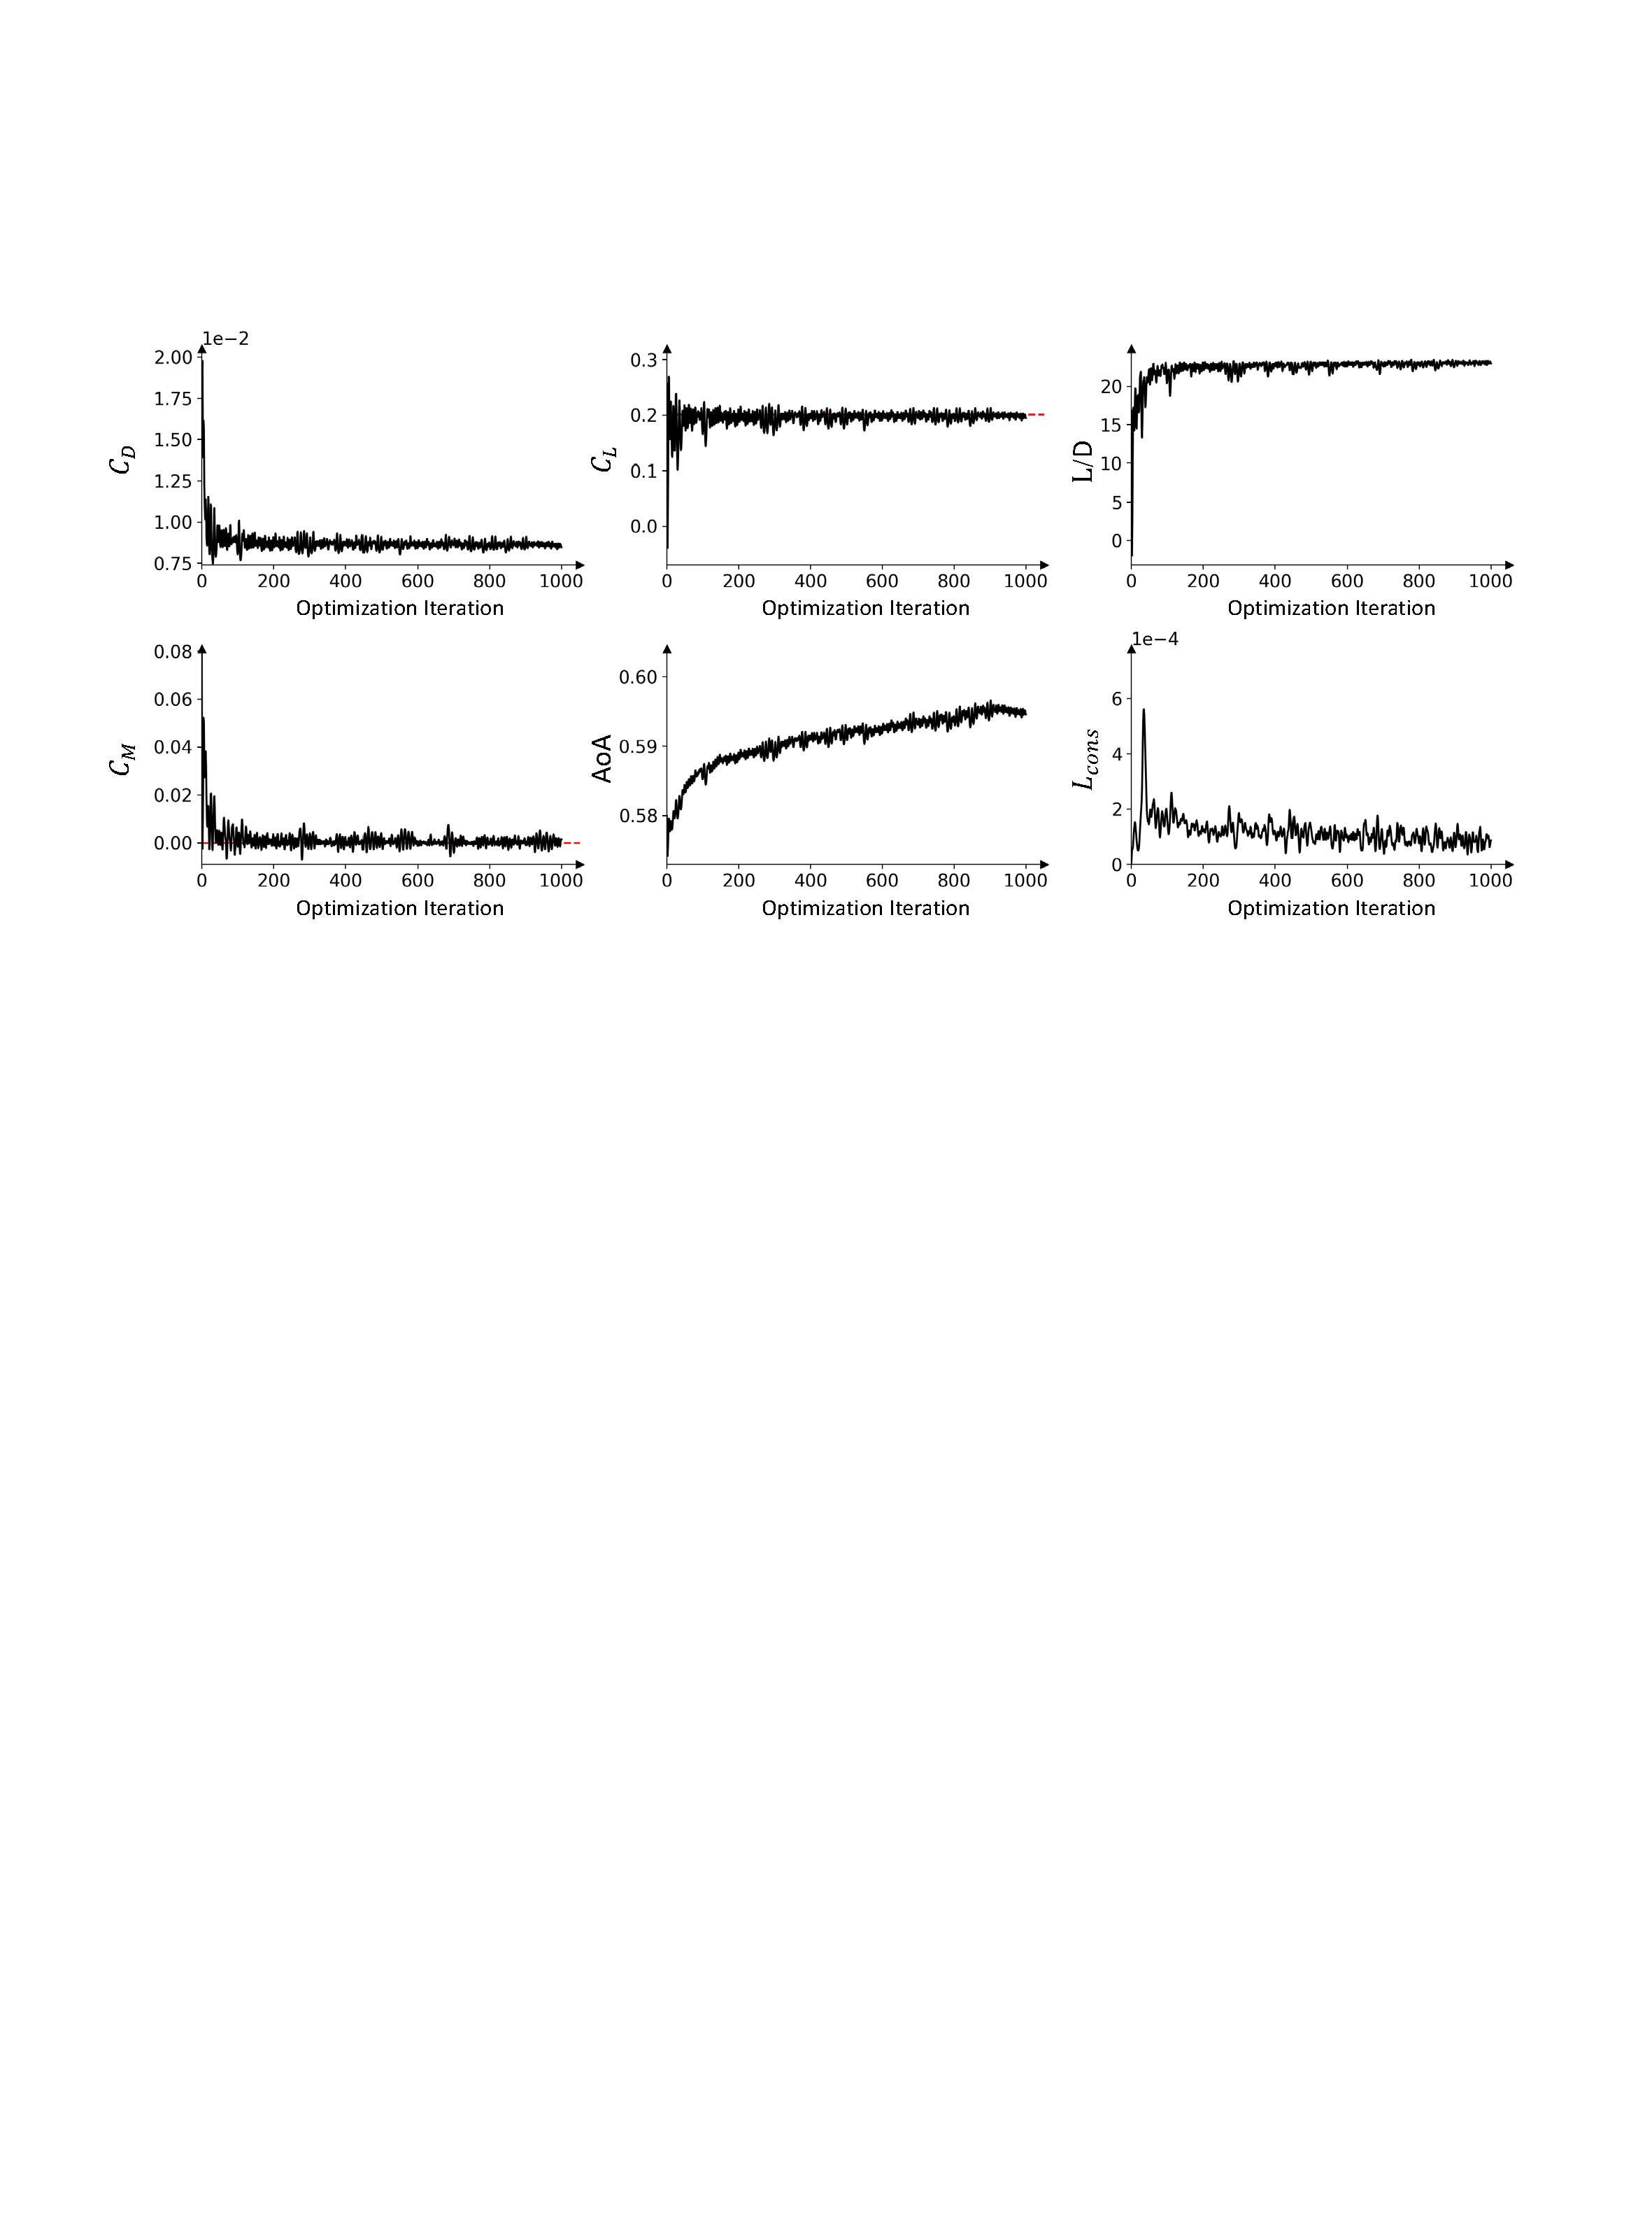
\includegraphics[width=1\linewidth]{chapter5/fig/bwb_L2_optim_history.pdf}
    \end{center}
    \vspace{-7mm}
    \caption{
        \small Evolution of important quantities during optimization for the BWB case. The dashed line in the $C_L$ and $C_M$ plots represent the optimization objectives.
    }
    \label{ch5:fig:cs3_history}
\end{figure}

\subsubsection{Configuring DeepGeo}

DeepGeo uses the L2 grid as template mesh. Similarly, DeepGeo parameterizes the BWB aircraft geometry through self-initialization, learning to generate all-zero deformation. 
Shape variations generated by DeepGeo are limited to the $z$ axis, in line with the allowed modifications specified by the optimization problem. This avoids the need for additional geometric constraints on the leading edge (LE) and trailing edge (TE).
The aerodynamic objective function $\cO_{CFD}$ and the volume constraint $\cL_{cons}$ from Eq.~\ref{ch5:eq:asoObj} are defined as
%
\begin{align}
 \cO_{CFD} &= \left| C_D \right| + \left| C_L-0.5 \right| + \left| C_M \right| \; , \\
 \cL_{cons} & = {\max \left(Vol(V^S)-{Vol}_\text{original}(S), 0\right)} ^2 \; .
\end{align}
%

\begin{figure}[!t]
    \begin{center}
        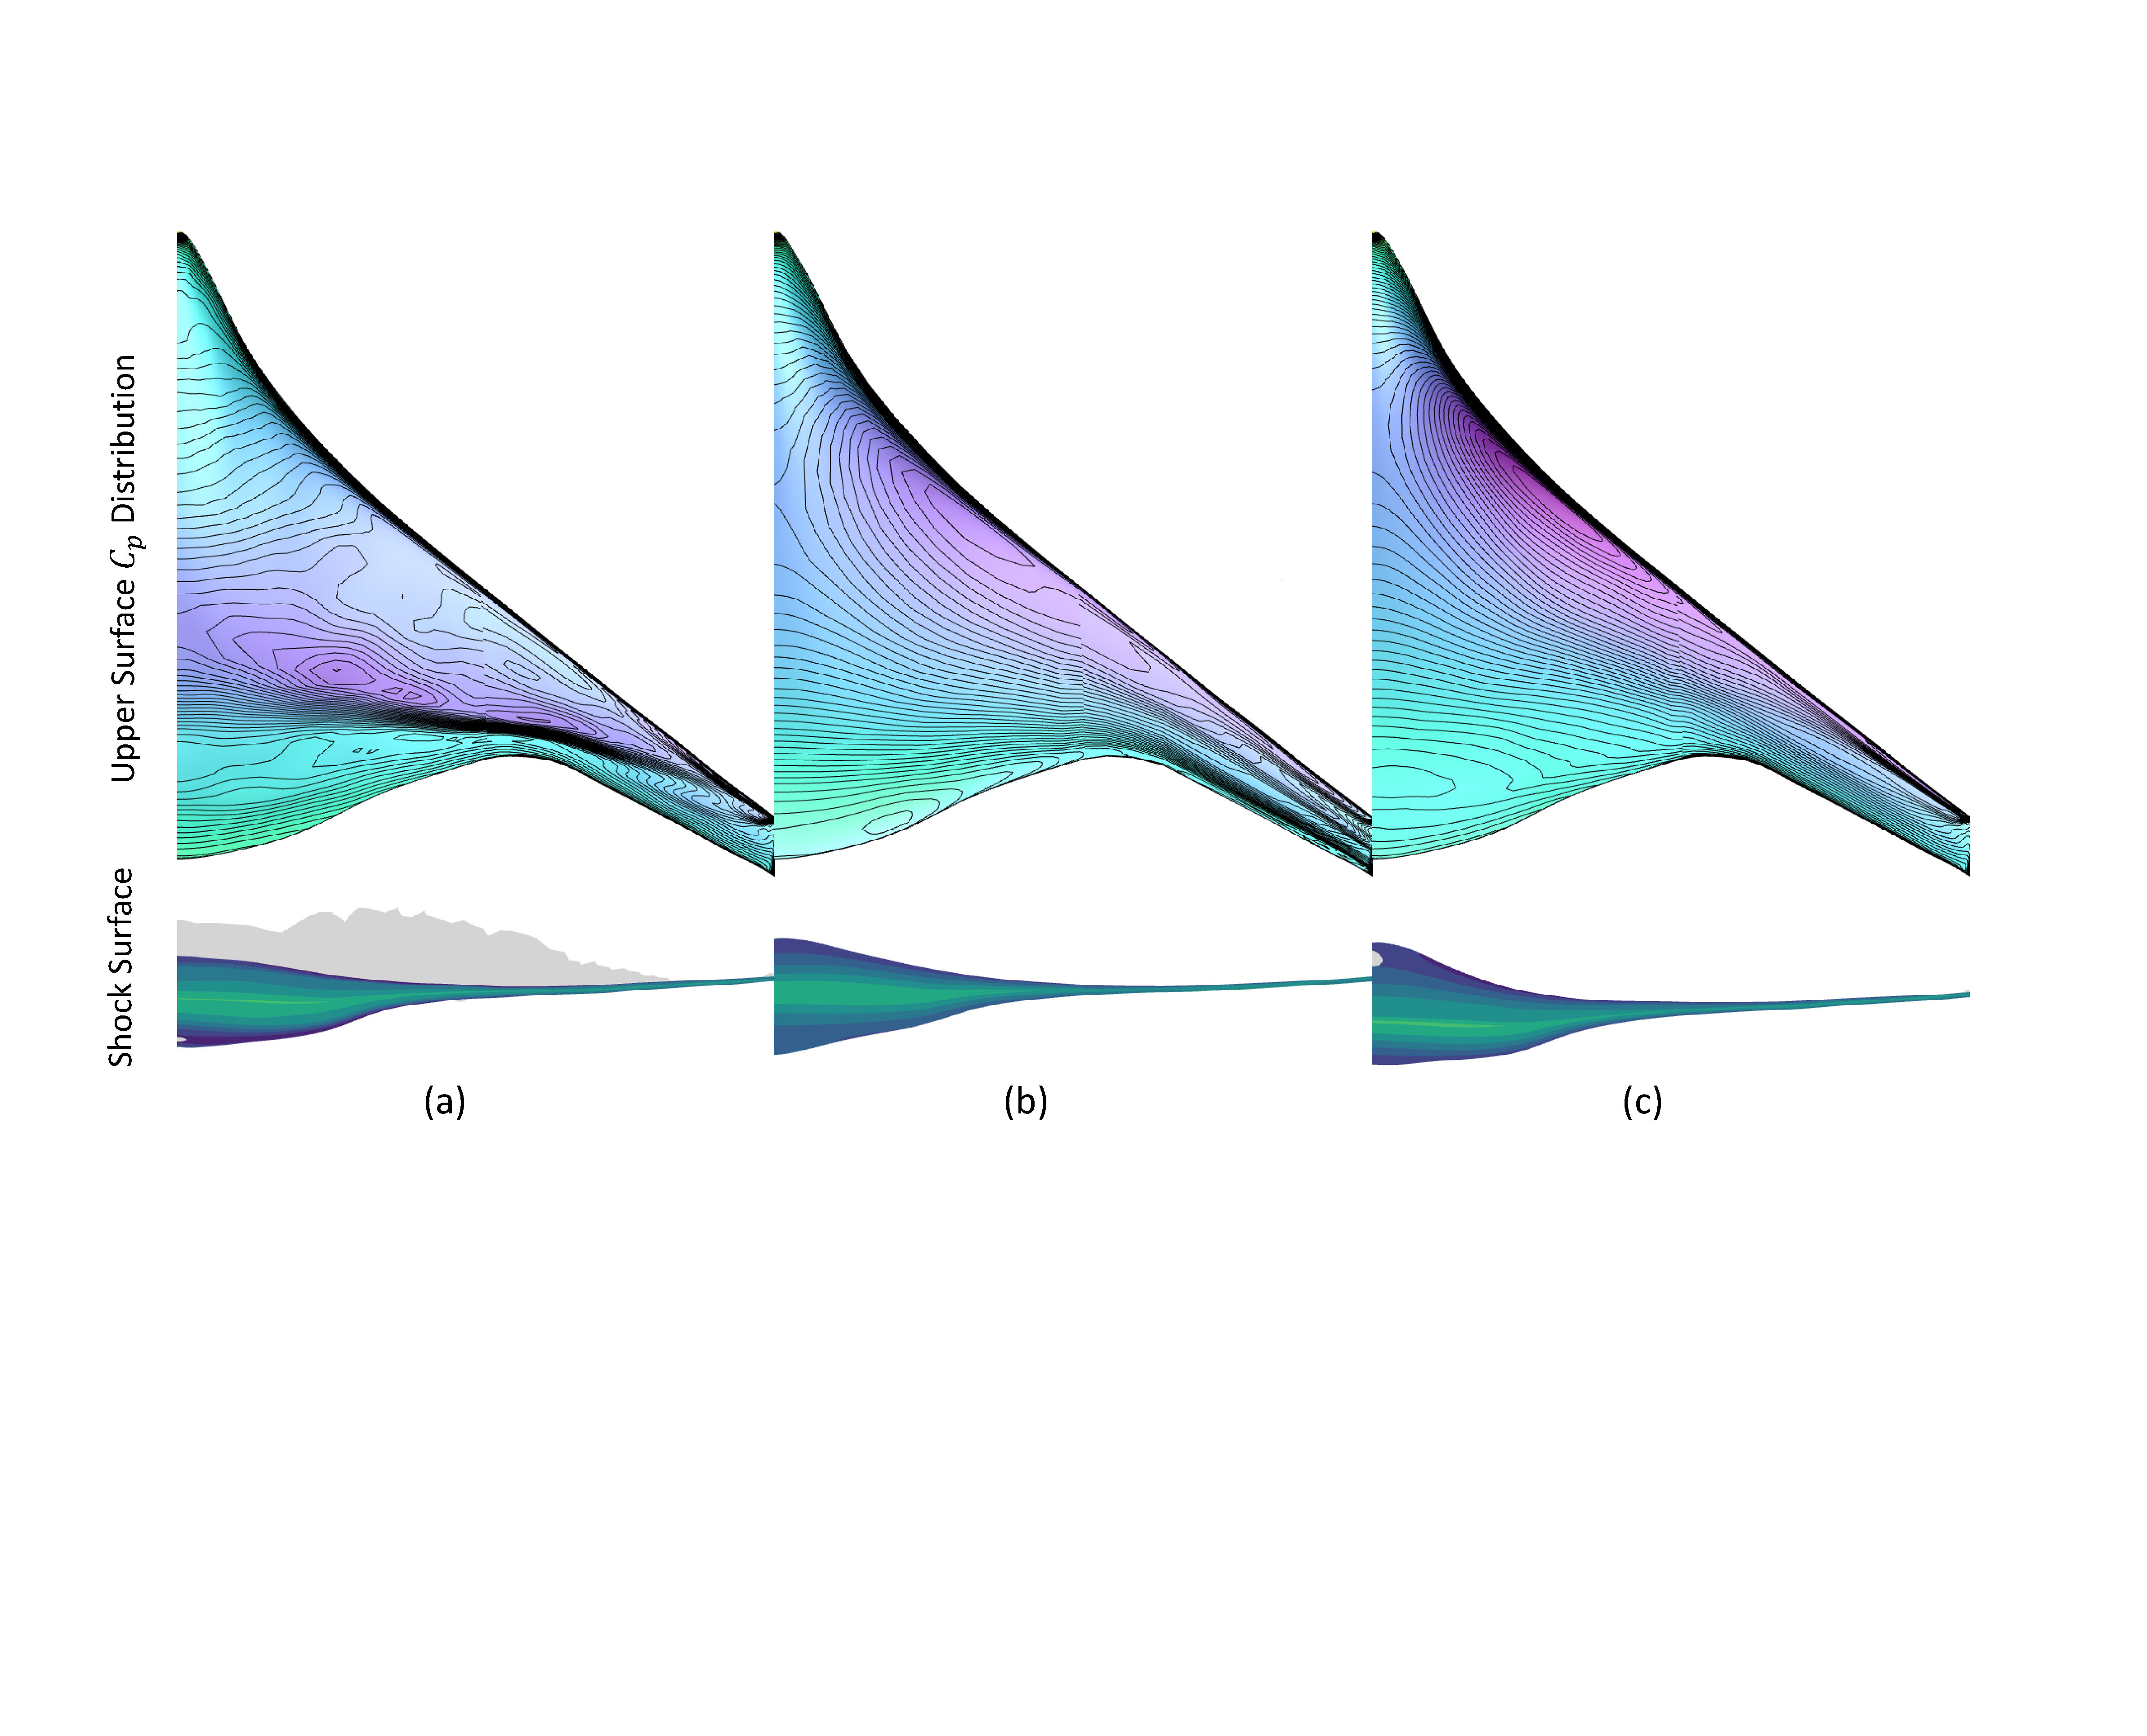
\includegraphics[width=1\linewidth]{chapter5/fig/bwb_optim_cp.pdf}
    \end{center}
    \caption{
        \small A comparison of Case Study III on the pressure coefficient distributions and shock shapes of (a) the initial CRM wing, (b) the wing optimized with 240-point FFD, and (c) the wing optimized with DeepGeo.
    }
    \label{ch5:fig:cs3_cp}
\end{figure}

\begin{figure}[!th]
    \vspace{2mm}
    \begin{center}
        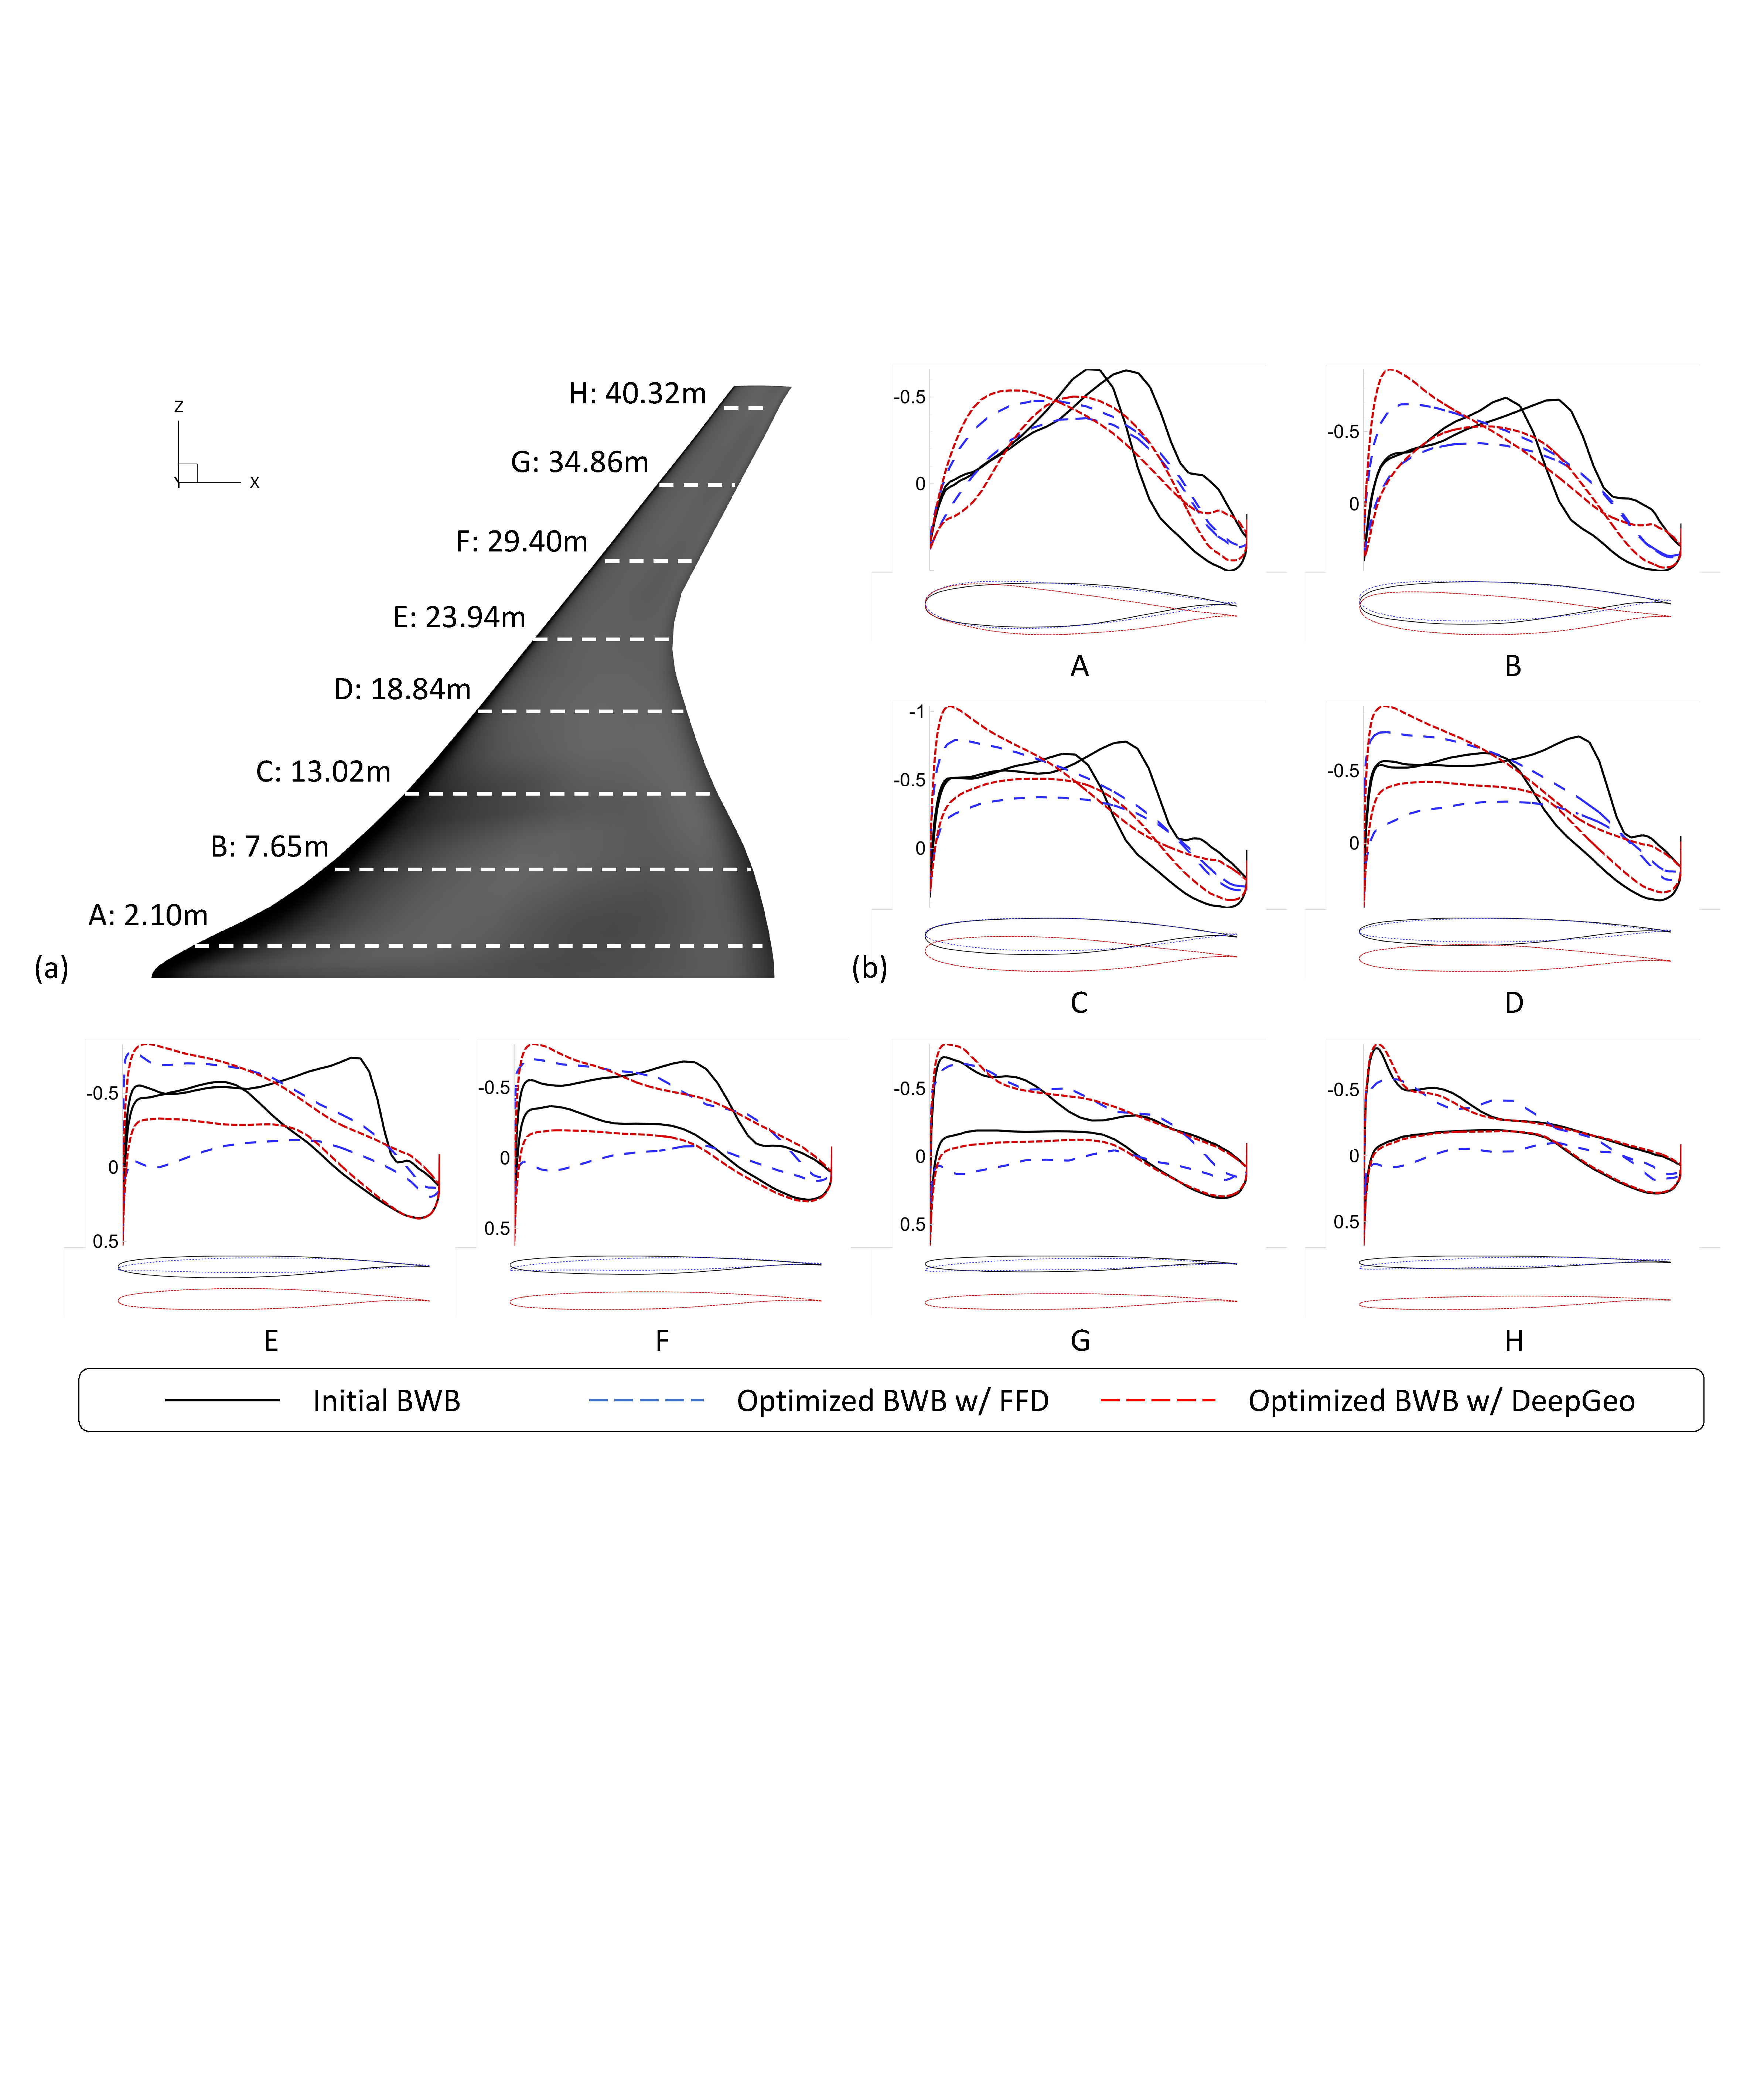
\includegraphics[width=1\linewidth]{chapter5/fig/bwb_optim_slice.pdf}
    \end{center}
    \caption{
        \small A comparison of Case Study III on sliced geometries, including (a) the positions of slices, and (b) the shape variation and pressure coefficient distribution of each slice.
    }
    \label{ch5:fig:cs3_slice}
\end{figure}

% \begin{table}[htbp]
%   \centering
%   \caption{BWB aircraft optimization results of the Case Study III.}
%     \begin{tabular}{l|ccccc}
%     \hline
%     \textbf{Parameterization} &  \multicolumn{1}{l}{\textbf{Final} $C_D$ {\footnotesize(counts)}} & \multicolumn{1}{l}{\textbf{Final} $C_L$} & \multicolumn{1}{l}{\textbf{Final} $C_M$} & \multicolumn{1}{l}{\textbf{Final} $\alpha$} & \multicolumn{1}{l}{\textbf{Final} {\footnotesize $Vol/Vol_\text{original}$}}\\
%     \hline
%     \multicolumn{6}{l}{\textbf{w/ L3 Grid}} \\
%     \hline
%     \textbf{DMM} & \num{104.14}  & \num{0.20055}  & \num{3.7524e-3}  & 0.60 & 99.1\%\\
%     \textbf{FFD} & \num{103.33}  & \num{0.20056}  & \num{-1.1998e-6} & 2.29 & \\
%     \hline
%     \multicolumn{6}{l}{\textbf{w/ L2 Grid}} \\
%     \hline
%     \textbf{DMM} & \num{86.42}  & \num{0.20072}  & \num{9.8807e-4} & 0.60 & 99.6\%\\
%     \textbf{FFD} &   &   &   &  & \\
%     \hline
%     \end{tabular}%
%   \label{tab:bwb_result}%
% \end{table}%

\begin{table}[!t]
  \centering
  \caption{\small BWB aircraft optimization results of the Case Study III.}
    \begin{tabular}{lcccc}
    \hline
    \textbf{Parameterization} &  \multicolumn{1}{l}{\textbf{Final} $C_D$ {\footnotesize(counts)}} & \multicolumn{1}{l}{\textbf{Final} $C_L$} & \multicolumn{1}{l}{\textbf{Final} $C_M$} & \multicolumn{1}{l}{\textbf{Final} $\alpha$}\\
    \hline
    \textbf{DeepGeo} & \num{86.42}  & \num{0.20072}  & \num{9.8807e-4} & 0.60 \\
    \textbf{FFD} & \num{87.05}  & \num{0.20056}  & \num{2.4675e-9}  & 2.47 \\
    \hline
    \end{tabular}%
  \label{ch5:tab:bwb_result}%
\end{table}%

\subsubsection{Configuring the Free-Form Deformation Baseline}

The FFD configuration follows the well-established settings proposed by~\citet{aa.Lyu2014}. This configuration uses 240 control points, as shown in Fig.~\ref{ch5:fig:cs3_template_mesh}(c). A minimal thickness constraint is added to prevent crashes caused by the negative volume error during optimization. The FFD baseline case uses IPOPT implemented in pyOptSparse~\cite{aa.Wu2020} for optimization.

\subsubsection{Results and Analysis}

Fig.~\ref{ch5:fig:cs3_history} shows the evolution of key aerodynamic quantities throughout the optimization process. The comparison with the FFD-based optimization history is provided in Appendix~\ref{ch5:sec:appendix_optim_history}. The optimization constraints on $C_L$ and $C_M$ are quickly fulfilled. The DeepGeo-based optimization achieves a shock-free design by the 149th iteration, and the number of total iterations remains within the same order of magnitude as the FFD-based optimization. Quantitative results comparing the automatic DeepGeo with the best manually configured FFD baseline are presented in Tab.~\ref{ch5:tab:bwb_result}. In terms of aerodynamic performance, DeepGeo achieves $47.8\%$ drag reduction in total and the drag performance is $0.63$ counts lower than FFD's result in $C_D$. Furthermore, as can be seen in Fig.~\ref{ch5:fig:cs3_cp}, the optimized FFD configuration exhibits a double shock near the wing tip, which is an undesirable feature in practical applications. In contrast, the DeepGeo-optimized design is shock-wave-free near the tip. 

Fig.~\ref{ch5:fig:cs3_slice}, provides a sectional analysis of geometry variations along the wingspan. The DeepGeo-optimized result shows more drastic changes in the spanwise bending and is less tilted upwards, while the shape variation on each slice is less significant. Similar to the results for the CRM wing, the FFD-optimized design has much sharper leading edges, which may negatively impact low-speed aerodynamic performance.

In summary, DeepGeo provides greater deformation freedom and, consequently, a broader design space for exploration when given less restrictive geometric constraints. In contrast, achieving similar flexibility with FFD requires users to manually implement various global design functions and introduce additional design variables, such as sweep, twist and dihedral functions, while carefully constraining each new design variable to avoid optimization failures. This approach requires significant additional engineering effort, making DeepGeo a more efficient and flexible alternative.
\section{Discussion}

\subsection{Justification of DeepGeo's Over-Parameterization and Complexity}
\label{ch5:sec:complexity}

Traditional parameterizations rely on low-dimensional design variables and suffer from several key limitations:
\begin{itemize}
    \item They require extensive manual intervention. This includes selecting an appropriate method, configuring parameters to balance flexibility, smoothness and robustness, and carefully defining parameter constraints. Moreover, capturing essential inter-parameter correlations--such as the twisting or sweeping global functions used in wing optimization--must be explicitly hard-coded, which heavily depends on domain expertise.

    \item They rely on costly trial-and-error procedures. The quality of results often depends on iterative manual experimentation. For example, an inappropriate FFD configuration of a CRM wing can lead to a 42\% reduction in drag improvement~\cite{aa.Lyu2015}, making multiple optimization attempts necessary to achieve a near-optimal design.
\end{itemize}

In contrast, DeepGeo leverages over-parameterization to enable its capability, adaptability and robustness. The large number of parameters is not a drawback but a necessary design choice that allows DeepGeo to capture complex geometric variations and to implement the benefits described above through a fully automatic, data-independent process. During its initialization phase, as defined by Eq.~\ref{ch5:eq:weightInit}, DeepGeo automatically learns a design parameterization by combining the selection, setting and integration of parameters into an adaptive framework. Consequently, DeepGeo’s most significant advantages over traditional parameterizations are the reduction in manual intervention, minimized dependency on expert prior and the elimination of costly trial-and-error practices.

% !TEX root = ../main.tex
% !TEX spellcheck = en-US

\begin{figure}[tbh]
    \begin{center}
        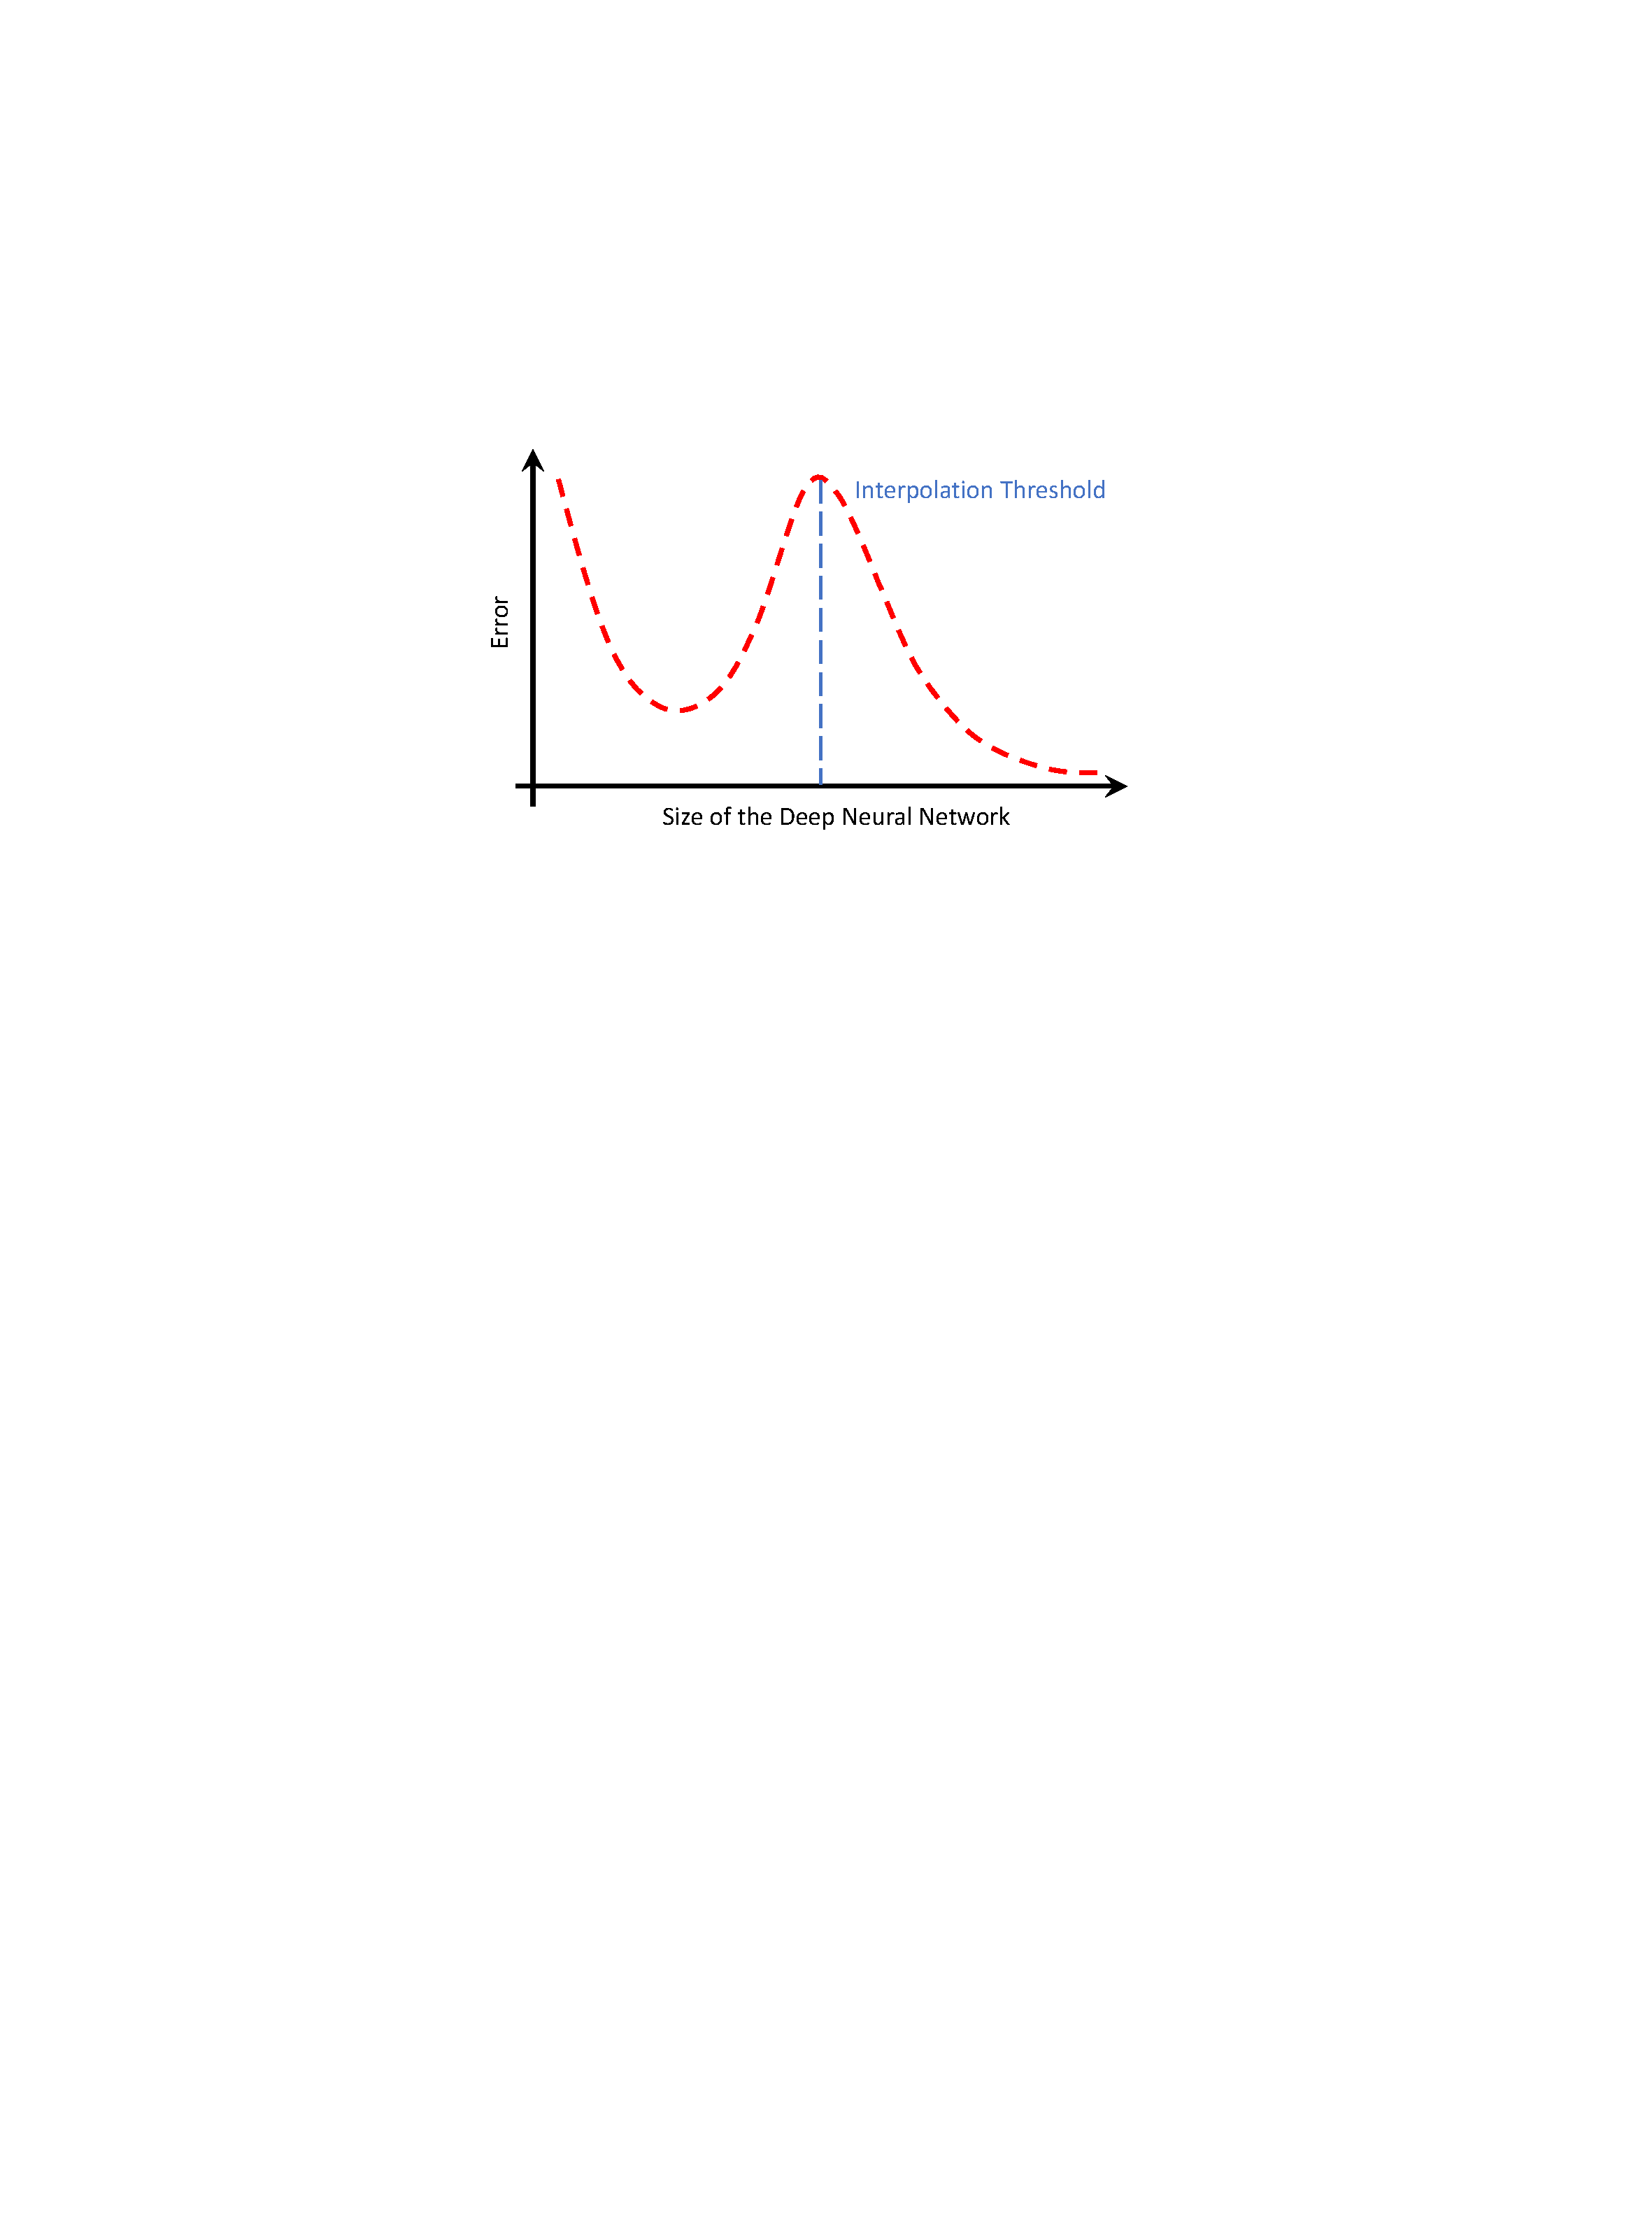
\includegraphics[width=1\linewidth]{chapter5/fig/double_descent.pdf}
    \end{center}
    \vspace{-5mm}
    \caption{
        \small  The \textit{double descent} phenomenon in deep learning models.
    }
    \label{ch5:fig:double_descent}
\end{figure}

Using the number of weights for as a proxy for  DeepGeo's actual complexity is misleading when comparing it to methods that do not rely on deep learning. This is because in DeepGeo, as in most deep-learning approaches with high-dimensional parameter spaces,
the large parameter count does not necessarily translate into excessive complexity. Recent studies have revealed the \textit{double descent} phenomenon~\cite{ai.Belkin2019,ai.Spigler2019}, as illustrated in Fig.~\ref{ch5:fig:double_descent}, which shows that as model size increases, the generalization error first decreases, then rises near the interpolation threshold, and finally decreases again with further over-parameterization. This second descent implies that highly over-parameterized models can be more effective despite their excessive parameter amount. This behavior is due to the weight correlations developed in neural networks~\cite{ai.Jin2020b} and the reduced number of independent degrees of freedom during training. Therefore, a more meaningful indicator of DeepGeo's complexity is its \textit{effective dimensionality}, which quantifies the number of independent directions in parameter space that influence the model’s behavior--akin to reduced dimensions in model order reduction. A well-trained network typically exhibits low \textit{effective dimensionality}, meaning that its function lies in a relatively low-dimensional parameter subspace despite its large number of parameters, and it can effectively compress the information from data.
\begin{table}[htbp]
  \centering
  \caption{Comparison of effective dimensionality for DeepGeo models. The values of random model are based on 20 repeats.}
  \resizebox{\textwidth}{!}{  
    \begin{tabular}{llllll}
    \hline
    \multirow{2}[2]{*}{\textbf{Model}} & \textbf{Layer 1} & \textbf{Layer 2} & \textbf{Layer 3} & \textbf{Output Layer} & \multirow{2}[2]{*}{\textbf{Overall}}\\
           & weight ratio: $0.1\%$ & weight ratio: 11.0\% & weight ratio: 87.9\% & weight ratio: 1.0\% &  \\
    \hline
    Random & $264.0\pm44.9$ & $114.4\pm63.1$ & $226.5\pm33.5$ & $332.7\pm34.4$ & $215.3\pm37.1$ \\
    \hline
    2D Circle & $2.6$  & $2.9$  & $2.6$  & $3.9$  & $2.6$ \\
    \hline
    CRM Wing & $2.3$  & $0.4$  & $0.1$  & $4.8$  & $0.2$ \\
    \hline
    BWB Aircraft & $134.8$ & $51.5$ & $24.6$ & $-0.5$ & $27.4$ \\
    \hline
    \end{tabular}%
  }
  \label{ch5:tab:double_descent}%
\end{table}%

To empirically validate this, we compute DeepGeo’s \textit{effective dimensionality} using a metric based on the eigenvalues of the symmetric Hessian matrix of DeepGeo's weights~\cite{ai.Maddox2020} (as defined by Equation~\ref{ch5:eq:response_effective_dimensionality}). More details are included in Appendix~\ref{ch5:sec:appendix_effe_dim}. As shown in Table~\ref{ch5:tab:double_descent}, the initialized DeepGeo model has significantly lower effective dimensionalities compared to randomly initialized ones. This supports our claim that DeepGeo’s actual complexity is far less than its parameter count may suggest.

\subsection{Justification of DeepGeo's Smoothness, Expressiveness and Role of $L_{reg}$}

DeepGeo provides both global surface smoothness and sufficient deformation freedom to support high-fidelity design optimization. Several factors contribute to this. First, the smoothness arises naturally from the inherent properties of its MLP backbone, known in literature as the frequency principle~\cite{ai.Xu2019f,ai.Xu2020c} or spectral bias~\cite{ai.Rahaman2019}. As a result, the network tends to prioritize low-frequency features, while high-frequency components typically require more training iterations to emerge. Since ASO usually requires fewer iterations to converge than for  typical deep learning training, undesired high-frequency patterns, such as bumps or discontinuities, are unlikely to appear. Second, DeepGeo learns to create a shape deformation field rather than a full geometry from scratch and such a field is inherently smoother. For instance, when deforming an airfoil, DeepGeo does not need to reconstruct sharp trailing edges or rounded leading edges from zero. Instead, it learns a smooth transformation that modifies these features, simplifying the learning and contributing to overall surface regularity. Third, the use of a gradient-descent-based optimizer leads to smooth transitions in the design trajectory. At each iteration, the newly deformed geometry is a slight variant of the previous one. This mostly avoids abrupt or unstable geometric transformations.

DeepGeo’s expressiveness is supported by its over-parameterized MLP structure and, according to the universal approximation theory~\cite{ai.Barron1993,ai.Poggio2017}, this expressiveness is up-bounded by the model size. However, empirical results in Section~\ref{ch5:sec:complexity} show that the current model size has enabled the over-parameterization effect for all ASO tasks presented in this work. If DeepGeo were to be applied to significantly more complex tasks, increasing model size might be necessary.

The Hessian-based regularization loss $L_{reg}$, though introduced to stabilize volumetric mesh deformation, directly penalizes the magnitude of the network’s Hessian, and could potentially constrain DeepGeo's frequency behavior. While a full understanding of theoretical effects of this regularization on the model’s spectral properties would require further investigation, our empirical results do not indicate a significant loss in DeepGeo's expressiveness when $L_{reg}$ is properly weighted. As shown in Figure~\ref{ch5:fig:w_loss_reg_ablation}, even changing the weight of $L_{reg}$ by several orders of magnitude produces nearly identical deformed shapes. Furthermore, we analyze the gradient magnitudes of $\cO_{CFD}$ and $L_{reg}$ with respect to DeepGeo’s parameters at the start of design optimization. As shown in Table~\ref{ch5:tab:gradient_norm}, the norm of $\nabla L_{reg}$ is multiple orders of magnitude smaller than that of $\nabla \cO_{CFD}$ across all layers. This demonstrates that the physical objective driven by the adjoint solver is the dominant force that shapes DeepGeo's behavior.

\begin{table}[htbp]
  \centering
  \caption{The comparison of mean vector norms of $\nabla \cO_{CFD}$ and $\nabla L_{reg}$ with respect to all DeepGeo's layers}
    \begin{tabular}{lcccc}
    \hline
    \multirow{2}[4]{*}{ASO Case} & \multicolumn{4}{c}{Mean Vector Norm of $\nabla \cO_{CFD}$}\\
\cline{2-5}           & Layer 1 & Layer 2 & Layer 3 & Output Layer\\
    \hline
    2D Circle & 0.1825 & 0.4186 & 0.5105 & 6.3915\\
    CRM Wing & 0.1254 & 0.2814 & 0.2411 & 6.4747 \\
    BWB Aircraft & 0.1137 & 0.2166 & 0.1495 & 1.3316\\
    \hline
    \multirow{2}[4]{*}{ASO Case} & \multicolumn{4}{c}{Mean Vector Norm of $\nabla L_{reg}$}\\
\cline{2-5}           & Layer 1 & Layer 2 & Layer 3 & Output Layer\\
    \hline
    2D Circle & 0.0003 & 0.0003 & 0.0009 & 0.0235\\
    CRM Wing & 9.4266$\times 10^{-5}$ & 9.9453$\times 10^{-5}$ & 3.8320$\times 10^{-5}$ & 0.0016 \\
    BWB Aircraft & 0.0009 & 0.0008 & 0.0003 & 0.0034\\
    \hline
    \end{tabular}%
  \label{ch5:tab:gradient_norm}%
\end{table}%

Additionally, DeepGeo is different from traditional spectral parameterization methods used in ASO, such as \citet{aa.Li2019c,aa.Li2021c}. Those methods rely on explicit mode truncation for dimensionality reduction, which limits the design space in advance. In contrast, DeepGeo does not manually cut off its spectrum, it instead adapts its behavior according to different geometries and design tasks through its optimization.

Recent advances in computer vision and graphics have introduced techniques such as positional embeddings~\cite{ai.Vaswani2017} and feature grids~\cite{ai.Mueller2022} to inject high-frequency detail into MLPs. These techniques offer promising directions for future work aimed at implementing DeepGeo’s controllable smoothness and expanding the model's expressiveness when needed.

\section{Conclusion}
This research introduces a novel framework that leverages deep geometric learning to implement a fully automated shape parameterization method for Aerodynamic Shape Optimization (ASO).
By automating the parameterization process, DeepGeo significantly enhances efficiency and robustness over traditional methods, minimizing the need for manual intervention while maintaining optimization performance that is either superior or at least comparable to the best manually tuned techniques.
Specifically, in comparison to the state-of-the-art Free-Form Deformation (FFD) model, DeepGeo fully automates the handling of diverse geometries in both 2D and 3D. In contrast, FFD requires users to design a custom configuration for each task to achieve optimal performance, which demands extensive tuning and strong domain prior knowledge.

Additionally, DeepGeo integrates Computational Fluid Dynamics (CFD) mesh deformation directly into the parameterization model within the adjoint-based ASO pipeline, whereas traditional methods rely on a separate module to address meshing issues as pre-processing to physical simulations
This integration simplifies the ASO pipeline and removes the need for additional mesh management.
Furthermore, DeepGeo offers significant freedom in shape deformation while maintaining global surface smoothness. For example, in the case study that optimizes a 2D circle, DeepGeo successfully converges to a solution without complex adjustments, whereas FFD encounters substantial challenges and fails to achieve convergence. The necessary remedy for FFD were complex and non-trivial~\cite{aa.He2019}.
Notably, DeepGeo works without requiring any training data, while it still leverages the strengths of deep learning to manage high-dimensional optimization problems.
This data independence eliminates the needs extensive data engineering.
The DeepGeo-based ASO framework requires no additional user input compared to the conventional ones.

By automating shape parameterization and simplifying the geometric processing in ASO, DeepGeo significantly reduces development complexity, making this technology more accessible to a broader range of users. This decentralization enables more engineers and designers to leverage advanced computer-aided engineering capabilities with minimal technical barriers. In an industrial context, DeepGeo’s automated framework also has the potential to substantially lower ASO development time and costs, facilitating faster prototyping and iterative design cycles without the need for extensive manual adjustments.

In future work, we plan to explore more advanced ASO applications, such as optimizing biologically inspired shapes or designs derived from user sketches, by utilizing DeepGeo’s simplified geometric processing capabilities and its independence from expert prior. Meanwhile, we will explore the coupling of data-driven inverse design model and DeepGeo, where DeepGeo could benefit from better design initializations for more effective design optimization. Additionally, the automation provided by DeepGeo can potentially benefit other engineering domains that require high-dimensional optimization and shape manipulation. We aim to investigate how DeepGeo could serve as a foundational geometric model in a broader range of computer-aided engineering applications, potentially driving innovation across multiple disciplines.
\section{Appendix}

\subsection{Computation of DeepGeo's \textit{effective dimensionality}}
\label{ch5:sec:appendix_effe_dim}

To quantify the \textit{effective dimensionality} of DeepGeo, we use the approach described in \citet{ai.Maddox2020}. In this framework, \textit{effective dimensionality} is computed using the eigenvalues $\{\lambda_1,\lambda_2,...,\lambda_K\}$ of a symmetry matrix--the Hessian of DeepGeo's weights $\textbf{H}_W$, defined as
\begin{equation}
    N_{eff}(\textbf{H}_W) = \sum_{i=1}^K \frac{\lambda_i}{\lambda_i+z}\;,
    \label{ch5:eq:response_effective_dimensionality}
\end{equation}
where $z=10^{-3}$ is a regularization constant. 

Instead of calculating a single large Hessian for all parameters, we compute the Hessian separately for each fully connected layer (layers 1–3 and the output layer). This layer-wise computation not only reduces the computational burden but also provides clearer insight into how each layer contributes to the overall \textit{effective dimensionality}.
For each layer, the Hessian matrix is obtained using Pytorch's auto-differentiation. The overall value is computed as a weighted sum of each layer's \textit{effective dimensionality}, with weights corresponding to the parameter ratio of that layer in DeepGeo. For random DeepGeo models, the \textit{effective dimensionality} is computed with 20 repeated random initializations. This methodology provides a more in-depth view of how DeepGeo utilizes over-parameterization through its initialization.

% !TEX root = ../main.tex
% !TEX spellcheck = en-US

\begin{figure}[tbh]
    \begin{center}
        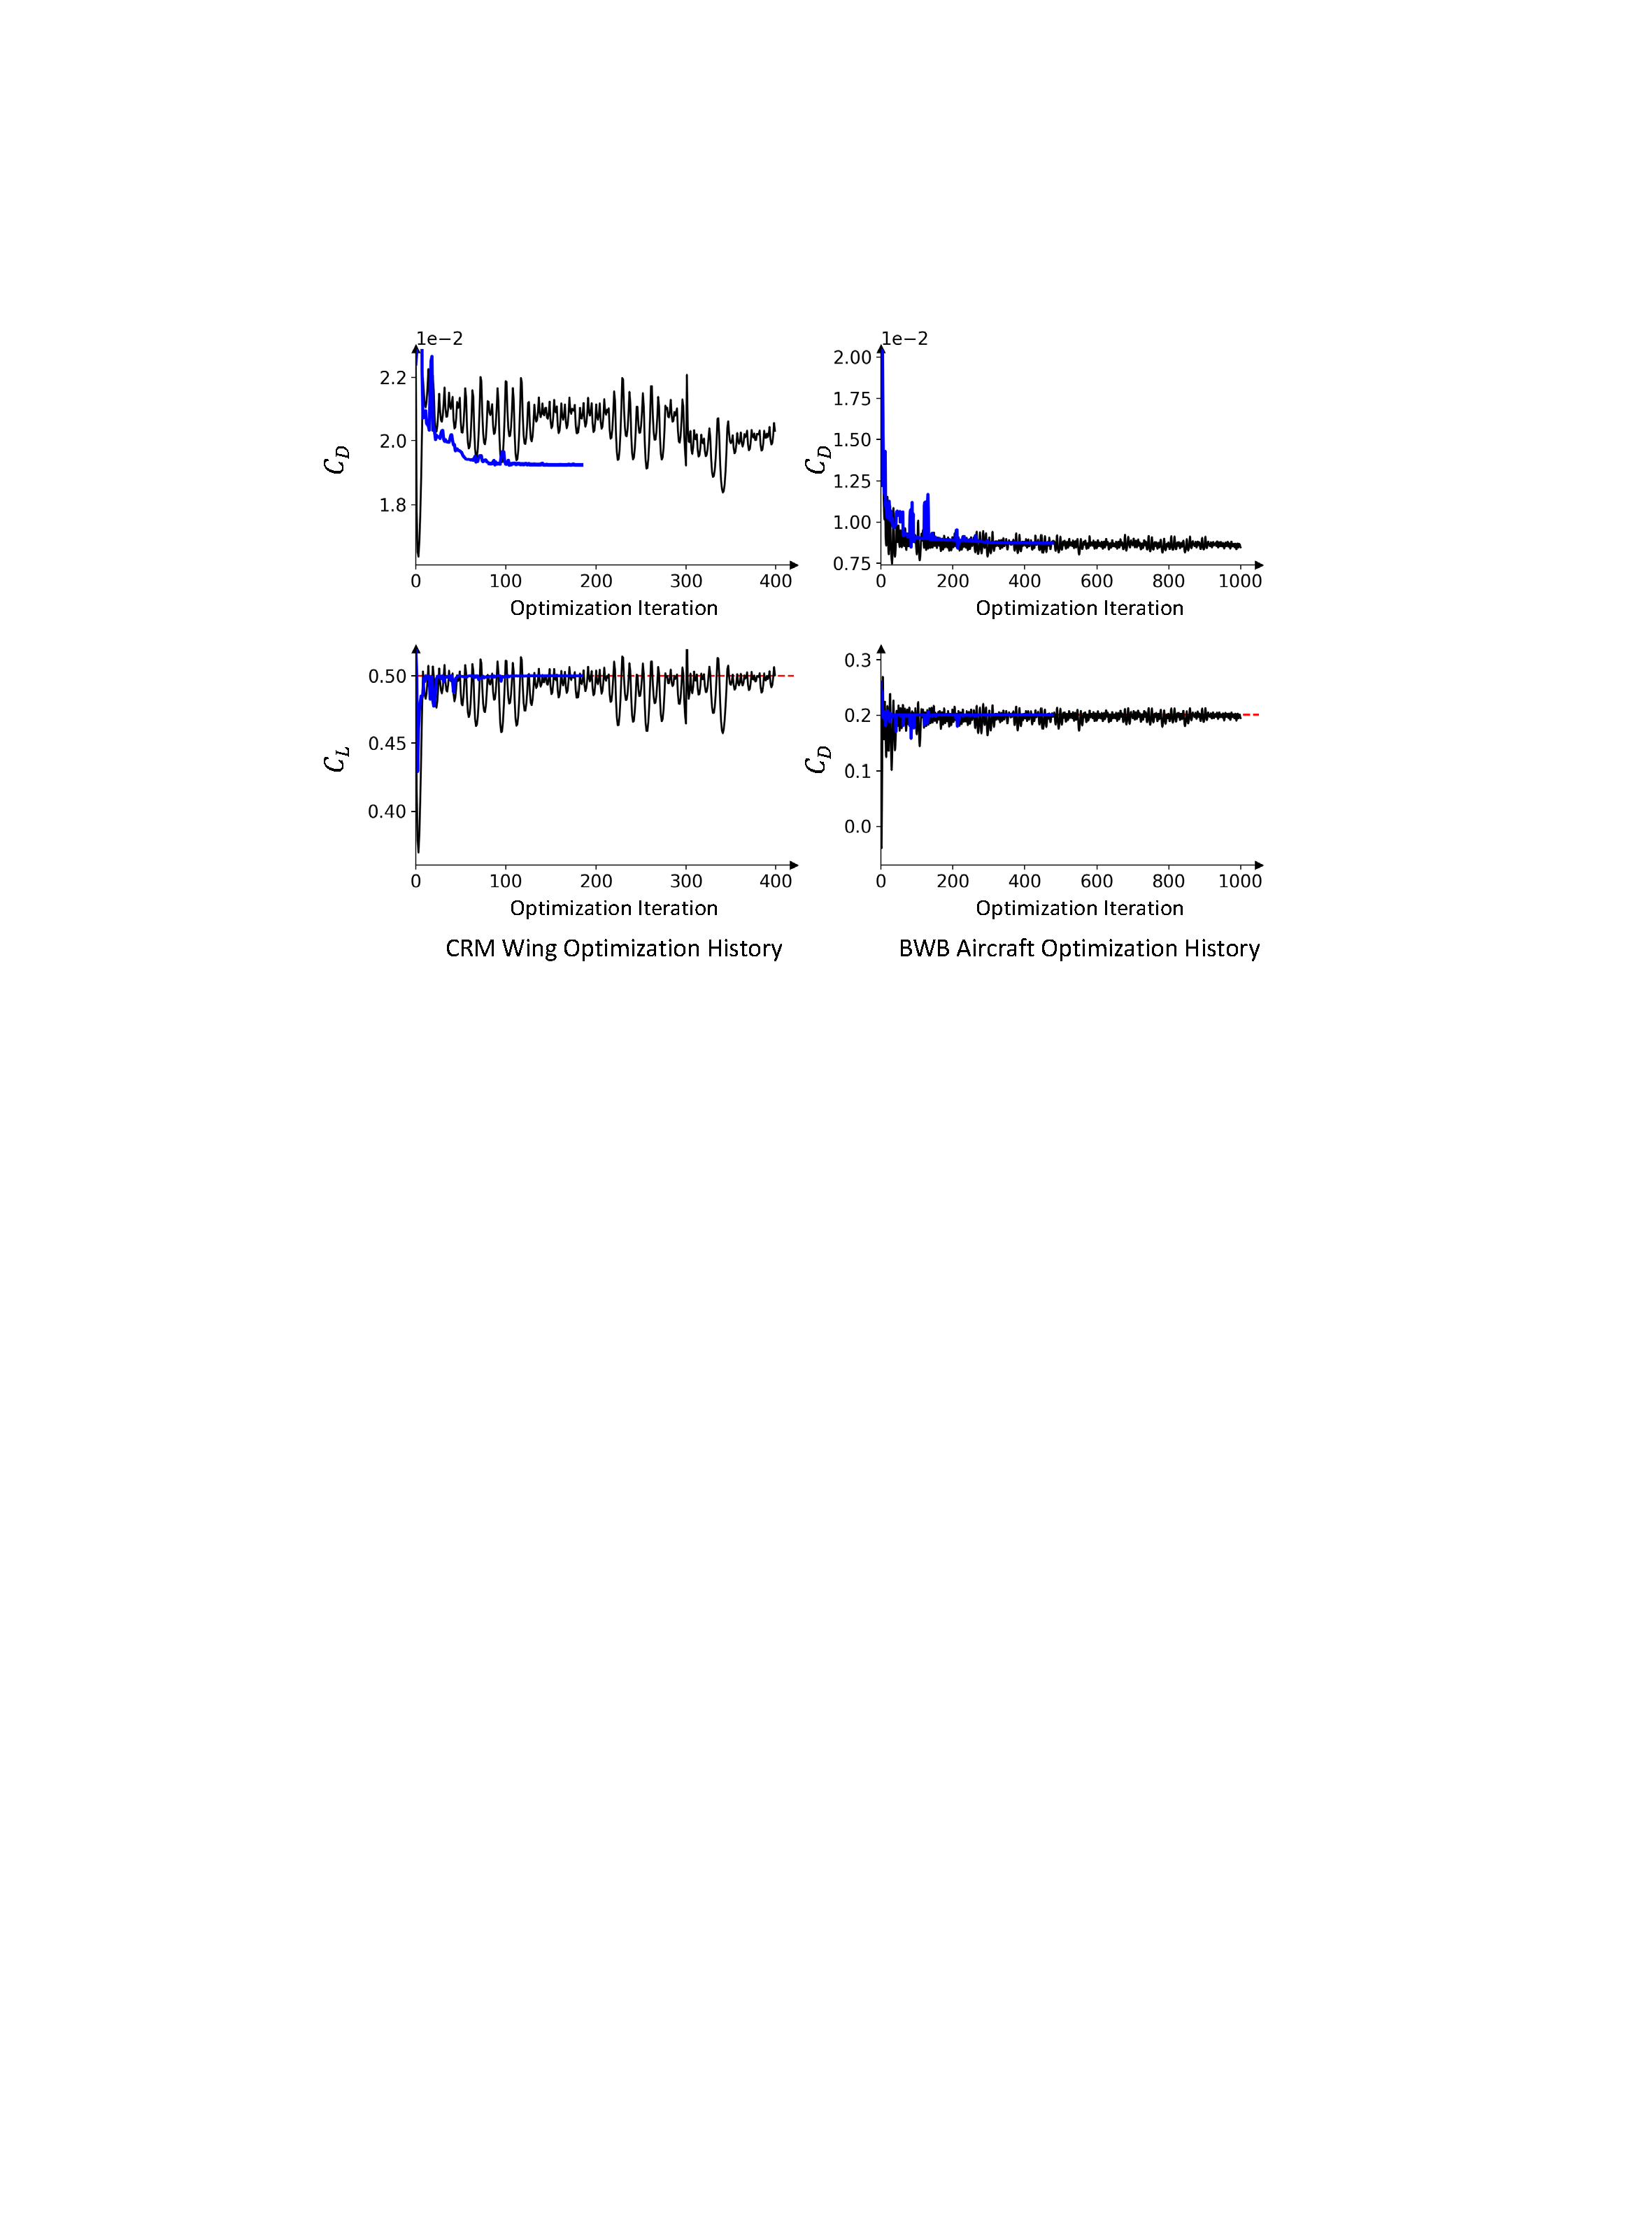
\includegraphics[width=1\linewidth]{chapter5/fig/ffd_history_comparison.pdf}
    \end{center}
    \vspace{-3mm}
    \caption{
        \small The comparison of DeepGeo-based (black) and FFD-based (blue) optimization convergence histories.
    }
    \label{ch5:fig:ffd_history_comparison}
\end{figure}

\subsection{Comparison with FFD-Based Optimization Convergence History}
\label{ch5:sec:appendix_optim_history}

Figure~\ref{ch5:fig:ffd_history_comparison} shows the convergence histories for optimizations with both FFD and DeepGeo. The CRM wing case uses 192-point FFD configuration, while the BWB aircraft case uses 240 control points. Both FFD-based optimizations use the IPOPT optimizer.

The FFD-based optimizations, as shown in blue lines, converge faster than the DeepGeo-based ones, though the number of iterations remains within the same order of magnitude. DeepGeo can achieve significant improvement at early stage, but requires more iterations to reach better optima. For example, in the BWB aircraft case, the DeepGeo-based optimization achieves a shock-free design by the 149th iteration, but continued to improve and reached higher performance after 998 iterations. DeepGeo's convergence path can be less stable due to the inefficient first-order gradient descent optimizer. We believe that further investigation into more advanced optimization strategies could improve DeepGeo's convergence behavior.